\documentclass[12pt,english]{article}
\usepackage[utf8]{inputenc}
\usepackage{tgpagella} % Palatino text only
\usepackage{mathpazo}  % Palatino math & text
\usepackage[left=1.5in,right=1.5in,top=1.5in,bottom=1.5in]{geometry}
% \linespread{2}
\usepackage[super,comma,sort]{natbib} % WPcomment
% \usepackage[round,sort&compress]{natbib} % NCCcomment
% \usepackage[natbibapa]{apacite}
% \bibliographystyle{apacite} 
\usepackage{url} % [hyphens]
\usepackage[hyperpageref]{backref} % back references biblio. Needs latexmk at compilation. Incompatible with apacite.
% \usepackage{hyperref}
\usepackage[pagebackref]{hyperref} % Incompatible with apacite.
% \usepackage{hyperref}
% \usepackage{multibib} % incompatible with backref
\hypersetup{
  colorlinks=true, % breaklinks=true,
  urlcolor=purple,    % color of external links
  linkcolor=blue,  % color of toc, list of figs etc.
  citecolor=violet,   % color of links to bibliography
}
\usepackage{bm}
\usepackage{indentfirst}
\setcitestyle{aysep={}} 
\usepackage{amsmath}
\usepackage{tcolorbox}
\usepackage{amssymb}
\usepackage{eurosym}
\usepackage{amsfonts}
\usepackage{enumerate}
\usepackage{babel}
\usepackage{graphicx}
\usepackage{caption}
\usepackage{supertabular}
\usepackage{tabularx}
\usepackage{float}
\usepackage{dsfont}
\usepackage{fancyvrb}
\usepackage{verbatim}
\usepackage{enumitem}
\usepackage{setspace}
\usepackage{comment}
\usepackage{subcaption}
\usepackage{tikz}
\usepackage{gensymb}
\usepackage{textcomp}
\usepackage{placeins} % Floats appear in their section (to use with \FloatBarrier or [section])
\usepackage{tabulary}
\usepackage{tabularx}
\usepackage{booktabs}
\usepackage{fullpage}
\usepackage{morefloats}
\usepackage{makecell}
\usepackage{lscape}
\usepackage{pdflscape}
\usepackage{longtable}
\usepackage{rotating}
\usepackage{fancyhdr}
\usepackage{tocbibind} % Adds biblio to ToC
% \usepackage{tocloft}
\usepackage{titletoc} % Adds title to ToC (use with tocloft?)
\usepackage[export]{adjustbox}
\usepackage[anythingbreaks]{breakurl} % for links
\usepackage{multicol}
\usepackage{lineno}
\usepackage{endnotes}
% \let\footnote=\endnote
% \linenumbers
\makeatletter
\renewcommand\tableofcontents{% removes "Contents" from ToC
    \@starttoc{toc}%
}
\makeatother
\newsavebox\ltmcbox % For net gain table over two columns
%\usepackage[nomarkers,figuresonly]{endfloat} % Figures at the end
%\usepackage[section,below]{placeins} % Floats placed in the section they appear in.
\renewcommand{\floatpagefraction}{.99}
\newenvironment{stretchpars}{\par\setlength{\parfillskip}{0pt}}{\par} % to justify a line

\newcommand{\gras}[1]{\textbf{#1}}
% \newcites{App}{Appendix References}

% \captionsetup[table]{skip=-10pt}
% \begin{document}

% \maketitle

% % \clearpage
% \renewcommand{\bibsection}{\section{\refname}}
% \bibliographystyle{naturemag}
% \bibliography{global_tax_attitudes}
% % \stopcontents

% \end{document}


% \title{Global Policies to Phase Out Fossil Fuels } 
\title{From Global Policies to Phase Out Fossil Fuels\\To a Sustainable Union} 

% \author{Adrien Fabre$^{1,2}$} % WPcomment
\author{Adrien Fabre\footnote{CNRS, CIRED. E-mail: adrien.fabre@cnrs.fr.}}

\date{\today} % NCCcomment

\begin{document}

\sloppy
\maketitle

\begin{center}
{\textbf{\href{https://github.com/bixiou/global_tax_attitudes/raw/main/paper/global_climate_policies.pdf}{Link to most recent version}}}
\end{center}

% WPcomment
% \begin{affiliations}
% \item CNRS
% \item CIRED
% \end{affiliations}

% \begin{small} % NCCcomment
\begin{abstract}

This paper is divided in three sections. First, I take stock of the current international climate policy regime. After showing that the current regime falls short on ensuring decarbonization aligned with the Paris Agreement's target and on providing sufficient resources for sustainable development in the Global South, I delineate the objectives that a new regime should meet. Second, I propose that voluntary countries form a \textit{Fossil-Free Union} whereby they would establish an international emissions trading system to guarantee that their emissions are in line with the target, and where the allocation of emissions rights would ensure North-to-South transfers in a way that would make most countries willing to join. Third, I propose a \textit{Sustainable Union}, where voluntary countries would commit to reallocate one percent of their GNI to all countries in proportion to their population, financed by global solidarity levies on the wealthiest. These proposals are complementary, they would put the world on track for the climate and sustainable development targets. Lastly, they garner majority support among the population in every country. 

This document will soon be expanded to include a draft treaty (translating the above proposals in legal terms) as well as a comparative analysis of alternative international climate policies.

\end{abstract}
% \textbf{JEL codes:}
% \textbf{Keywords:} 

\clearpage
\tableofcontents

% \onehalfspacing % NCCcomment

\clearpage

\section{Where do we stand? What do we need?\label{sec:now}}% NCCcomment


\subsection{A critical assessment of the current regime\label{subsec:criticism}}

The international climate policy regime is laid down in the United Nations Framework Convention on Climate Change (UNFCCC), and its offshoot, the Paris Agreement. The consensus of the international community in favor this regime and its common  temperature target is an immense success: the UNFCCC has been universally adopted, and the Paris Agreement has been ratified by all countries but three (Iran, Libya, and Yemen), before the U.S. withdrawal. As the UNFCCC takes its decisions by consensus, this also results in major limitations: agreements rest on the lowst common denominator and fall short of achieving any substantial progress on international climate action. In this section, we review the current regime and its most likely developments.

\subsubsection{Developed nations taking the lead\label{subsubsec:developed}}
The UNFCCC introduces the distinction between developed and developing nations: the former shall provide financial resources to the latter to promote their sustainable development and climate action. While aimed at sharing fairly the costs of climate action, this classification dates from 1992 and is now outdated. For example, while Singapore, South Korea, Saudi Arabia and Slovenia are all richer than Greece, only the latter is considered by the UNFCCC to be a developed country with financial obligations. This outdated classification is stalling progress in critical negotiations, as newly high-income countries resist being considered developed, and historically developed countries are reluctant to increase their contributions unless all high-income countries do so.

While high-income countries should indeed provide resources for foster climate action in lower-income countries, the determination of required transfers should not rest on an outdated, binary classification; it should be defined using up-to-date, continuous indicators such as the GNI per capita. A simple yet fair rule would be that a country's contributions are to be made in proportion to GNI and entitlements in proportion to population. 

\subsubsection{CBDR\label{subsubsec:cbdr}} 
In its Article 1, the UNFCCC states what is now known as the \textit{CBDR} principle: ``Parties should protect the climate system (...) on the basis of equity and in accordance with their common but differentiated responsibilities and respective capabilities.'' This Article is commendable in its objective to guide the allocation of the burden of climate action between countries and reconcile different burden-sharing principles: common action, equity, historical responsibility, ability to pay, etc. Unfortunately, the CBDR principle only offers vague and inconsistent guidance. For example, does equity refer to equal per capita emissions rights or to something else (equal cost of emissions reductions, equal access to development)? How should we balance rules that result in different allocations of emissions rights, such as common action, equal per capita, historical responsibilities and ability to pay? As the key question of the burden-sharing rule was left unresolved by the CBDR principle and its multiple possible interpretations, countries are not able to agree on binding targets of emissions reductions and financial transfers by country. 

\subsubsection{NDCs\label{subsubsec:ndc}} 

This absence of consensus on burden-sharing led to the system of Nationally Determined Contributions (NDCs), where each country sets its own targets. Countries are not sanctioned if they fail their targets. Countries do not even have to define their target using a common indicator (such as their future cumulative emissions). As NDCs rarely specify a cumulative emissions target, researchers need to formulate hypotheses to assess whether NDCs are jointly consistent with the universally agreed temperature target.\footnote{Note that the temperature is itself vague. Article 2 of the Paris Agreement aims at ``holding the increase in the global average temperature to well below 2~\textdegree{}C above pre-industrial levels and pursuing efforts to limit the temperature increase to 1.5~\textdegree{}C above pre-industrial levels.'' Yet, given the uncertainty around the climate system, this (double) target is not precisely defined: does it mean a 83\% chance to limit global warming to 2~\textdegree{}C? A 67\% chance? A 50\% chance? Each probability is associated with a different carbon budget -- respectively 900, 1,150, and 1,350 GtCO$_\text{2}$ starting in 2020, according to the IPCC (AR6, WGI, p. 39).} 
Even in the most optimistic hypotheses, NDCs are insufficient to meet the temperature target. If all countries respect their NDCs, global GHG emissions should be 51~GtCO$_\text{2}$e in 2030, while 41~Gt would be needed to meet the 2~\textdegree{}C target with a 66\% chance.\cite{den_elzen_updated_2022} According to the \href{https://climateactiontracker.org/}{Climate Action Tracker}, 
current policies and actions correspond to a global warming of +2.7~\textdegree{}C by 2100, a warming may continue to rise beyond that date.

\subsubsection{ITMOs\label{subsubsec:itmo}} 

The article 6.2 of the Paris Agreement allows Parties to exchange Internationally Transferred Mitigation Outcomes (ITMOs). This enables a country to nominally reduce its emissions (the emissions as counted to assess its NDC) by purchasing an ITMO to another country. The latter country will then be credited with the buyer's ITMO emissions. As any bilateral agreement on ITMO is permitted, the use of ITMOs risks reducing the buyers' domestic decarbonization efforts. % Take Switzerland's purchase of ITMOs from Thailand: if they meet their target, these two countries will jointly reach 5.5~tCO$_\text{2}$e per capita in 2030, more than the global level of 4.5~tCO$_\text{2}$e that would be in line with the 2\textdegree{}C target. This observation alone is insufficient to state that these two countries lack climate ambition: for example, if Switzerland and Thailand had the same NDCs but other countries had more ambitious ones, such that the world total is in line with the temperature target, 
Indeed, to the extent that the NDCs do not add up to the global emissions reductions objective, ITMOs would not reflect the required mitigation constraint, and their price of ITMOs will be too low. As a result, ITMOs may propagate a global lack of ambition to countries with otherwise ambitious NDCs, offering a cheap (and less effective) alternative to domestic decarbonization. 
% To the extent that the sum of NDCs' mitigation efforts falls short of the global target, the price of ITMOs will be too low. 
% In other words, the lack of ambition of some countries' NDCs can propagate to other countries through the sale of ITMOs. 
% mention "hot air"?

To prevent ITMOs from weakening domestic action, countries that use them should commit to extra rules, beyond verifying the environmental integrity of the ITMO they buy. In case of linkages between domestic carbon markets, the same rules would be required to the cross-border (or rather, cross-market) purchase of emissions allowances. Let us call \textit{sellers} the countries that are willing to sell ITMOs, and \textit{buyers} the countries they agree to sell them to. The extra rules could be as follows: 
\begin{itemize}
  \item Sellers and buyers should include a cumulative emissions target (i.e. a national carbon budget) in their NDC, decomposed in yearly targets.
  \item The joint carbon budget of sellers and buyers should be compatible with the Paris temperature target. If the group sellers and buyers does not include all countries, their joint carbon budget should correspond to their population share of the world's budget.
  \item The joint carbon budget (of sellers and buyers) in a given year should be lower than their preceding year's joint emissions, by at least (say) 2\%.
\end{itemize}

If a group of sellers and buyers agrees to these rules, they would effectively impose the principle of an equal per capita allocation of emissions rights, at least to govern the allocation between their group and the rest of the world. While alternative allocation principles are possible, the operationalization of the cross-border trading of emissions allowances (or ITMOs) needs to rely on an allocation principle. The inadequacy of NDCs (taken jointly) proves that the global climate regime cannot rely on diverse and self-serving allocation rules to divide the global carbon budget into consistent national targets. 


\subsubsection{Climate finance\label{subsubsec:finance}}

An equal per capita allocation of emissions rights corresponding to the remaining carbon budget would entail transfers approaching 1\% of the world's GDP (or \$1 trillion per year) from high to low emitters, that is from the Global North to the Global South. Taking into account historical responsibilities for emissions, an equal per capita allocation of cumulative (past and future) emissions rights would entail even more transfers (the carbon debt that the North owes to the South is estimated at \$26 trillion\cite{fabre_global_2024}). 

At COP29, the international community reached a compromise concerning the New Collective Quantified Goal (NCQG): Developed countries committed to mobilize \$300 billion per year by 2035 for developing countries for climate action (and countries ``call on all actors'' to mobilize \$1.3 trillion, which would be in line with experts' recommendations\cite{unfccc_new_2024,songwe_raising_2024}). Although the quantum of \$300 billion represents a tripling of the previous climate finance goal, it can be reached through loans (including from the private sector), and does not specify what share should be provided as grants (or grant-equivalent concessional loans). In fact, the current goal of \$100 billion is met with only \$26 billion provided in the form of grants. In theory, the NCQG could be met with the same amount of grants (i.e. North-to-South transfers), or even less. 

In contrast, at COP29, ``India specified that the NCQG should mobilize \$1.3 trillion, of which at least \$600 billion should come in the form of grants and equivalent resources.''\cite{earth_negotiations_bulletin_daily_2024} India, voicing Global South concerns, stated it was ``disappointed in the outcome which clearly brings out the unwillingness of the developed country parties to fulfill their responsibilities. We cannot accept it.'' Transfers aligned with Global South's demands would allow enormous progress towards the Sustainable Development Goals, including climate action but also the deployment of public services and poverty reduction programs. Conversely, an insufficient provision of climate finance does not only infringe on climate justice, it also jeopardizes decarbonization in the Global South, as many countries make their NDC conditional on the adequate provision of climate finance. 

Together with more North-to-South transfers, reforms to the international financial systems are needed to reorient financial resources towards climate action. These reforms are multifaceted and are more likely to be accepted by governments in the Global North than direct transfers, since that they rely on mostly painless, growth-enhancing accounting operations. The government of Barbados (supported by the UN Secretary-General) leads the movement in favor of these reforms. Their ``Bridgetown Initiative'' calls for debt relief for low-income countries, for a new issuance of at least \$650 billion in Special Drawing Rights by the IMF to expand the loans of Multilateral Development Banks (MDBs) to at least \$500 billion per year, and for public guarantees to lower interest rates on sustainable projects in the Global South.\cite{bridgetown_bridgetown_2025} Note that although the Bridgetown Initiative is most famous for its climate finance proposals, it also calls for other reforms, such as a universal carbon price and international taxes on the super-rich funding global public goods. 

While a scaling up of climate finance is crucial, it is not sufficient to decarbonize the world as it does not cap (or directly reduce) emissions. In the worst case scenario, the expansion of low-emissions projects would mostly add up low-carbon infrastructures on top of fossil ones, failing to meaningfully reduce emissions.

\subsubsection{JETPs\label{subsubsec:jetp}}

The last piece of the climate regime worth mentioning is the Just Energy Transition Partnerships (JETPs). JETPs are mechanisms where one developing country essentially commits to emissions reductions through the deployment of renewable energy in exchange for concessional terms on the required loans by a group of developed countries. Four JETPs have been signed so far, involving Indonesia, Vietnam, South Africa, and Senegal.\cite{ha-duong_just_2023} In existing JETPs, the groups of developed countries pledged to offer loans ranging from \$2.5 billion (for Senegal) to \$20 billion (for Indonesia). 

While JETPs offer a promising way to deliver climate finance in a way that guarantees emissions reductions, they currently suffer from several shortcomings. First, their coverage is limited (in terms of sectors and countries). To improve the sectoral coverage and efficiency of JETPs, researchers have proposed to design them as a financial transfer in exchange for a national carbon price. Second, as they focus on emissions reductions rather than sustainable development, JETPs do not contribute to poverty reduction. This concern could be mitigated by JETPs with a higher reliance on grants.\cite{bolton_why_2025} However, a higher provision of grants is difficult to achieve absent a dedicated source of revenue (such as an international tax).
% cite those who say they should be grant based and those who say they should involve pricing/regulations

Lastly, even if JETPs were improved along the previous lines, they would still fail to guarantee that the decarbonization of big emitters like China or the European Union is consistent with required global efforts. 

% I. current model: NDCs (pb: don't sum up to carbon budget, no common burden-sharing norm), ITMO (pb: hot hair), JETPs (pb: limited coverage, even if expanded wouldn't guarantee big emitters like China or EU decarbonize, absence of funding mechanism, don't address poverty); Bridgetown (necessary but insufficient as doesn't cap emissions)

\subsection{Objectives for a truly sustainable regime\label{subsec:objectives}}

Now that we have a critical understanding of the current international climate regime, let us sketch the properties we desire for a new (or improved) regime. We will then be able to assess different proposals in light of these objectives. Here they are:
\begin{itemize}
  \item \textbf{Temperature}. An effective climate regime should achieve the Paris Agreement's temperature target. It should do so by a stabilization of the concentration of each GHG in the atmosphere, and abstain from climate engineering risky bets such as Solar Radiation Managements. This objective would translate into a global carbon budget. For example, the carbon budget could be set at 1,000~GtCO$_\text{2}$ starting in 2025, which corresponds to most likely warming of +1.8\textdegree{}C a 67\% chance to keep global warming below +2\textdegree{}C. 
  \item \textbf{SDGs}. A holistic approach requires solving all humanity's greatest challenges, not just climate change. As explained above, climate justice requires sufficient North-to-South transfers to fund sustainable development (not just climate action). Even though the Sustainable Development Goals (SDGs) and the planetary boundaries would require additional policies and transfers, one important feature of the climate regime is how much climate finance it delivers in the form of transfers to the poorest and improved market conditions. This can be measured through SDGs indicators or GDP per capita in low- and lower-middle-income countries.
  \item \textbf{Efficiency}. As stated by the UNFCCC since 1992,\cite{unfccc_united_1992-1} ``measures to deal with climate change should be cost-effective so as to ensure global benefits at the lowest possible cost.'' Economists have shown that ensuring cost-effectiveness require an economy-wide carbon price, uniform across sectors and countries. This fundamentally results from the fact the social cost of emissions are independent from their source or location, therefore they should be priced uniformly. %Efficiency can then be measured by the dispersion of (implicit) carbon prices across countries and sectors. 
  Note that this argument in favor of carbon pricing does not preclude other, complementary policies: these have also been shown to be optimal by economic analysis.\cite{stiglitz_addressing_2019}
  \item \textbf{Acceptability}. An interesting international agreement is one that has good chances to be accepted by most countries. To measure the success of a proposal, we can use the share of global emissions that are covered by participating jurisdictions. Different elements contribute to acceptability: 
  \begin{itemize}
    \item \textit{Progressivity at the top}. If costs are concentrated on the richest households, the regime can benefit the majority in each country while addressing the excessive level of inequality.
    \item \textit{No loss in middle-income countries}. Countries whose population is not rich should not lose from an international climate policy. To assess whether a country loses or not, we should compare its situation in the new regime compared to the status quo. If we synthesize a country's situation by the carbon budget it is granted, a country would lose if its carbon budget is lower than their unconditional NDC completed by the ambitious emissions trajectory that the country currently envisions. % TODO? add? This challenges the blunt application of the equal per capita allocation of emissions rights, as it would entail transfers from countries with a carbon footprint greater than the world average to countries with a footprint lower than the average. Yet, some middle-income countries such as China, Iran, or South Africa, have a carbon footprint greater than the world average. 
    \item \textit{Win-win}. While (per the SDG objective) transfers would be required from high-income countries, this does not necessarily mean that these countries' population would lose out. First, because (as stated above), redistributive policies can concentrate the costs on the richest households in their country. Second, everyone would benefit from a stabilized climate and from a world where SDGs are met. For example, sustainable development would spur global demand, including for advanced technology and low-carbon exports from industrialized economies. Third, while transfers imply a loss compared to the situation with the same worldwide decarbonization efforts and without international transfers, the latter situation is unlikely (as transfers are necessary to promote decarbonization in the Global South). As above, the situation that should be used as a point of comparison is the status quo where the country's carbon budget corresponds to its unilaterally planned emissions trajectory and where there is no international trade in emissions allowances. To the extent that transfers are the counterpart of the purchase of emissions allowances, a new climate regime could be a \textit{win-win} for all participating countries, as they would all reap the efficiency gains of an optimal location of emissions reductions.
  \end{itemize}
\end{itemize}
% objectives: SDGs (=> transfers / climate finance), 2°C, efficiency (say it's in UNFCCC 92, => uniform price), acceptability (=> concentrate costs on richest, coalition of willing, win win thx to efficiency, LMIC not losing (compared to carbon budget corresponding to their unconditional ambitious scenario)), incentives to expand (remove?)

\paragraph{Coalition of the willing}. International negotiations have shown that it is illusory to seek universal agreement for an ambitious agreement. Therefore, political realism requires pushing for proposal that do not get accepted by all countries, and thus, that may also fail to deliver on the climate target, as countries outside the coalition would not fulfill their part of the temperature objective. If oil exporting countries, representing 25\% of current emissions, do not join the coalition, temperature in 2100 would be about 0.3\textdegree{}C higher than with a universal participation to decarbonization efforts. While this outcome would be a partial renouncement to some objectives (full acceptability, temperature target), it is probably the only type of outcomes that is accessible given the political balance of power.

% \clearpage
\section{A Fossil-Free Union\label{sec:ffu}}

Having in mind the shortcomings of the current regime as well as the objectives of a new regime, we are now equipped to propose an international agreement to phase out fossil fuels in way that is cost-effective, promotes sustainable development, and acceptable to most countries. % TODO! elite support: Rajan, vdL, Dasgupta, Blanchard-Tirole...

\subsection{The principles for a Fossil-Free Union\label{subsec:principles}}

The Union would be open to any country, as well as subnational entities (such as U.S. states). 

\paragraph{Emissions Trading System}
The Union would put in place an international Emissions Trading System (ETS), that would add up to existing ones (to not dilute the stringency of existing ETSs). All sectors except agriculture and land-use (LULUCF) would be covered. In particular, the ETS would cover (domestic and international) aviation. International shipping could also be covered, replacing the system established by the International Maritime Organisation. The ETS would cover all gases emitted in industrial or energy processes, as in the Korean ETS. Namely, the ETS would cover CO$_\text{2}$, N$_\text{2}$O, PFCs, SF$_\text{6}$, HFCs, as well as methane emissions from industrial processes, fossil fuel extraction, and waste management (but not methane emissions from agriculture). %As in existing ETSs, production units below a minimal threshold would be exempted. % TODO which equivalence between GHG

Complementary policies such as the Tropical Forest Forever Fund would be needed to cover LULUCF sectors. This is important to avoid carbon leakage that would substitute fossil fuels by biomass obtained through deforestation.

Emissions allowances would be fully auctioned by an ad hoc international authority to polluting companies upstream of the supply chain. 

The ETS will be completed by a carbon border adjustment to prevent carbon leakage and ensure that the Union's carbon footprint (rather than its territorial emissions) is capped. Importers into the Union would have to purchase emissions allowances corresponding to the carbon embedded in the imported goods. Exporters out of the Union would receive a rebate for the carbon embedded in their exports, and extra allowances would be auctioned to finance the rebates. 

In some federal countries like the U.S., some States may be willing to join the GCP while the federal level would not. To help such States to join the Union despite their belonging to a national customs union, they would be exempted from the carbon border adjustment. In this way, a State like California could join. It could also use its share of the revenues to subsidize manufacturing firms, perpetuating its way of recycling ETS revenues and preventing carbon leakage.

Once export rebates are paid, the remainder of carbon pricing revenues would be returned to countries based on their yearly carbon budget.


\paragraph{National carbon budgets}
Each country would be granted a carbon budget between the starting year (say 2030) and net-zero (say in 2080). 

Each country would then describe how they would divide their carbon budget intertemporally. As such, the yearly trajectory of the Union's emissions over the next fifty years would be known at the starting year. Each country would be relatively free on the intertemporal breakdown of their carbon budget, though this choice would have to respect some constraints, developed in Section \ref{subsec:implementation}, and related to the rules to avoid hot hair proposed in Section \ref{subsubsec:itmo}.

\paragraph{Adjusted per capita allocation}
By default, each country would be granted a carbon budget corresponding to an equal per capita share of the remaining global carbon budget. This allocation can be understood as an equal right to pollute for each human, irrespective of their country. Such an allocation would induce international transfers from agents (people or countries) with a carbon footprint higher than the world average, to agents with a lower carbon footprint.

As future population is unknown (and can be affected by policy choices), the benchmark per capita carbon budget would be based on the population share taken at the starting year. % Also, compared to children, adults are predominantly responsible for GHG emissions and most adults over the 2030--2050 period (the most crucial for emissions reductions) will be born in 2030.
Then, some departures from the benchmark would allow adjusting to special circumstances.

To prevent transfers flowing from lower-income countries to high-income countries, high-income countries would be granted a carbon budget corresponding to their ambitious decarbonization pathway. In particular, the European Union would be granted emissions allowances in line with its NDC, with 90\% emissions reductions in 2040 (compared to 1990), and net-zero in 2050. This represents less than half of EU's benchmark equal per capita share.

To prevent middle-income countries from being net contributors of international transfers, countries would be allowed to propose further departures from the benchmark allocation, to the extent that the Union's carbon budget is respected. These departures from the benchmark need to be agreed by a majority of participating countries, weighted by their GHG emissions. % TODO! refine

In particular, middle-income countries with emissions per capita above the world average, such as China, Iran, or South Africa, could be granted a carbon budget equal to the cumulative carbon footprint corresponding to their own ambitious decarbonization pathway.

\paragraph{Universal cash transfer} 
The Union would encourage countries to return the ETS revenue to the population through an equal cash transfer. In particular, the Union would develop standard and provide technological resources to distribute the cash transfer. Despite the difficulty to reach people who lack civil status or live in remote areas, solutions exist. For example, the Indian system Aadhaar provided a unique biometric identifier to 99\% of the country's population in less than seven years. In Africa, the World Bank's ID for Development program is financing the deployment of universal legal identity, in line with SDG Target 16.9. Besides, with phone-based payments and biometric identification, satellite Internet, and off-grid solar panels, the technology is mature and affordable to distribute cash transfers in a way that is fraud-resistant and leaves no one behind.

The equal cash transfer would compensate people for the rise in fossil fuel prices. The transfer would reflect each person's equal right to pollute, as it would work as if the person would have sold this right to polluting companies at the carbon price.

Countries that choose not to distribute all revenue through a cash transfer would have to prove that they spend it %on social protection, public services, and infrastructure, 
in a way that leaves no one behind.

% Second, the basic income must be accessible to all and fraud-resistant (so that no one receives the basic income twice). It is difficult to reach people who do not have a civil status or who live in remote areas. Likewise, it is difficult to verify people's identity and to be confident that they are not registered multiple times. However, there are good reasons to be confident that the required infrastructure to deliver a basic income can be deployed within ten years, as different technical solutions are available. First, most countries maintain electoral lists and already have social programs targeted to isolated people. Second, smartphones now provide biometric identification as well as a costless means of transaction (and the cost of a smartphone would be covered by just a few months of basic income). Third, while many places are still lacking internet access, progress is rapid in satellite internet access, and it might soon become cheap and ubiquitous \citep{hanson_satellite_2016}. Fourth, experience can be gained from the Aadhaar system, launched in 2009, which now provides to 99\% of the Indian adult population a unique biometric identifier. Aadhaar is linked to one's bank accounts and used to distribute welfare benefits. Although the technical challenge remains, it seems solvable by an appropriate combination of these solutions, tailored to the specific needs of each region. 

\subsection{Likely participating countries\label{subsec:scenarios}}

Countries that would not lose from the policy are expected to join: these include all low- and middle-income countries, as well as high-income countries with an ambitious decarbonization plan. The map in Figure \ref{fig:participation} shows which countries are likely to join the Union. These countries represent 74\% of current emissions. % (club_emissions_share <- sum(df$emissions_2025[setdiff(df$code %in% c(union_high, "TUR", "CHL", "URY", "TUN", "UGA", "SDN", "MYS", "UKR", "TKM"), "CAN")])/sum(df$emissions_2025)) # 74%

\begin{figure}[h]
  \centering \caption{Countries likely to participate in the Fossil-Free Union.}\label{fig:participation}
  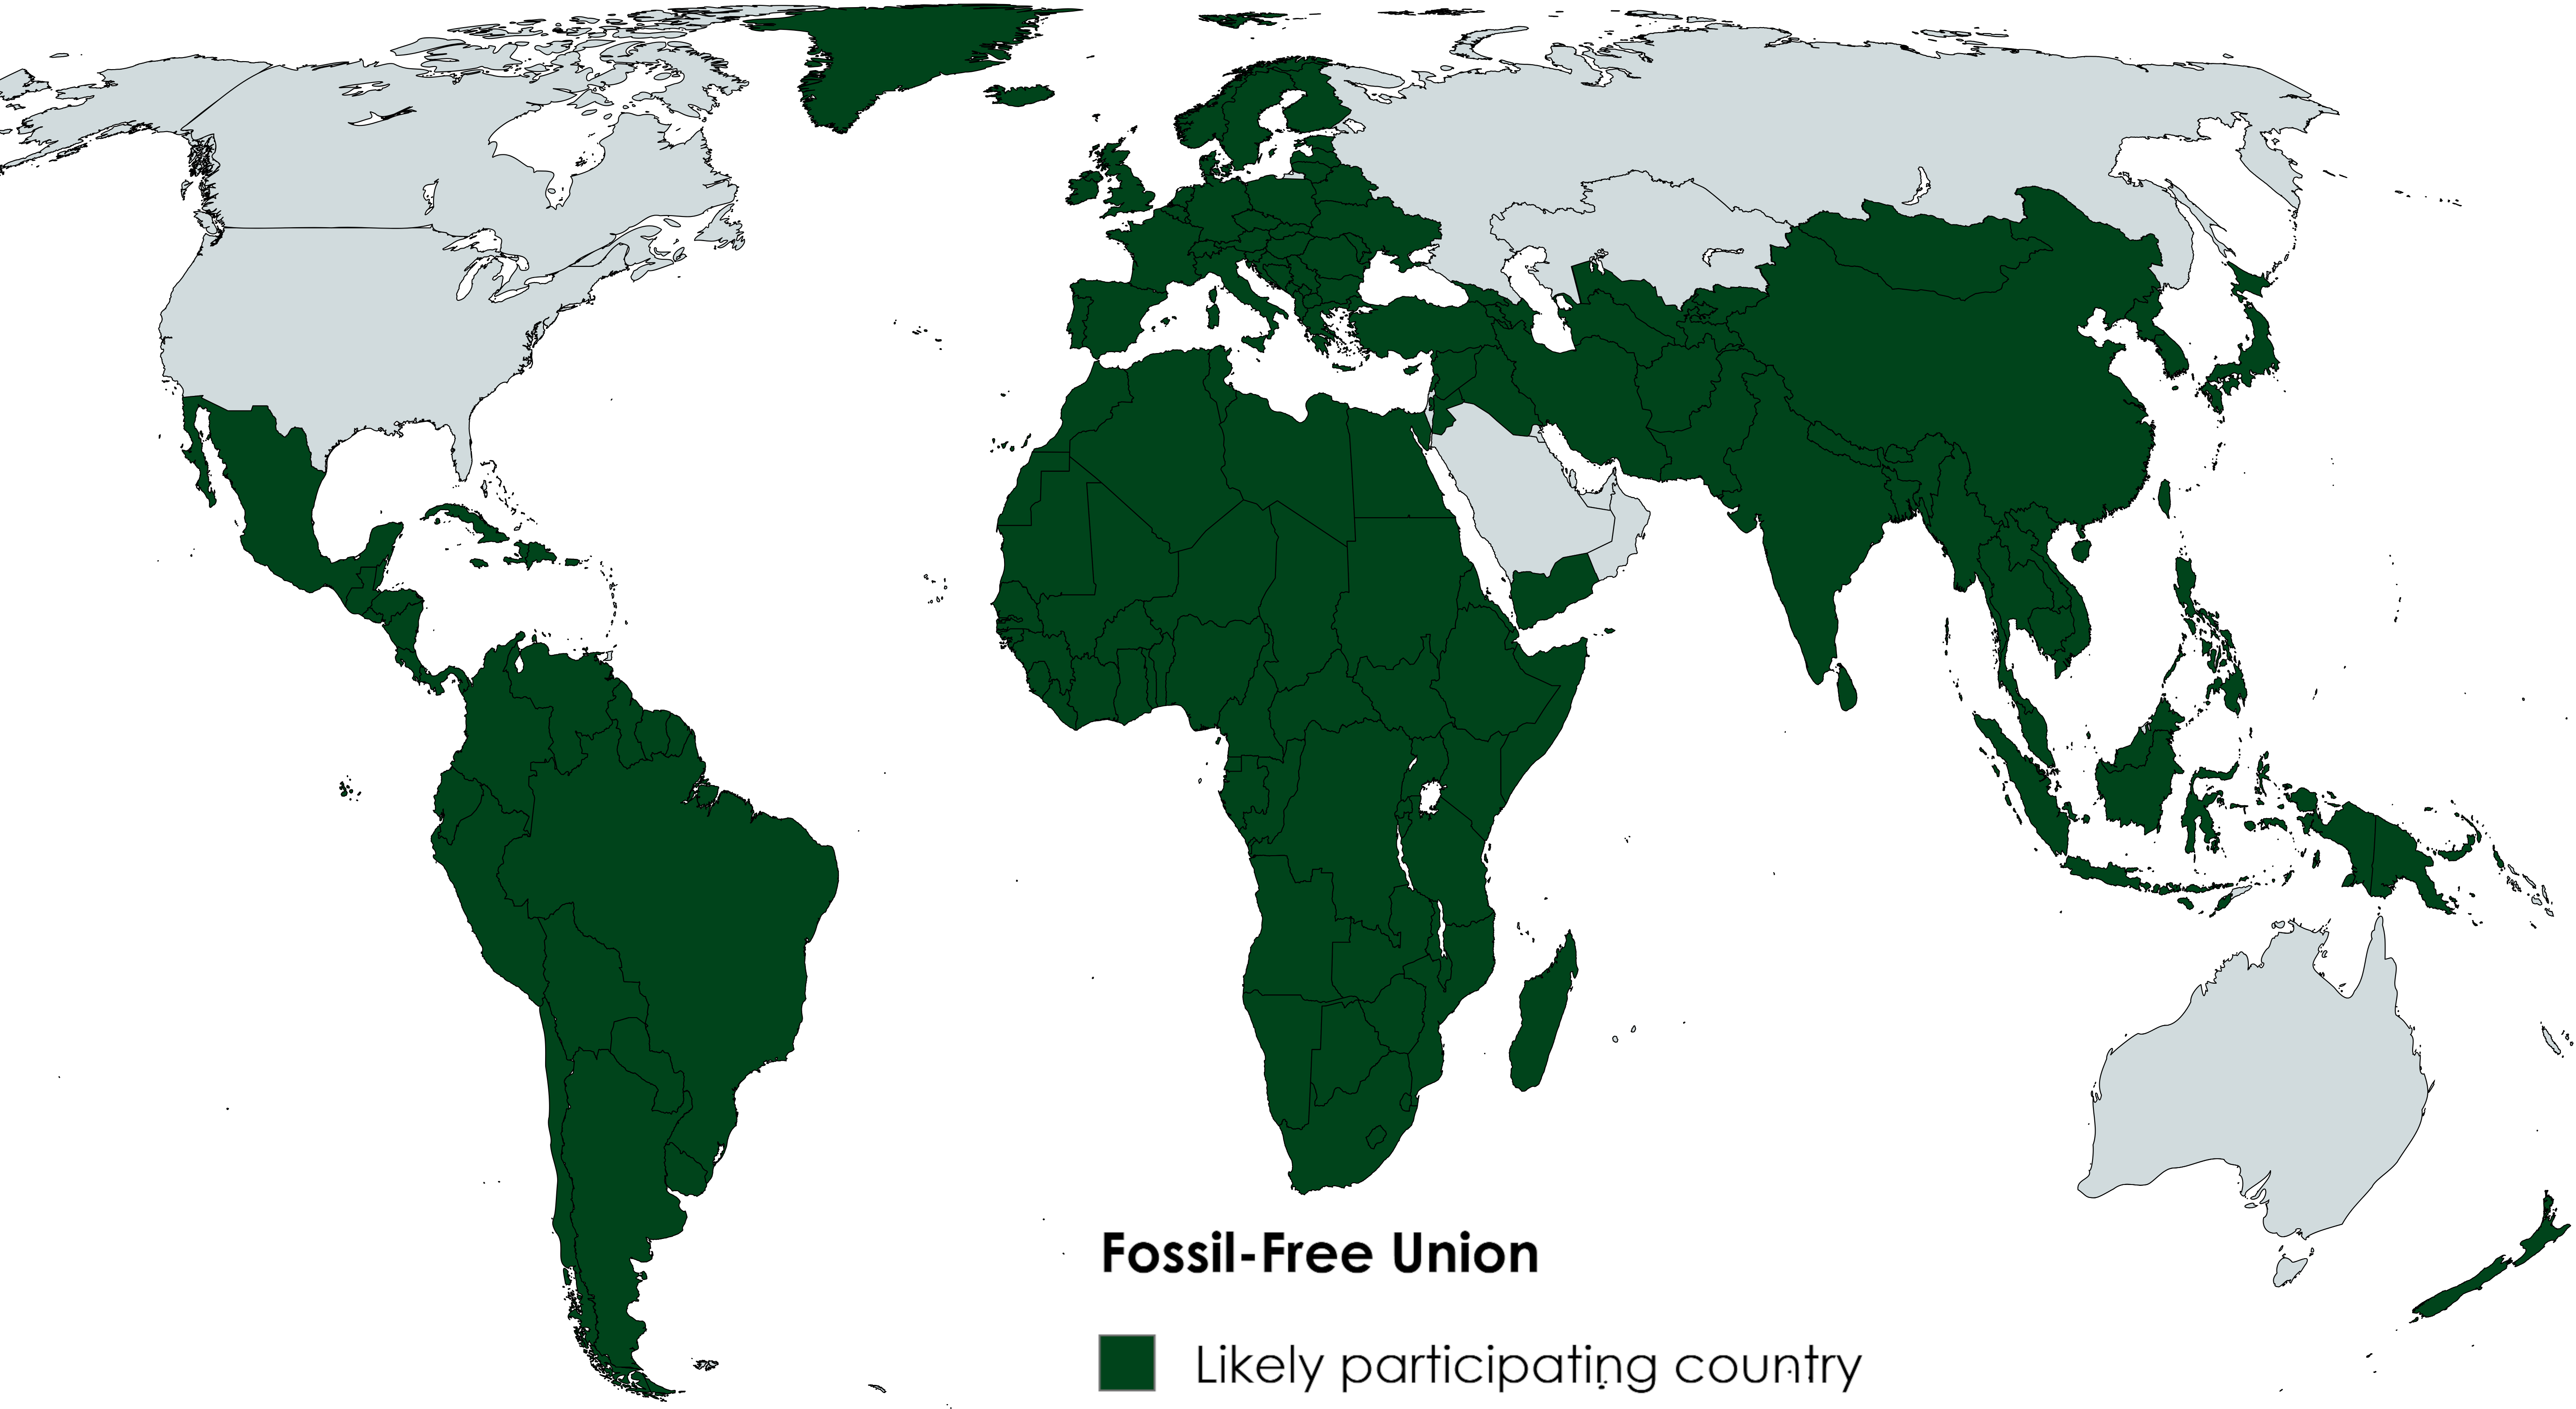
\includegraphics[width=\textwidth]{../figures/maps/participation_FFU_wo_CAN.png} 
\end{figure}
% /!\ Turkey, Iraq, Iran, and some other MEA countries are not counted in the Union in the code

\subsection{Allocation of emissions rights\label{subsec:allocation}}

Policies currently implemented in the prospective Union would imply emissions of 792~GtCO$_\text{2}$ over 2030--2080, while current NDCs (without accounting for long-term targets) would imply 708~GtCO$_\text{2}$. In both cases, emissions are expected to continue after that date.\footnote{The data on emissions by region from current policies and NDCs (with and without long-term targets) is given by van de Ven et al. (2023)\cite{van_de_ven_multimodel_2023}. Post-2030 action is modelled by extending the average rate of change in emissions intensity of GDP from 2020 to 2030. The global carbon budget (and associated equal per capita rights) follows the scenario SSP226MESGB of Gütschow et al. (2021).\cite{gutschow_country-resolved_2021}} % Post-2030 action is then modelled by measuring the average rate of change in emissions intensity of GDP from 2020 to 2030 in each region and assuming emissions-intensity reduction rates will remain the same after 2030. 
In contrast, enforcing an equal per capita share of the remaining carbon budget would limit Union's emissions to 653~GtCO$_\text{2}$ over the period and would achieve net-zero emissions by 2080.

To determine the ``non-losing'' carbon budget, below which a country could be considered losing, we proceed as follows. For countries with emissions per capita lower than the world average, we use a Contraction \& Convergence benchmark, whre emissions rights per capita start at their value in 2030 for current policies and linearly converge to the equal per capita share in 2050. This benchmark implicitly assumes that countries with relatively low emissions would consider as beneficial to their development the pathway that starts with current policies, gradually grants them extra resources for sustainable development (by rights converging to an equal per capita share of the global sum), and then make them to follow the world decarbonization trend. 
For high-income countries and for China, we use the cumulative emissions implied by their NDCs and long-term targets.\footnote{For China, the value is in line with the domestic 2\textdegree{}C target scenario developed at Tsinghua University.\cite{he_towards_2022}} Doing so implicitly assume that these countries have the domestic capacity to deliver their long-term targets on their own. These carbon budgets imply slightly more rights than the equal per capita share for China, and less for high-income countries. 

Table \ref{tab:budgets} present the cumulative emissions implied by current policies, \textit{non-losing} budgets, equal per capita ones, and the proposed allocation. The proposed allocation departs from the equal per capita one for China and Western Europe only, which are both allocated a carbon budget corresponding to their NDCs and long-term targets. It is worth noting that the proposed allocation grants Eastern Europe, Japan, and South Korea with their equal per capita share. Indeed, these countries are less rich or have significantly higher emissions per capita than the world average (contrary to Western Europe). Therefore, there is few concern that these countries would turn net recipient from international transfers and no need to apply to them the same exception as for Western Europe. % In addition, granting these countries with their equal per capita share improves acceptability. 

\begin{table}[h]
  \caption{Carbon budgets over 2030--2080 for a 1.8\textdegree{}C trajectory (in GtCO$_\text{2}$).\label{tab:budgets}} 
  \makebox[\textwidth][c]{
\begin{tabular}[t]{cccccccccc}
  \toprule
   & Africa & China & \makecell{Latin\\America} & India & Europe & \makecell{Japan \& \\South Korea} & \makecell{Other\\Asia} & \makecell{\textit{Fossil-Free}\\\textit{Union}} & \textit{World} \\
  \midrule % TODO? Add BAU?
  \textbf{Current policies} & 88 & 226 & 80 & 143 & 31 & 46 & 179 & \textit{792} & \textit{1,214} \\
  \textbf{Non-losing} & 124 & 147 & 57 & 115 & 22 & 11 & 104 & \textit{589} & \textit{786} \\ % emissions_cc for all but WEU, JPN, SKO, CHI: emissions_ndc, and world as a whole: emissions_cc
  \textbf{Equal p.c.} & 144 & \textbf{134} & 62 & 135 & \textbf{49} & 16 & 113 & \textit{653} & \textit{754} \\
  \textbf{Proposal} & 144 & \textbf{147} & 62 & 135 & \textbf{23} & 16 & 113 & \textit{640} & \textit{754} \\        
  \bottomrule\\[-0.81em]
\end{tabular}}
\end{table}% TODO! adjust China's budget to account for carbon footprint
% TODO! Correct to take out negative values (which erroneously lower the carbon budget)

Table \ref{tab:budgets} shows that the sum of the Union's proposed carbon budget is 13~GtCO$_\text{2}$ (or 2\%) lower than its equal per capita share of the world's carbon budget. The unallocated emissions allowances could be used to grant additional countries some extra carbon budget. For the moment, we have only modelled such a departure for China, but a similar one should be granted to other fossil-dependent middle-income countries with relatively high emissions: Algeria, Kazakhstan, Iraq, Iran, Libya, Mongolia, South Africa, and/or Turkmenistan. These countries currently represent 5.6\% of global emissions and 3.4\% of global population, translating into an equal per capita carbon budget of 22~GtCO$_\text{2}$; so the extra allowances would cover their needs. 

% \begin{figure} 
%   \centering \caption{CO$_\text{2}$ emissions allowances for selected regions (in tCO$_\text{2}$ p.c.).}
%   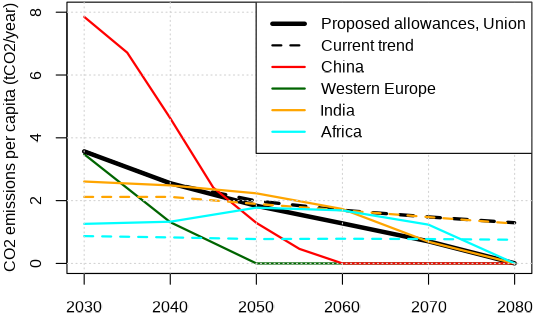
\includegraphics[height=.6\textheight]{../figures/policies/fossil_free_union_emission_trajectories.png} % TODO! remove South America from legend, have Africa converge to 0, avoid allowances > current policies
% \end{figure}

% TODO! proposed trajectories

\subsection{A win-win deal\label{subsec:winwin}}

Each country colored in Figure \ref{fig:participation} would have an interest to join the Union: 
\begin{itemize}
  \item Every country would benefit from a stabilized climate, and from the guarantee that all countries in the Union decarbonize.
  \item Most countries (including all countries likely to join) would be granted a carbon budget sufficient to avoid a loss from the status quo. Exceptions include Russia, Saudi Arabia and other high-income countries from the Gulf with low climate ambition. Even the U.S., Australia and Canada would enjoy a non-losing carbon budget.
  \item Lower-income countries would receive transfers from the rest of the world, spurring their sustainable development.
  \item Countries with an important low-carbon industry, such as East Asian countries, would gain from the stronger demand for these goods.
  \item High-income countries would benefit from the efficiency gains allowed by international carbon trading.
  \item Large representative surveys show strong public support in favor of the Fossil-Free Union, even in high-income countries when transfers are presented as a loss and the amount of transfers is specified. For example, there is 54\% support in the U.S. and 76\% in Western Europe.\cite{fabre_international_2023} % TODO update citation
  Moreover, academic research shows that political programs containing the Fossil-Free Union are preferred to similar programs without it by 58\% to 60\% of citizens in Western countries, suggesting that candidates at an election may win vote intentions by campaigning on the proposal.\cite{fabre_international_2023}
\end{itemize}

\subsection{A ratcheted-up ambition\label{subsec:ambition}}

\paragraph{Global temperature reduced by more than half a degree}
Current policies correspond to a temperature trajectory reaching +2.7\textdegree{}C in 2100 (see Section \ref{subsubsec:ndc}). 

While the carbon budgets proposed in Section \ref{subsec:allocation} are based on a +1.8\textdegree{}C trajectory, to the extent that the Union is not universal, they would imply a higher temperature trajectory. The higher temperature achieved is not only due to countries outside the Union exceeding their equal per capita share of the +1.8\textdegree{}C carbon budget. It is also due to higher emissions within the Union that would be efficient in case of universal participation. Indeed, as non-participating countries are those with the largest emissions per capita, their absence from the Union decreases the Union's carbon price below its cost-effective level to achieve +1.8\textdegree{}C. In other words, the non-participation of the largest emitters (in per capita terms) prevents the efficiency gains that would occur should they participate: in this case, they would buy emissions allowances to the rest of the world, raising the demand for allowances and hence the carbon price, and the rest of the world would decarbonize faster (in exchange for transfers). 

If the whole world decarbonized at the same rate as the Union, the temperature would reach +1.95\textdegree{}C in 2100. Assuming that emissions in non-participating countries would follow the trend from current policies, the temperature increase expected in 2100 is +2.15\textdegree{}C. 

Therefore, the Fossil-Free Union studied here would bring a reduction of global temperature in 2100 of half a degree. Of course, a lower temperature target could be reached by choosing a smaller carbon budget: the Union's decarbonization trajectory is a policy choice. % a Fossil-Free Union based on a +1.8\textdegree with the participation scenario of Figure \ref{fig:participation} and the would 

\paragraph{A sufficiently high carbon price}
It is important that the Union's carbon price be sufficiently high, for different reasons. First, as transfers are proportional to the carbon price, a substantial carbon price is required to deliver meaningful transfers, finance sustainable development, and convince lower-income countries to join. Second, a low carbon price would entail few decarbonization incentives and indicate that the carbon budget is too high, i.e. the ambition is low. Third, a low price could result in a price hike if a large emitter (like the U.S.) decides to join the Union. This, in turn, would hinder the interest that high-income countries would have in favor of an expansion of the Union to new countries, as their contributions would increase along with the price.

To make sure that the price is sufficiently high, the Union could implement a (steadily increasing) carbon price floor. However, this is not our favorite option. Indeed, adding a price floor would redefine and obscure the distributive effects implied by the carbon budgets. By inducing a price higher than the equilibrium market price, the price floor would entail emissions lower than the yearly allowances and be equivalent to a reduction of each country's emissions allowances. While countries recipient of transfers would be cushioned against these lower allowances through larger transfers, contributing countries would lose out compared to the situation without a binding price floor. This could jeopardize an agreement on the proposed allocation, that has been designed so that industrialized countries neither gain nor lose from the policy. Furthermore, given that we can hardly predict whether the price floor would be binding or whether the equilibrium price would be higher, we can hardly redefine the proposed allocation to mitigate the effects of the price floor.

Instead of a carbon price floor, we propose rules to ensure that there is no excess allowances and that the carbon price increases sufficiently overtime. These rules correspond to the rules sketched in Section \ref{subsubsec:itmo} and apply to the intertemporal allocation of national budgets. These rules are that the Union's allowances should not exceed its joint emissions at the starting year, and that they have to decrease every year at a minimum rate of, say, 2\%. 

If countries cannot agree on an intertemporal allocation of their emissions allowances that respect these rules, the Union's scientific council would propose how to allocate allowances intertemporally in a way that maximizes welfare, thereby preserving the interests of each country. In case the Union rejects the proposal of the scientific council, a price floor would be implemented (say, starting at \$10/tCO$_\text{2}$ and increasing by \$10 each year). The threat of a strong price floor should help countries find an agreement.

\subsection{Timeline and governance\label{subsec:implementation}}

% \paragraph{Initial negotiation}
% During the consultations ahead of COP30, the Brazilian presidency could ask to other countries whether they would accept the principles of a Fossil-Free Union, and what carbon budget they would require for themselves. Initial discussions could gather the most important negotiators from Brazil, China, the European Union, India, and the African Union.
% implementation, governance: experts/scientific council from each country to assess allocation and price; treaty negotiated by main players (CH, EU, IA, UA, BR) with different price trajectories / rights allocation depending on who's in

\paragraph{Initial stages}

To build up the administrative capacity, the ETS could be preceded for a few years by a small carbon tax (say \$10/tCO$_\text{2}$), instead of an ETS. The revenues would be returned to countries using a pre-agreed allocation, for example in proportion to the ETS starting year's national carbon budgets.

The ETS could also gradually expand its sectoral coverage. In particular, emissions from the aviation and/or manufacturing sectors (the ones covered by the European CBAM) could be covered before the ETS is extended to all intended sectors.

What should occur upfront in any case is the negotiation and agreement about the carbon budget, its country and intertemporal allocation.

\paragraph{Expansion of the Union}
The Union can expand to a new member by approving a participation request, which should include a proposed national carbon budget and its intertemporal allocation. When a new member joins, its entry into the ETS can be phased in gradually, say over five years. Initially, allowances owed by the new member's companies would correspond to a fraction of their emissions, and the new member would only receive that fraction of its normal ETS revenue, with the fraction linearly increasing during the phase in. 

\paragraph{Renegotiation of carbon budgets}
At any time, a country can propose a new carbon budget, a new allocation of the global carbon budget across countries, or a new intertemporal allocation of national carbon budgets. A prospective new member can also make such a ``reallocation proposal''. A reallocation proposal is submitted in the governing body at the condition that the scientific council deems it compatible with the objectives of Section \ref{subsec:objectives}. In particular, the scientific council would deem the proposal unfit if it is expected to increase the global temperature in 2100, taking into account the changes in membership (entries or exits) that an agreement on the proposal may entail.


\paragraph{Monitoring}
GHG emissions must be monitored, reported and verified by the Union's administrative authority. The Union would make countries work together and assist countries lacking administrative experience. Besides, transfers would provide resources to low-income countries, which they can use to expand their administration. 

\paragraph{Governing body} 
In the Union, voting rights would be proportional to countries' emissions. %Each country should be allowed to have multiple representatives, to choose how its representatives are appointed (possibly through elections) and how the country's voting rights are split among these representatives. 
During operation of the ETS, the governing body would define the market design and possible sanctions against non-compliant or non-participating countries.  % The choice of sanctions would be the most political decision of the body. It would mostly affect powerful countries, as they are the main geopolitical actors, therefore those that the sanctioned countries might target in possible retaliations. Moreover, the ETS would directly affect participating countries according to their emissions. It thus seems legitimate to grant each country a voting right proportional to its carbon emissions, at least for decisions pertaining to the ETS or sanctions. For decisions relative to the basic income, each country would have a voting right proportional to its adult population. 
Before the starting year, the governing body would discuss and vote on the agreement. In particular, it would choose the global carbon budget, its allocation into national budgets, and the intertemporal allocation of national budgets. 

Beyond its mandate, the governing body would offer a space for discussion on climate-related matters. For example, it could be used to coordinate complementary policies, such as a ban on the production or import of combustion-engine cars by 2035.

\paragraph{Scientific council}
Each participating country would be allowed to designate a team of scientists to represent them in a scientific council. Appointed scientists could be designated by different countries at the same time. The scientific council would assist the governing body by modelling the climate, economic, and distributive effects of the policy, by providing analyses upon request, and by proposing an intertemporal allocation of national budgets. In case of disagreement in the scientific council, each team of scientists would have a voting right proportional to the population % here population rather than emissions because we're dealing with question related to the amount of transfers
of the country (or countries) that designated them.

% When the body has to choose between several options, it should use approval voting, and when these options are numeric, use the median preferred value. Finally, each country should be allowed to have multiple representatives, to choose how its representatives are appointed (possibly through elections) and how the country's voting rights are split among these representatives. 

\paragraph{Market design} 
The compliance period to surrender emissions permits should be one calendar year, and the auctioning of emissions allowances should occur once a year. Carbon offsets should not be allowed as a substitute to surrender emissions allowances. Borrowing and banking emissions permits should be limited in time and quantity to avoid speculation. % Borrowing emissions permits should be forbidden and banking should be limited in time and quantity to avoid speculation. 

% \paragraph{Participation mechanisms}

% The basic participation mechanism, which would also prevent carbon leakage,\footnote{The movement of emissions from a country where legislation is becoming restrictive to one where it is less so, is called ``carbon leakage.''} is carbon tariff: products imported into the club would be priced in proportion to their carbon content (or according to a reference value corresponding to the worst possible case, if these emissions cannot be measured). The most logical approach would probably be to cover the emissions of imported products in the ETS by obliging importers to buy emissions permits.\footnote{In this case, a carbon price rebate for exports would ensure that the club's emissions are not restricted to less than an equal number of permits for each human.} In this way, the club's carbon budget would apply to its carbon footprint rather than its territorial emissions. Should this solution prove too far removed from customs practices, the alternative would be to impose a customs duty on imported products. The customs duty applied to these imports would be at least equal to the market price. The governing body could decide to apply a higher price, on two grounds. Firstly, in the case where the club is a net importer of carbon content, the carbon price would be higher if net imports were included in the ETS than if they were subject to a customs duty equal to the ETS price. The customs duty would have to be equal to this higher level to better respect the carbon budget. Consequently, the carbon tariff could be set at (the estimated value) of this \textit{counterfactual price}, in order to internalize the price that participating entities would have to pay for these imported goods, were the carbon budget better respected. Secondly, the governing body could decide to apply sanctions in the form of a tariff higher than the counterfactual price, to encourage third countries to join the club. 

\paragraph{Sanctions}

Countries that do not correctly apply carbon pricing on their territory could be excluded from the Union by a vote of the governing body. 
Besides, if the governing body deems it appropriate to encourage participation, it could vote sanctions against non-participating countries, such as tariffs (beyond the carbon border adjustment), assets forfeiture, or travel restrictions (especially targeting elites). 


\subsection{Limitations of the proposal\label{subsec:limitation}}

Any proposal comes from downsides, as trade-offs are inevitable between conflicting polic goals. The proposal for a Fossil-Free Union faces three limitations. 

First, as the between-country and intertemporal allocation of the global carbon budget would be determined in advance, the agreement is not adapting to changing circumstances (e.g. a middle-income country growing and decarbonizing faster than expected, or surprises concerning the pace at which the transition can occur). However, this rigidity is necessary to guarantee that the Union is committed to meet the climate targets. In addition, the rigidity is mitigated by the possibility to renegotiate the carbon budgets described in the previous section. 

Second, to fully understand the distributive effects resulting from the carbon budget allocation (in particular the intertemporal one), one needs to know equilibrium carbon price that would emerge at each period. Yet, the carbon price can only be estimated with uncertainty. To make sure that distributive effects are known in advance, the Fossil-Free Union can be complemented by the ``Sustainable Union'' proposed in Section \ref{sec:su}, that would determine the transfers between countries based on their GDP per capita and finance them through new international taxes on the wealthiest.

Third, the North-to-South transfers involved in the Fossil-Free Union may be too low in view of the resources needed to achieve the SDGs or of the ``climate debt'' of high-income countries due to their past emissions. These concerns are resolved in the ``Sustainable Union'' proposed in Section \ref{sec:su}.

% TODO!! estimation of transfers and carbon price

% \subsection{Variants of the proposal\label{subsec:variants}} % TODO!

% Pb de FFU: 1. la répartition temporelle des droits doit tenir compte du prix, qui n'est pas connu (participation partielle induit différence distributive par rapport à simple marché). => fixer le prix (en fonction de qui participe); 2. inadapté circonstances changeantes e.g. Chine riche; 3. EU doesn't have interest that US joins 
% Alternatives: differentiated floors (show equivalence, FFU better because efficient); GCP (isn't flexible enough e.g. regarding allocation in first years); C&C: close, main difference is no grandfathering for HIC; fix price

\section{A Sustainable Union\label{sec:su}}

While the previous section focused on the phase out of fossil fuels, we propose here a more comprehensive agreement towards sustainable development, financed by global solidarity levies. We propose new taxes on wealth, polluting fuels, financial transactions, and corporate income, raising more than \$3 trillion per year. Part of the revenues from these taxes would finance international transfers. One percent of each country's GNI would be reallocated to each country in proportion to their population, addressing climate finance needs and fostering sustainable development.

\subsection{The design of a Sustainable Union\label{subsec:principles_sa}}

A group of countries forming a Sustainable Union would have to agree on three key elements:
\begin{enumerate}
  \item a target for revenues from new levies on the richest and on pollution, say 2\% of their GNI;
  \item a common contribution to sustainable development, say 1\% of GNI; and
  \item a global carbon budget, say 1,000 GtCO$_\text{2}$ starting in 2025.
\end{enumerate}

The contributions would be returned to countries in proportion to their population. 
The rules will guarantee that countries with per capita GNI above the global average would contribute financially to lower-income countries, drawing on part of the new revenues. 

\paragraph{Global solidarity levies}
We propose to tax wealth at a rate of 2\% above \$5 million, and 5\% above \$100 million (i.e. less than the return on capital for large fortunes). Thus, a couple with \$10 million in wealth (i.e. \$5 million each) would not be taxed, while a person with \$150 million in wealth would be taxed at 3\% per year.\footnote{Indeed, 5\% of $150 - 100 = 50$M and 2\% of $100 - 5 = 95$M, i.e. $2.5 + 1.9 = 4.4$M, that is 2.9\% of 150M.} 
Our proposal remains moderate; two or three times as much could be raised by adopting a more progressive tax schedule. The remaining revenues would come half from carbon pricing (with a higher rate on the air sector, currently exempt from taxes) and half from taxes on financial transactions and profits. 
We could also add a tax on inheritance, on the super-profits of fossil fuel companies and a tax on digital advertising.\cite{acemoglu_urgent_2024} 

We estimate the potential revenues from new taxes at global level.\cite{fabre_shared_2024} These would amount to over 3\% of global GDP (as shown in Table \ref{tab:su}), the majority of which would come from a wealth tax. The bulk of these taxes would ultimately be paid by the richest 1\% of humans. With universal participation, these mechanisms would entail \$766 billion per year in North-to-South transfers.


% TODO! Update maps as I removed maritime tax
\begin{table}[h!]
  \centering 
  \caption{Estimated revenues from new global taxes (in billions of dollars per year).\label{tab:su}}
  \begin{tabular}[t]{ccccccc}
  \toprule
  \makecell{Financial\\Transaction\\Tax} & \makecell{Carbon\\price\\(\$10/tCO\textsubscript{2})} & \makecell{Aviation\\tax\\(\$300/tCO\textsubscript{2})} & \makecell{Corporate\\income tax\\(21\%)} & \makecell{Tax on the\\ultra-rich\\(3\% above\\ \$100M)} & \makecell{Wealth tax\\(2\% above\\ \$5M)} & \textbf{Total} \\
  \midrule
  327 & 356 & 223 & 299 & 765 & 1,364 & \textbf{3,334} \\
  \bottomrule\\[-0.81em]
  \end{tabular}
\end{table}

The participating countries would commit to applying a minimum rate of taxation individual wealth, corporate income, carbon emissions from aviation fuel, and financial transactions, and to creating a global asset register to list the assets held by each person. 
Thanks to the extraterritorial mechanism of ``tax collector of last resort'' proposed by economist Gabriel Zucman,\cite{zucman_blueprint_2024} the Union would collect the ``missing'' tax due to the non-application by countries outside the Union of the minimum rate on multinational profits and individual wealth. In this case, the Union would demand payment of the ``missing'' tax, pro rata to the activities of the company (or companies controlled by the wealthy individual) that take place inside the Union, on pain of retaliatory measures against the company in question. These revenues would be used to increase transfers from the Union to the countries with per capita GNI below the world average. 

\paragraph{The link with the Fossil-Free Union}
The countries of the Union would commit to joining the Fossil-Free Union. The carbon price would thus be probably higher than the figure of \$10/tCO\textsubscript{2} used in the simulation. Importantly, the transfers entailed by the Fossil-Free Union would be counted as part of the contributions required by the Sustainable Union. Therefore, if all countries from the Fossil-Free Union join the Sustainable Union, the calculation of international transfers would be greatly simplified, as these would be determined by the simple formula of the Sustainable Union. 

An issue with this arrangement is that transfers from or to a country would cease to depend on its carbon emissions, so incentives to implement national legislation to decarbonize would be reduced. Two mechanisms would maintain incentives for a country to decarbonize. First, as the carbon price of the Fossil-Free Union would apply to companies rather than governments, even though costs for a country as whole would not depend on its emissions, consumers would still face the marginal cost of the carbon price, and be incentivized to decarbonize accordingly. Second, to discourage countries from repealing existing climate legislation, any participating country would have to increase its net contribution to the Union if it reduces the climate ambitious of its legislation. More precisely, any change in a country's legislation that is estimated to lead to increased emissions (or reduced emissions reductions) would be counted negatively in the country's contribution. Thereby, a country renouncing to a decarbonization policy would have to compensate other countries by the induced extra emissions priced at the Union's carbon price.

\paragraph{Monitoring}
A recurring concern on the part of contributors is that transfers could be diverted or misused, and could fail to contribute to the intended uses. Opinions also differ as to the best way to ensure that the poorest people benefit from transfers: should they be paid to governments, development agencies, NGOs, or households? 
%On the one hand, to ensure that all households in need benefit from transfers, many countries implement direct cash transfers. These have proved their worth in the fight against poverty, whether in Brazil, South Africa or Kenya. With identification and payment technologies now available on cell phones, and solar panels and satellite internet making it possible to reach remote areas, direct transfers are a promising solution. On the other hand, the development of low-income countries requires the development of public services, particularly in education and healthcare, and the construction of infrastructure, in which development agencies specialize. 
In order to respect the plurality of solutions and the sovereignty of States, the treaty would leave the choice of programs to be financed to the beneficiary States, provided they are validated by a multilateral agency such as the World Bank. The agency in question would ensure that funds are traceable, and that they finance only public services, social protection and sustainable infrastructure. In the event of non-compliance with conditionalities, management of the funds would be entrusted to (another) multilateral agency, which would itself ensure that the population actually benefited.

\paragraph{Flexibility and conditional cooperation}
% A pragmatic treaty in the interest of the greatest number
The Sustainable Union would be open to all countries. To encourage as many countries as possible to join, the treaty funding the Union would include elements of flexibility and conditional cooperation. In particular, the participation required of a high-income country would be reduced to the extent that other high-income countries did not participate. Thus, if the European countries join the Union but the United States and Japan do not, Europe's contribution could be halved. Also, %to facilitate the accession to the Union of fossil-dependent countries such as China, Iraq or South Africa, a country could make its participation in carbon pricing conditional on an exemption from the system of taxes and transfers (it would then be neither a beneficiary nor a contributor), provided this is accepted by the majority of other countries (weighted by their population). Finally, 
a country could make its participation conditional on the participation of one or more other countries, or on the GDP covered by the Sustainable Union exceeding a threshold, or on emissions covered by the Fossil-Free Union exceeding a threshold. For example, the European Union could choose to participate on condition that 60\% of global emissions are covered by the Fossil-Free Union, which would de facto make its participation conditional on that of China to international carbon pricing (as China accounts for 30\% of global emissions). 

% Diplomatic support TODO?
% Various countries in the Global South could spearhead such a Union. The African Union has already taken similar (albeit less precise) positions.\cite{african_union_african_2023} Brazil is hosting the next COP, and intends to make it a major event. %Mexico is presided over by a climatologist, one of the main authors of the fifth IPCC report. 
% India would be well advised to join such a Union, since it would receive large transfers from the rest of the world. %Should Modi choose to protect the Indian oligarchy from a tax on billionaires and reject such a proposal, this would open the way for the Congress Party in the next elections. 
% China, with a per capita income equal to the world average, would be neither a contributor nor a beneficiary; it would have an interest in participating to promote sustainable development and the Fossil-Free Union. %ensure a low-carbon future in the long term, and outlets for its low-carbon equipment exports in the short term. 
% In the absence of the United States, Europe would be the main contributor, and would enjoy a certain prestige. Moreover, recent academic surveys reveal that three quarters of Europeans support international climate and redistributive measures, and are ready to contribute financially to end climate change and extreme poverty.  It is hard to imagine certain countries, such as the United States, Russia and Saudi Arabia, joining the Sustainable Union in the short term. However, we can hope that social pressure will then be exerted on (and in) these recalcitrant countries, and eventually modify their political positioning.

% A solution not as impossible as you might think
% Many people believe that the reason such a treaty has not yet seen the light of day is that such an agreement is politically impossible. Yet the few academic surveys on the subject reveal strong public support for international climate policies, supranational governance and North-South solidarity. A survey of 125 countries shows that 69\% of people are prepared to contribute 1\% of their income to the fight against climate change.  Another shows that in each of the 17 countries surveyed (which include China, India, Russia, France, Egypt...), around 70\% of the population support a global democratic government to deal with global issues (the USA is the only country where this opinion is in the minority, with 45\% support).  On the other hand, a global tax on millionaires to finance low-income countries is supported by 8 out of 10 people in high-income countries (see Figure \ref{fig:support}), and surveys show that parties advocating global redistribution could win votes in elections.\cite{fabre_international_2023} Admittedly, the political impossibility could come from governments rather than the population. By blocking any ambition in climate or tax agreements, the United States has played a decisive role. Trump's election should therefore be seen as an opportunity: it is now clear to everyone that it is an illusion to seek the cooperation of the United States, and that we must instead be resolute and united if we are not to lose ground in the confrontation that the U.S. President has initiated with the rest of the world, including with his allies. 



\subsection{The distributive effects of a Sustainable Union\label{subsec:distributive}}

Figures \ref{fig:budget_gain_both_taxes} and \ref{fig:gain_both_taxes} estimate in each country the revenue collected from the new taxes as well as the transfers between countries. %Half of the tax on ultra-high wealth is assumed to finance (through a fund) countries with per capita GNI below twice the world average, in proportion to their distance to this threshold. Besides, % TODO! maps based on the former: adjust
As one percent of each country's GNI is reallocated to each country in proportion to their population, these mechanisms would entail \$766 billion in North-South transfers (Figure \ref{fig:gain_both_taxes}), almost entirely borne by the richest 5\%, and up to \$1 trillion per year if one adds up existing Official Development Assistance. The new taxes would collect \$3.3 trillion globally (Table \ref{tab:su}), enough for all developed countries to finance their net international contribution (Figure \ref{fig:budget_gain_both_taxes}). See Supplementary Material of Fabre et al. (2024)\cite{fabre_shared_2024} for details.

\begin{figure}[h!] 
  \caption{International transfers to be financed by new global taxes.}\label{fig:gain_both_taxes}
  \makebox[\textwidth][c]{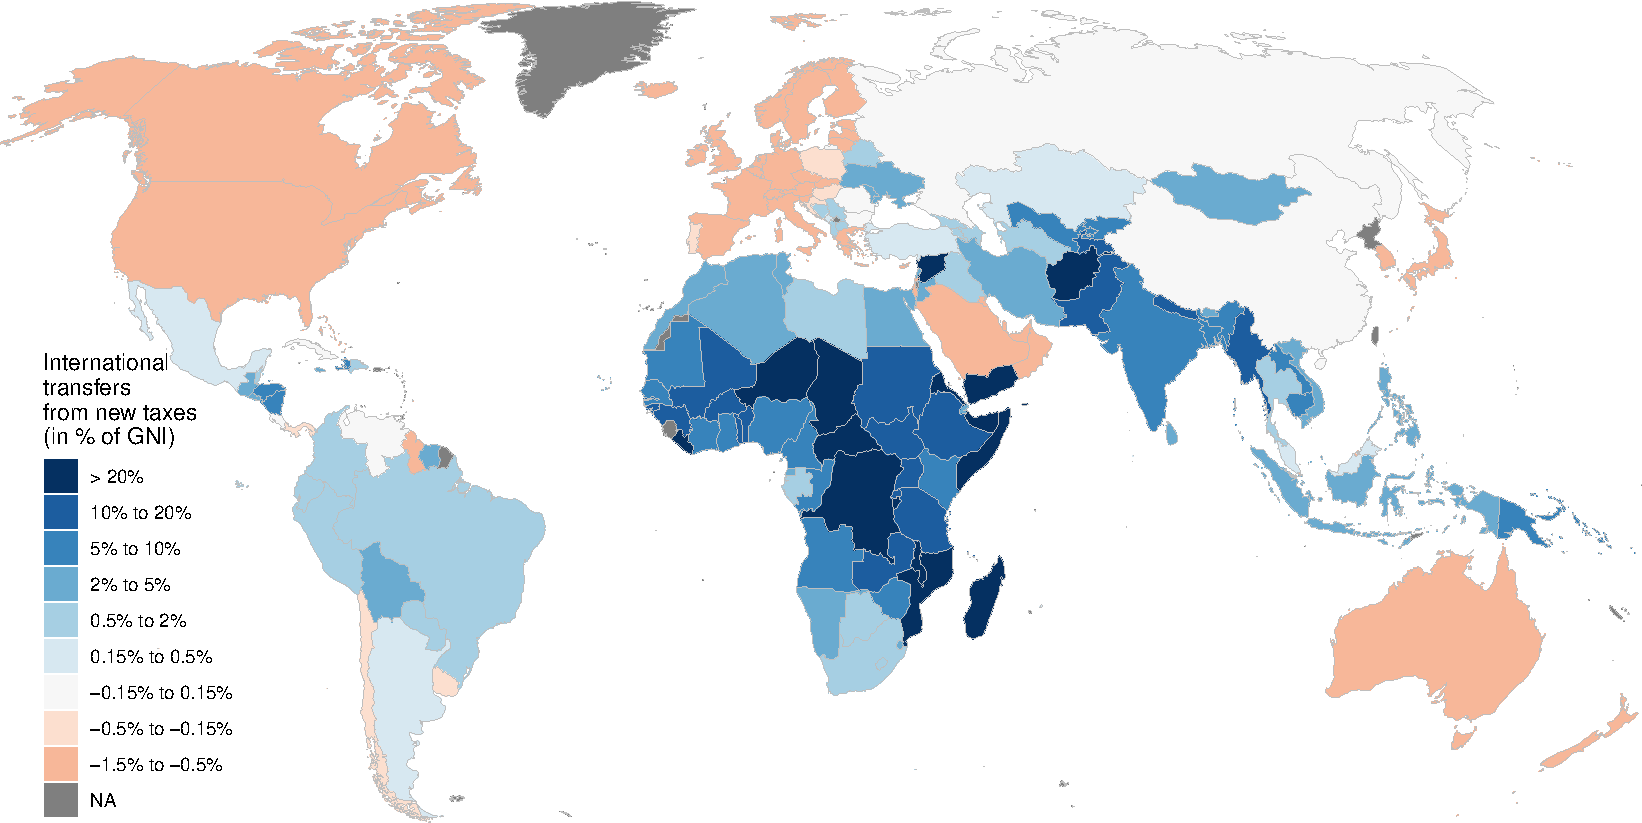
\includegraphics[width=1\textwidth]{../figures/maps/net_gain_over_gdp_both_taxes_pop.pdf}} 
\end{figure}

\begin{figure}[h!] 
  \caption{Net gain for state budgets from new taxes and international transfers (revenue plus net transfer).}\label{fig:budget_gain_both_taxes}
  \makebox[\textwidth][c]{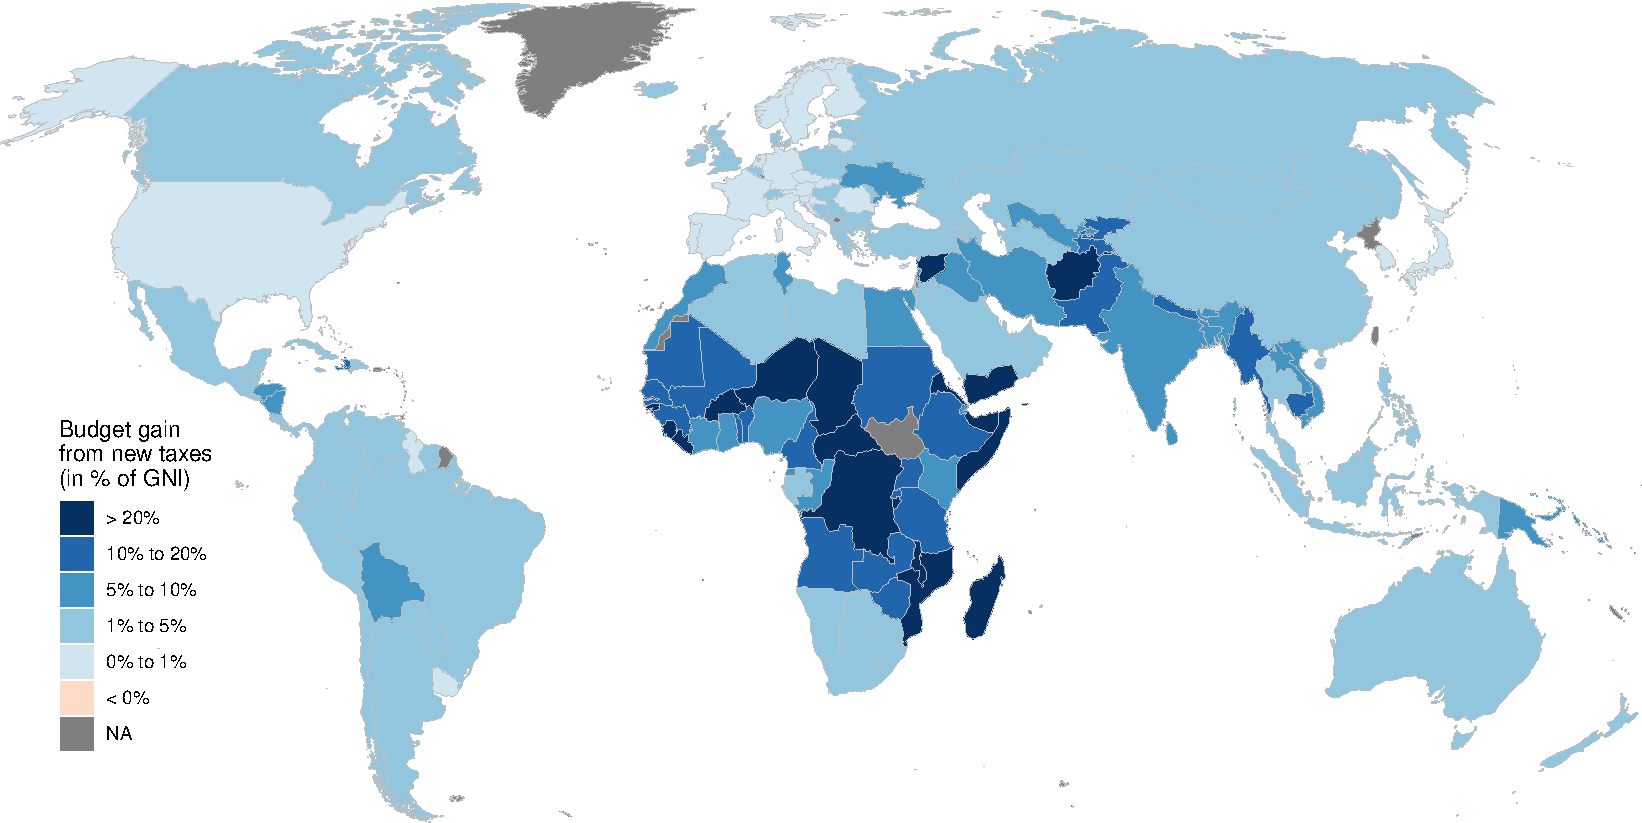
\includegraphics[width=.95\textwidth]{../figures/maps/budget_gain_over_gdp_both_taxes_pop.pdf}} 
\end{figure}


% \subsection{The advantages of a Sustainable Union\label{subsec:advantages}}



% III. sustainable union: stronger incentive for LMIC to join; can simplify allocation (transfers purely based on GNI); count anti-climate legislation as negative contributions; 
% TODO explain treaty; 
% distributive effects.

% Conclusion: What next? Scientific council to conduct in-depth analyses and answer to countries' questions
% stronger incentive for LMIC to join; can simplify allocation (transfers purely based on GNI)

\clearpage
\renewcommand{\url}[1]{\href{#1}{Link}} % NCCcomment
\bibliographystyle{plainnaturl_clean} % NCCcomment
\bibliography{global_tax_attitudes}

\appendix

% \section{The draft treaty} % TODO!

% Annex: Treaty/ies

% Difficult to reconcile:
% 1. countries pay marginal footprint to RoW at universal eq price
% 2. submedial countries are not net contributor in partial union (they lose when price=floor if their planned emissions > rights * club/world average ~ rights * 3/4, when club's rights sum to equal pc). Can be presented as ~1.5°C trajectory with extra rights for submedial or ~1.8°C trajectory with less rights for poor and rich.
% 3. no discontinuity in price/transfers when union expands (so that members have interest in expansion)

% Options:
% a. difference between universal and union eq price is collected/recycled nationally for C-submedial countries and the share over the global average is transferred to submedial countries for supermedial ones. Fails 1,2,3.
%>b. transfers are unrelated to emissions, based on GNI. Fails 1.
% c. transfers based on GNI + departure from expected emissions reductions. May fail 2.
% d. union price is universal eq, extra transfers for submedial countries (to the expense of high and low income ones). Fails 3.
% e. countries with GNI pc < 1.5 average can opt out from revenue sharing. Fails 1 (and rights left to others unpredictable).
% f. keep carbon price floor low. Fails 3, also 2 but mitigated.
%>g. revenue share of surmedial LMIC augmented by their footprint/club average at t=0. Fails 2 to the extend emissions decrease slower than in the rest of the club. 
%>h. Differentiated rights + high price floor. May fail 2 (if differentiated prices don't accommodate enough departure, i.e. if AFR doesn't renounce to enough of its rights).
%>>i No price floor (except for countries who repeal climate laws), MIC rights get as much rights as their needs. Fails 1 (equivalent to higher temperature target), 3 (same issue with Sustainable Union). 
%>j A price (rather than quantity) target with equal pc sharing except for countries < 1.2 average GDP which can be exempted from revenue sharing (with phase out up to 1.5 average) and rule to avoid HIC being net receiver => clear, rule-based, only issue is that price may be too low; and if automatically increased then too big an advantage for exempted countries as they increase emissions without increasing transfers (i.e. fails 1 for exempted countries => could be avoided by adding payments if departure from expected emissions reductions) TODO give this as alternative

% Pq je suis passé de GCP à FFU? 1. pour ne plus dire que EU perd (mais j'peux parler de droits équivalents dans GCP), 2. pour donner de la flexibilité sur les departures (par ex éviter de donner un avantage trop grand à la Chine, qui va se décarboner plus vite que le club) et sur la répartition temporelle (donner plus tard à Inde pour éviter qu'elle ne sorte), 3. parce que je renonçais à un prix conséquent les premières années (hot air)
% Pb de FFU: la répartition temporelle des droits doit tenir compte du prix plancher, qui n'est pas connu (participation partielle induit différence distributive par rapport à simple marché). => fixer le prix (en fonction de qui participe)
% Avantages du GCP? 1. permet un prix plus élevé au début car les surmédiaux sont ajustés relativement à moyenne du club et pas moyenne mondiale comme ds FFU (il le faut pour éviter une augmentation trop rapide lorsque le marché devient binding ou si US rejoignent), 2. rule-based plutôt que discretionary, 3. permet de s'ajuster aux circonstances changeantes (par ex si Chine a rattrapé EU en PIB/hab), 

% Ask to each country: Imagine int'l ETS (membership, price unknown, though probably just Global South, no price floor): 
% How much allowances they would want? (minimum acceptable, fair, ideal number; give justification for each)
% Total/world allowances they would want until net zero (minimum, ideal, maximum).
% Allocation rules they'd accept: equal pc, cumulative equal pc, CC, BAU for MIC, grandfathering
% => work out a solution based on the answers

% - Pricing:
% -- equivalence differentiated prices - rights but uniform price better, countries can always add policies to e.g. subsidize fuels if they wish
% -- for acceptability + fairness, we need departures from equal pc
% -- simulations using NICE
% -- feasibility of global redistributive policy: surveys, informal support of diplomats (even EU saying govts is pb, they personally like)

% Start paper on Fossil-Free Union, then expand.

% Argue in favor of FFU: guarantee the union respects its targets; determines burden sharing.
% Carbon price floors very important as it's binding in first years. Must be complemented by the obligation to pay higher price if country reduces its domestic carbon price / climate regulations. In effect, acts as a generalized JTEP (more favorable to LDCs). 

% PB of FFU: in first phase with carbon price floor, China loses as it has less rights among the union than its emissions share in the union. => No, I think it's been computed so that China doesn't lose. The above effect is mitigated by the carbon trade + larger rights.
% PB of SU: same issue if partial participation => No because China is allowed to skip the redistribution part and just apply the FFU.
% => Think of treaty rules
% Le prix plancher doit correspondre au prix qui serait atteint en cas de participation universelle, pour qu'il y ait suffisamment de réductions d'émission, de transferts, et que les états membres n'aient pas un désintérêt à ce que les US joignent

% Pb du FFU: EU has no financial interest that US joins (as long as EU is a net contributor => determine loss of EU when US joins; determine date of US joining that makes EU indifferent). Indeed, EU pays price*(emissions - rights). If US joins, price will increase and (e - r) be constant. If instead of fixing the rights we fixed the price, EU would have interest that US joins, as its rights (equal to union average) would increase. EU would also have interest of US joining in the case 1% GNI return in fct of pop.
% => What rules leave no one worse off when big emitters join? What rules leave big emitters indifferent when bigger emitters join?

% Global policies to phase out fossil fuels 
% - Principles: non-universal, open, redistributive, non-dichotomic
% - Climate justice -> justice (burden-sharing options, criticism of CERF, grandfathering would be plausible in absence of broader inequality/justice hence can make sense within country)
% - Finance options (multilateral guarantees, climate bonds, money creation - Dafermos...)
% - Common standards (ships, cars, banning coal or oil exploration)
% - Supply-side policies (critique of fossil non proliferation)
% - Pricing:
% -- equivalence differentiated prices p_i = p + a_i where mean(p_i)=p  and differentiated rights per capita r_i : r_i = p*e - a_i*e_i, where e_i is country's emission pc and e global average.
% -- uniform price better, countries can always add policies to e.g. subsidize fuels if they wish
% -- for acceptability + fairness, we need departures from equal pc
% -- simulations using NICE
% -- critiques of other proposals: Pezsko, Edenhofer, Nordhaus, Piketty, rationing, proposals lacking sectoral coverage (CBAM sectors) or redistribution (restricting ITMOs to high-integrity countries)...
% -- feasibility of global redistributive policy: surveys, informal support of diplomats (even EU saying govts is pb, they personally like)
% -- call for expert contributions and common proposal

% \begin{figure}[b!]
%   \caption[Title.]{Caption
%   }\label{fig:antipoverty_tax_7}
%   \makebox[\textwidth][c]{\includegraphics[width=\textwidth]
%   {../figures/antipoverty_2_tax_7_average.pdf}}
% \end{figure}

% \begin{figure}[h!]
%     \caption[Title.]{Caption.}\label{fig:kenya}
%   \begin{subfigure}{.5\textwidth}
%     \caption[]{Caption_a.}\label{fig:kenya_policies}
%     \includegraphics[width=\textwidth]{../figures/Kenya_policies.pdf}
%   \end{subfigure} \;
%   \begin{subfigure}{.5\textwidth}
%     \caption[]{Caption_b.}\label{fig:kenya_cap}
%     \includegraphics[width=\textwidth]{../figures/Kenya_cap.pdf}
%   \end{subfigure}
%   \\ \quad \\
%   \begin{subfigure}{.5\textwidth}
%     \caption[]{Caption_c.}\label{fig:kenya_tax}
%     \includegraphics[width=\textwidth]{../figures/Kenya_tax.pdf}
%   \end{subfigure} \;
%   \begin{subfigure}{.5\textwidth}
%     \caption[]{Caption_d.}\label{fig:kenya_floor}
%     \includegraphics[width=\textwidth]{../figures/Kenya_floor.pdf}
%   \end{subfigure}
% \end{figure}  


% \section{Discussion\label{sec:conclusion}} 

% \begin{methods}  % WPcomment
  \begin{small} % NCCcomment
% \section*{\normalsize Data and code availability}

% \end{methods} % WPcomment
\end{small}  % NCCcomment

% \theendnotes

% \clearpage
\section{Raw results% from the complementary surveys
}\label{app:raw_results}
% /!\ Do not replace by app_desc_stats_US1 as the latter also contains figures that are already in the main text

Country-specific raw results are also available as supplementary material files:  \href{https://github.com/bixiou/global_tax_attitudes/raw/main/paper/app_desc_stats_US.pdf}{US}, \href{https://github.com/bixiou/global_tax_attitudes/raw/main/paper/app_desc_stats_EU.pdf}{EU}, \href{https://github.com/bixiou/global_tax_attitudes/raw/main/paper/app_desc_stats_FR.pdf}{FR}, \href{https://github.com/bixiou/global_tax_attitudes/raw/main/paper/app_desc_stats_DE.pdf}{DE}, \href{https://github.com/bixiou/global_tax_attitudes/raw/main/paper/app_desc_stats_ES.pdf}{ES}, \href{https://github.com/bixiou/global_tax_attitudes/raw/main/paper/app_desc_stats_UK.pdf}{UK}.

\begin{figure}[h!]
    \caption[Absolute support for global climate policies]{Absolute support for global climate policies. \\ Share of \textit{Somewhat} or \textit{Strongly support} (in percent, $n$ = 40,680). The color blue denotes an absolute majority. See Figure \ref{fig:oecd} for the relative support. (Questions \ref{q:scale}-\ref{q:millionaire_tax})} 
    \makebox[\textwidth][c]{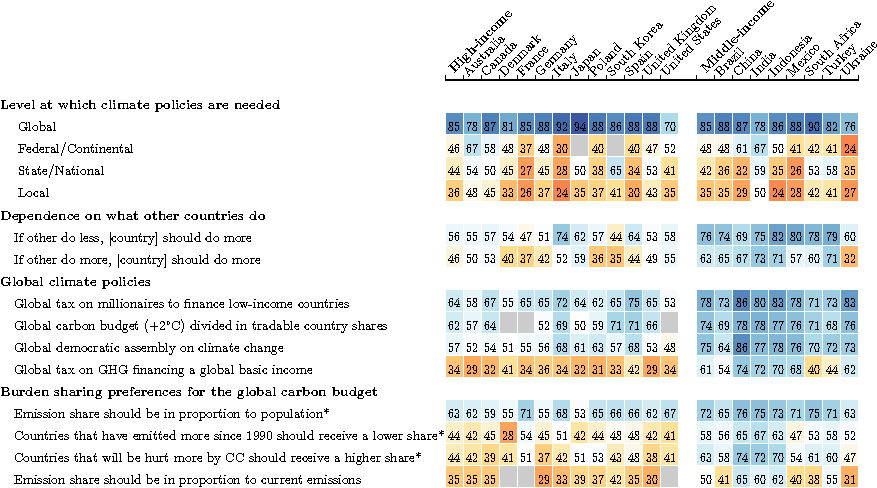
\includegraphics[width=1.2\textwidth]{../figures/OECD/Heatplot_burden_share_all_positive_countries.pdf}}\label{fig:oecd_absolute}
    {\footnotesize *In Denmark, France and the U.S., the questions with an asterisk were asked differently, cf. Question \ref{q:burden_sharing_asterisk}. } 
\end{figure}

\begin{figure}[h!]
    \caption[Comprehension]{Correct answers to comprehension questions (in percent). (Questions \ref{q:understood_gcs}-\ref{q:understood_both})}\label{fig:understood_each}
    \makebox[\textwidth][c]{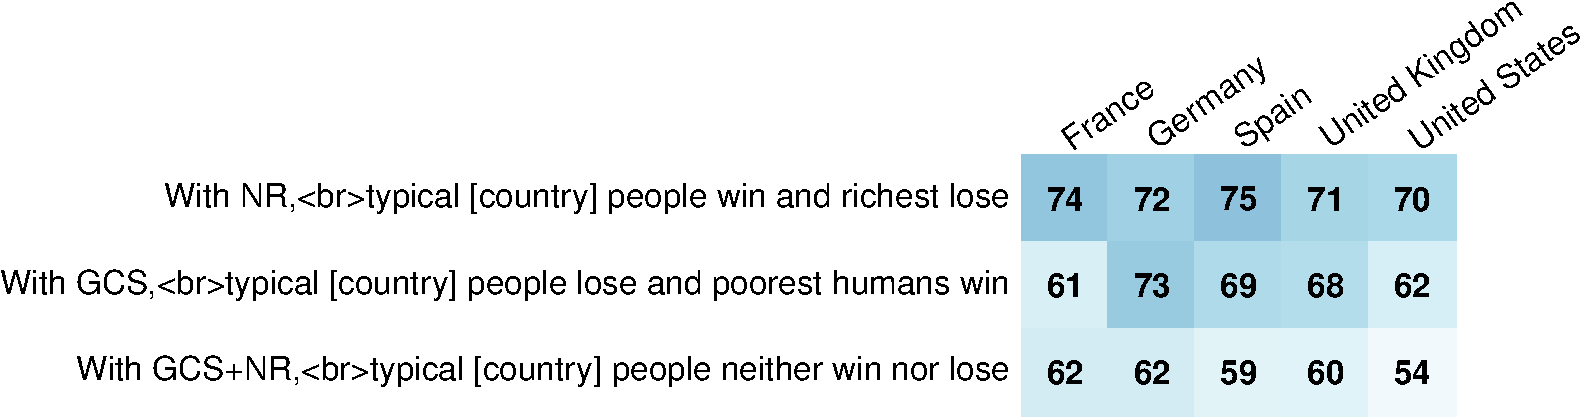
\includegraphics[width=\textwidth]{../figures/country_comparison/understood_each_positive.pdf}} 
\end{figure}

\begin{figure}[h!]
    \caption[Comprehension score]{Number of correct answers to comprehension questions (mean). (Questions \ref{q:understood_gcs}-\ref{q:understood_both})}\label{fig:understood_score}
    \makebox[\textwidth][c]{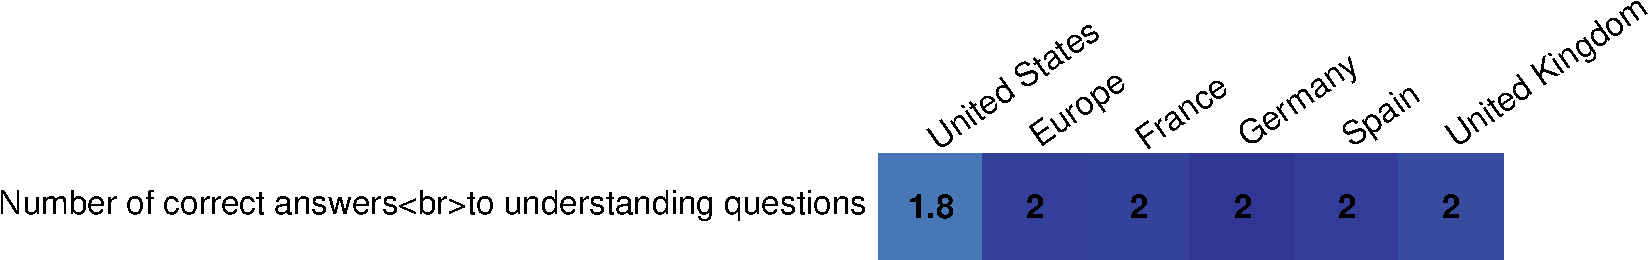
\includegraphics[width=\textwidth]{../figures/country_comparison/understood_score_mean.pdf}} 
\end{figure}

% \begin{figure}[h!]
%     \caption[Support for the Global Climate Scheme]{Support for the GCS, NR and the combination of GCS, NR and C. (Questions \ref{q:gcs_support}, \ref{q:nr_support} and \ref{q:crg_support})}\label{fig:support_binary}
%     \makebox[\textwidth][c]{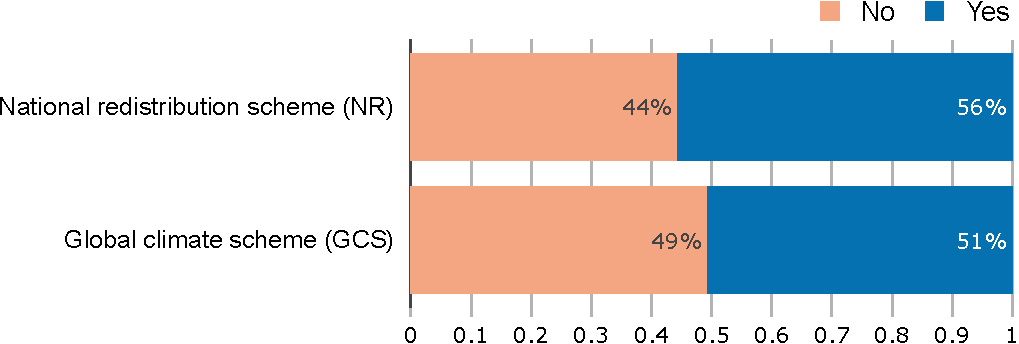
\includegraphics[width=.9\textwidth]{../figures/country_comparison/support_binary.pdf}} 
% \end{figure}

% \begin{figure}[h!]
%     \caption[Beliefs about support for the GCS and NR]{Beliefs regarding the support for the GCS and NR. (Questions \ref{q:gcs_belief} and \ref{q:nr_belief})}\label{fig:belief}
%     \makebox[\textwidth][c]{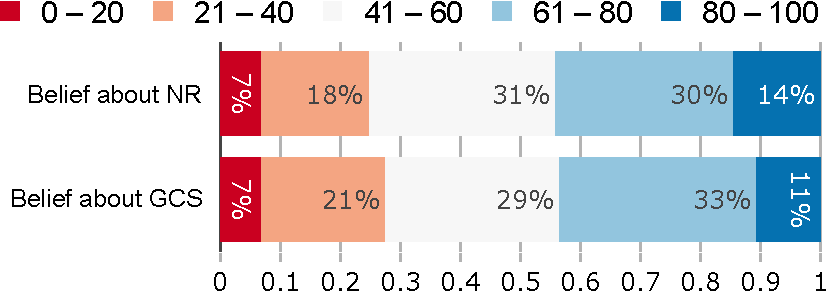
\includegraphics[width=.8\textwidth]{../figures/country_comparison/belief.pdf}} 
% \end{figure}

\begin{figure}[h!]
    \caption[List experiment]{List experiment: mean number of supported policies. (Section \ref{subsubsec:list_exp}, Question \ref{q:list_exp})}\label{fig:list_exp}
    \makebox[\textwidth][c]{
\includegraphics[width=.7\textwidth]{../figures/country_comparison/list_exp_mean.pdf}} 
\end{figure}

\begin{figure}[h!]
    \caption[Conjoint analyses 1 and 2]{Conjoint analyses 1 and 2. (Section \ref{subsubsec:conjoint}, Questions \ref{q:conjoint_a}-\ref{q:conjoint_b})}\label{fig:conjoint}
    \makebox[\textwidth][c]{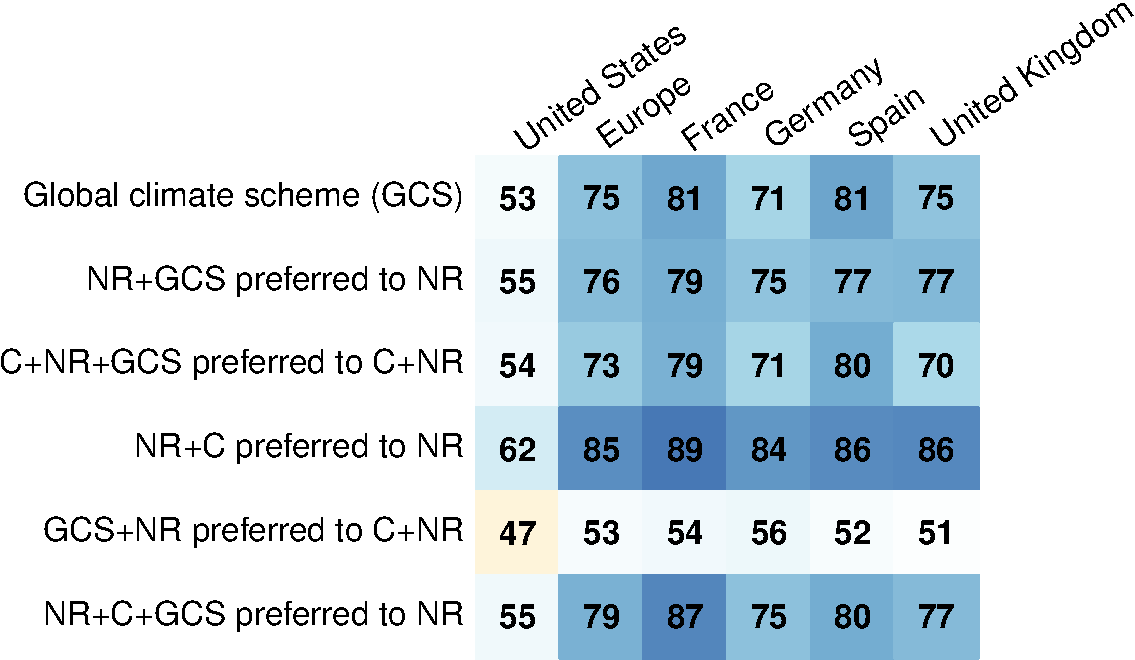
\includegraphics[width=.8\textwidth]{../figures/country_comparison/conjoint_ab_all_positive.pdf}} 
\end{figure}

% \begin{figure}[h!] % already in text
%     \caption{[Asked only to non-Republicans] Conjoint analysis n°4: random programs at the Democratic primary. (Question \ref{q:conjoint_r})}\label{fig:ca_r}
%     \makebox[\textwidth][c]{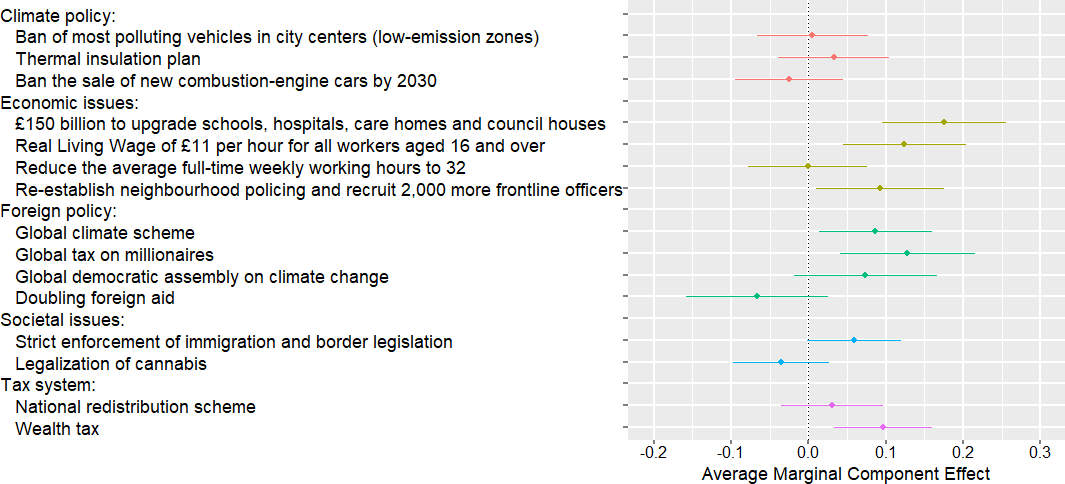
\includegraphics[width=\textwidth]{../figures/country_comparison/ca_r.png}} 
% \end{figure}

% \begin{figure}[h!]
%     \caption[Influence of the GCS on preferred platform]{Influence of the GCS on preferred platform:\\ Preference for a random platform A that contains the Global Climate Scheme rather than a platform B that does not (in percent). (Question \ref{q:conjoint_d}; in the U.S., asked only to non-Republicans.)}\label{fig:conjoint_left_ag_b}
%     \makebox[\textwidth][c]{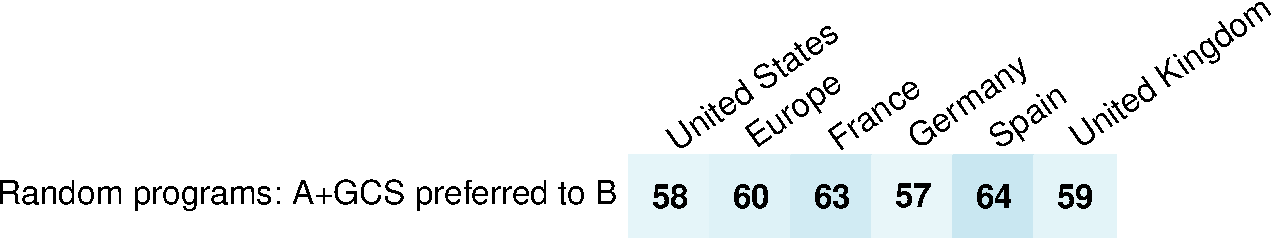
\includegraphics[width=\textwidth]{../figures/country_comparison/conjoint_left_ag_b_binary_positive.pdf}} 
% \end{figure}

\begin{figure}[h!]
    \caption[Perceptions of the GCS]{Perceptions of the GCS. Elements seen as important for supporting the GCS in a 4-Likert scale (in percent). (Question \ref{q:gcs_important})}\label{fig:gcs_important}
    \makebox[\textwidth][c]{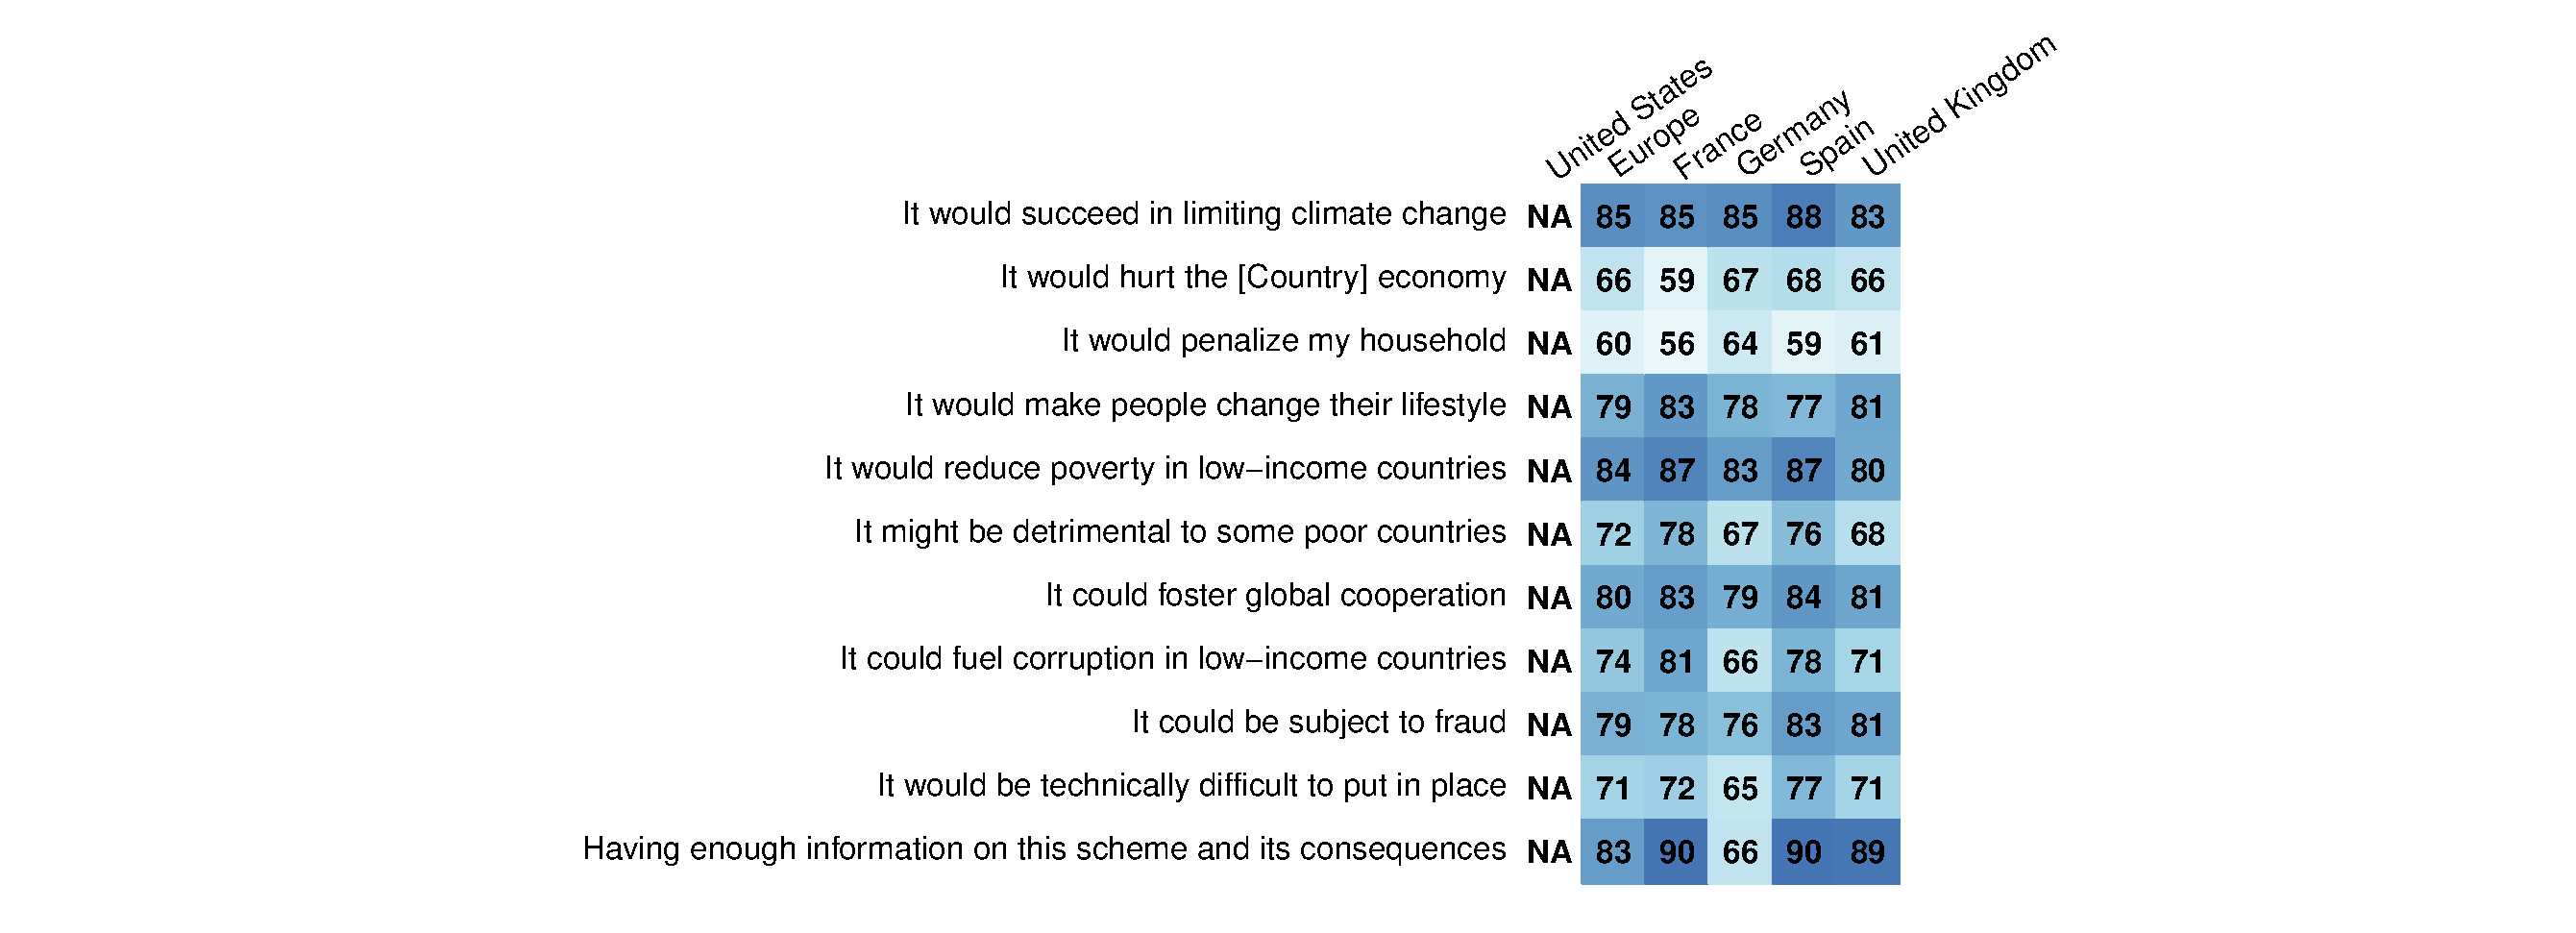
\includegraphics[width=\textwidth]{../figures/country_comparison/gcs_important_positive.pdf}} 
\end{figure}

\begin{figure}[h!]
    \caption[Classification of open-ended field on the GCS]{Perceptions of the GCS. Elements found in the open-ended field on the GCS (manually recoded, in percent). (Question \ref{q:gcs_field})}\label{fig:gcs_field}
    \makebox[\textwidth][c]{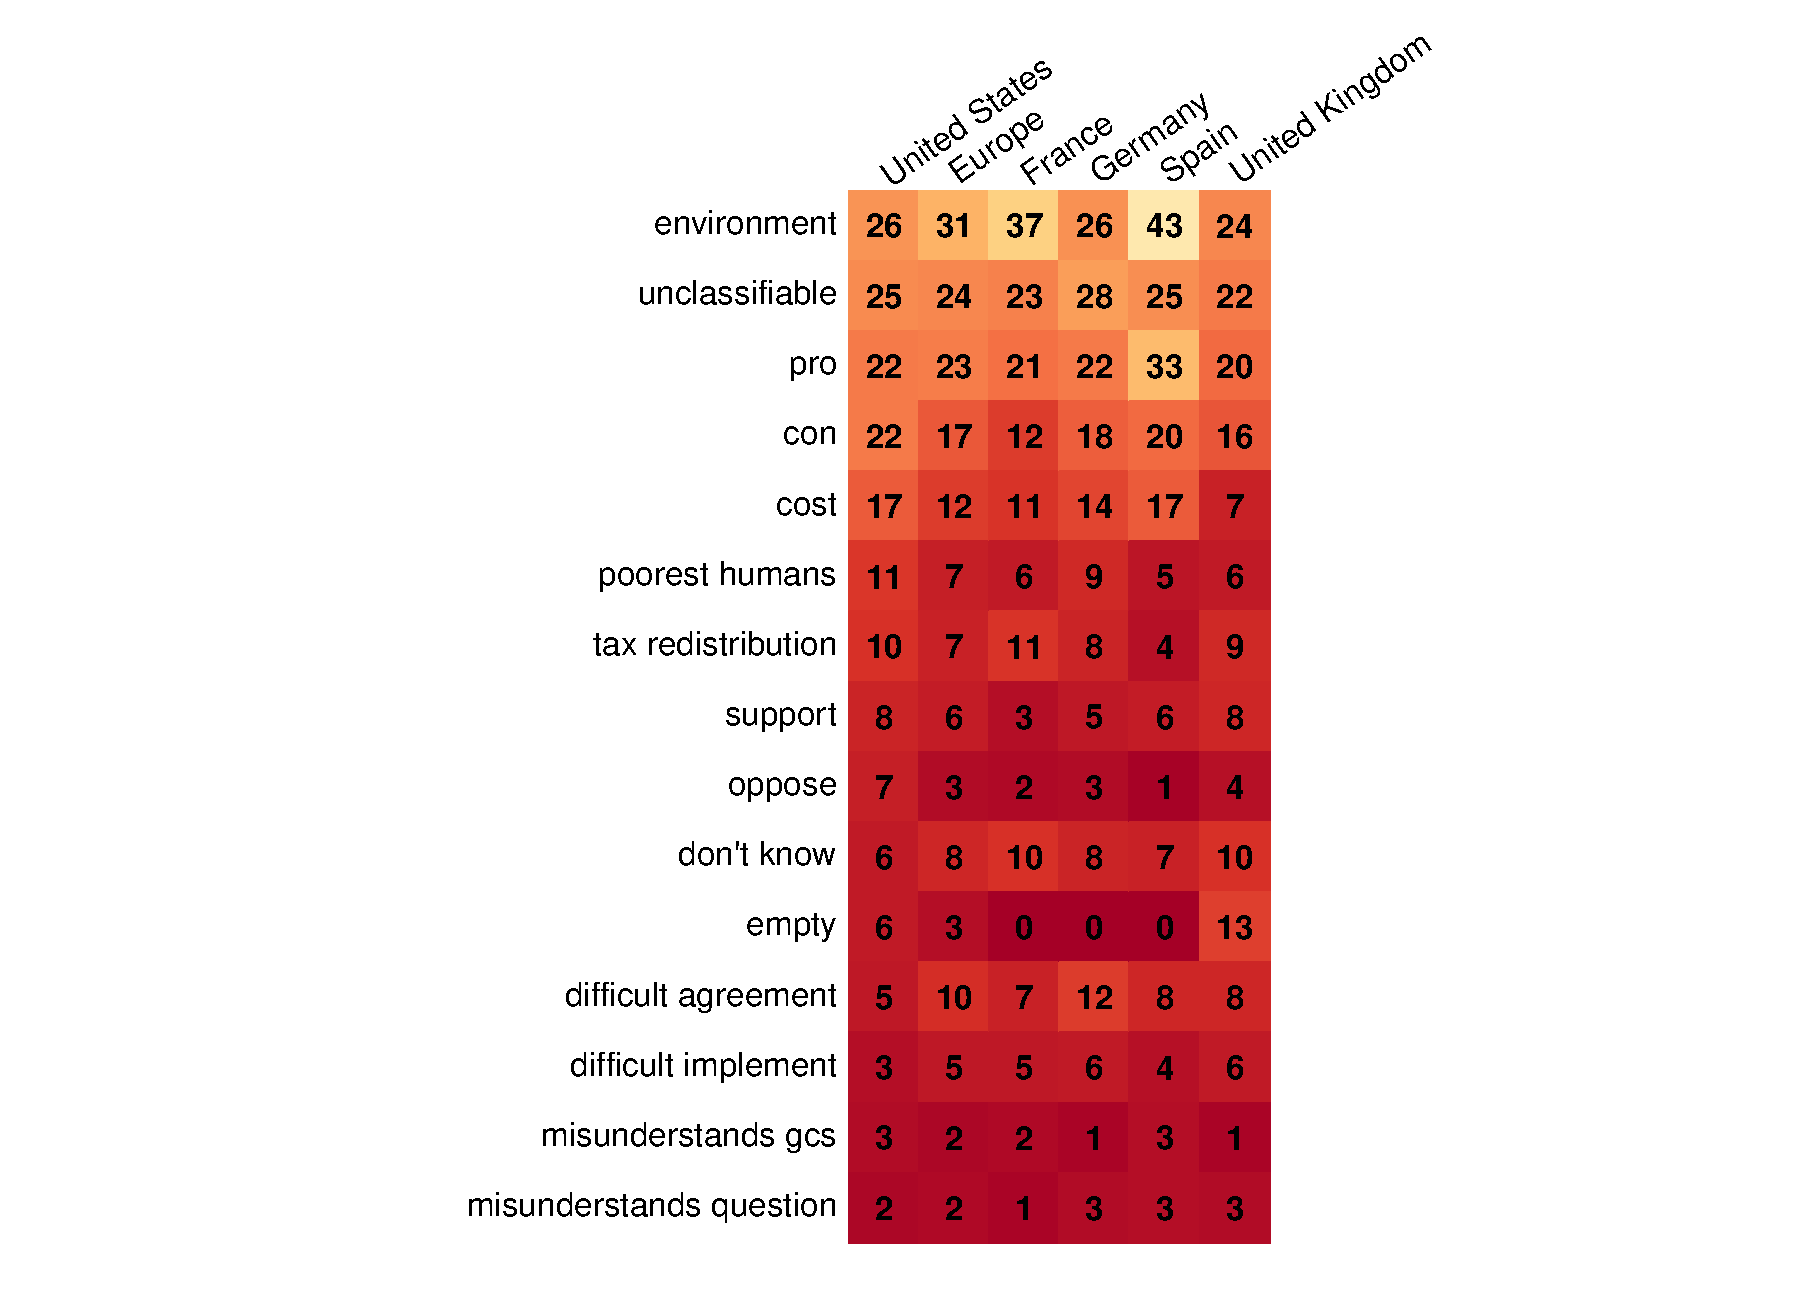
\includegraphics[width=.75\textwidth]{../figures/country_comparison/gcs_field_positive.pdf}} 
\end{figure}

\begin{figure}[h!]
    \caption[Topics of open-ended field on the GCS]{Perceptions of the GCS. Keywords found in the open-ended field on the GCS (automatic search ignoring case, in percent). (Question \ref{q:gcs_field})}\label{fig:gcs_field_contains}
    \makebox[\textwidth][c]{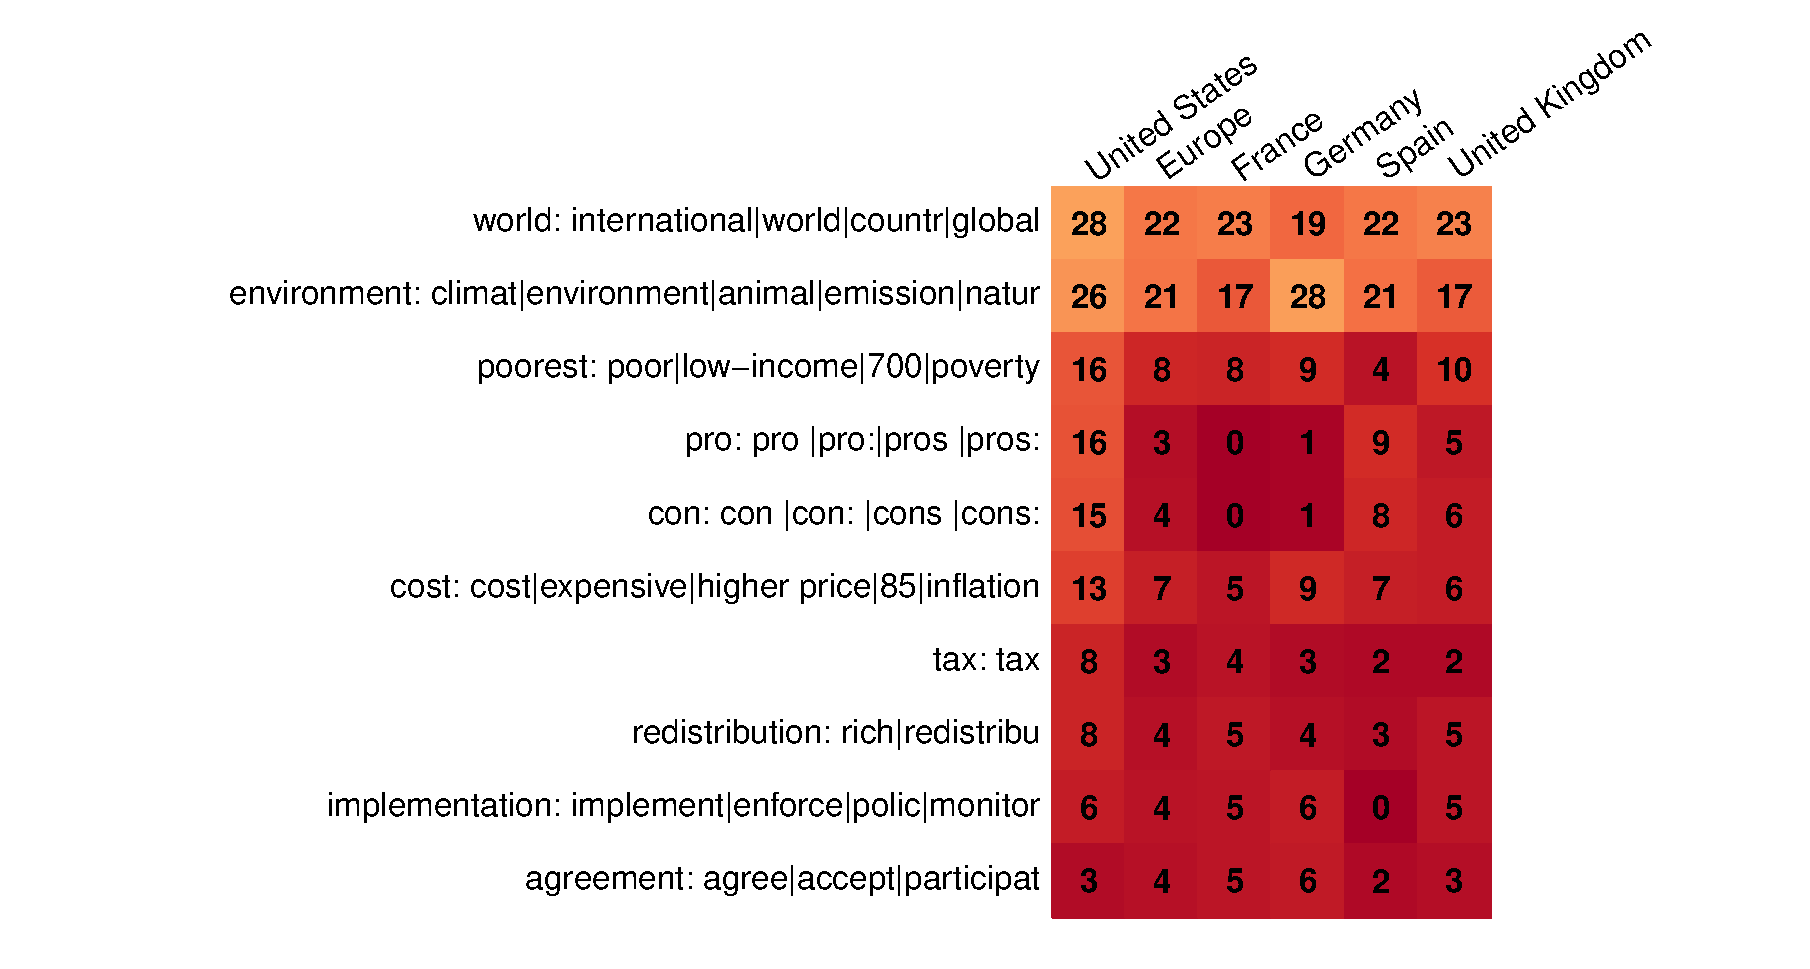
\includegraphics[width=\textwidth]{../figures/country_comparison/gcs_field_contains_positive.pdf}} 
\end{figure}

\begin{table}[h]\label{tab:branch_gcs}
    \caption[Campaign and bandwagon effects on the support for the GCS.]{Effects on the support for the GCS of a question on its pros and cons and on information about the actual support, in the U.S. (See Section \ref{subsec:questionnaire_perceptions} in the US2 Questionnaire)} 
    \makebox[\textwidth][c]{
        
\begin{tabular}{@{\extracolsep{5pt}}lcccc} 
\\[-1.8ex]\hline 
\hline \\[-1.8ex] 
 & \multicolumn{4}{c}{Support} \\ 
\cline{2-5} 
\\[-1.8ex] & \multicolumn{2}{c}{Global Climate Scheme} & \multicolumn{2}{c}{National Redistribution} \\ 
\\[-1.8ex] & (1) & (2) & (3) & (4)\\ 
\hline \\[-1.8ex] 
Control group mean & 0.557 & 0.557 & 0.569 & 0.569  \\ \hline \\[-1.8ex]
 Treatment: Open\mbox{-}ended field on GCS pros \& cons & $-$0.073$^{**}$ & $-$0.071$^{**}$ & $-$0.035 & $-$0.030 \\ 
  & (0.035) & (0.031) & (0.035) & (0.032) \\ 
  Treatment: Closed questions on GCS pros \& cons & $-$0.109$^{***}$ & $-$0.096$^{***}$ & $-$0.065$^{*}$ & $-$0.062$^{**}$ \\ 
  & (0.034) & (0.031) & (0.034) & (0.031) \\ 
  Treatment: Info on actual support for GCS and NR & $-$0.021 & $-$0.015 & 0.048 & 0.056$^{*}$ \\ 
  & (0.034) & (0.031) & (0.033) & (0.031) \\ 
 \hline \\[-1.8ex] 
Includes controls &  & \checkmark &  & \checkmark \\

Observations & 2,000 & 1,995 & 2,000 & 1,995 \\ 
R$^{2}$ & 0.007 & 0.170 & 0.007 & 0.154 \\ 
\hline 
\hline \\[-1.8ex] 
\end{tabular} 
    }
    {\footnotesize %\textit{Note}: 
    }
\end{table}

\begin{figure}[h!]
    \caption[Donation to Africa vs. own country]{Donation in case of lottery win, depending on the recipient's (randomly drawn) nationality (mean). (Question \ref{q:donation})}\label{fig:donation}
    \makebox[\textwidth][c]{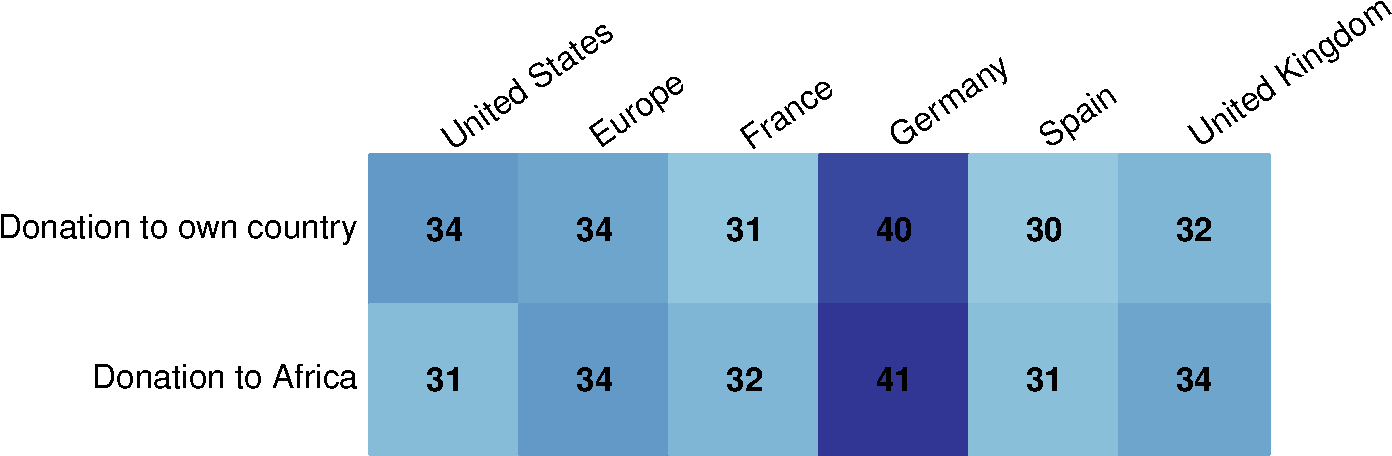
\includegraphics[width=.8\textwidth]{../figures/country_comparison/donation_mean.pdf}} 
\end{figure}

\begin{figure}[h!]
    \caption[Support for a global wealth tax]{Support for a global wealth tax. \\
    ``Do you support or oppose a tax on millionaires of all countries to finance low-
    income countries? \\
    Such tax would finance infrastructure and public services such as access to drinking water, healthcare, and education.'' (Question \ref{q:global_tax})}\label{fig:global_tax}
    \makebox[\textwidth][c]{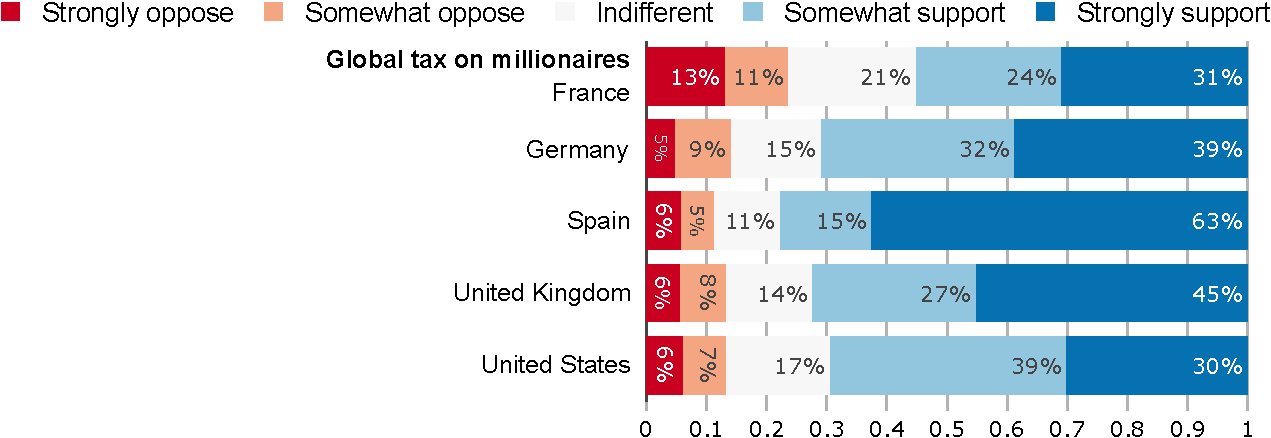
\includegraphics[width=\textwidth]{../figures/country_comparison/global_tax_support.pdf}} 
\end{figure}

\begin{figure}[h!]
    \caption[Support for a national wealth tax]{Support for a national wealth tax financing public services like healthcare, education, and social housing. (Question \ref{q:national_tax})}\label{fig:national_tax}
    \makebox[\textwidth][c]{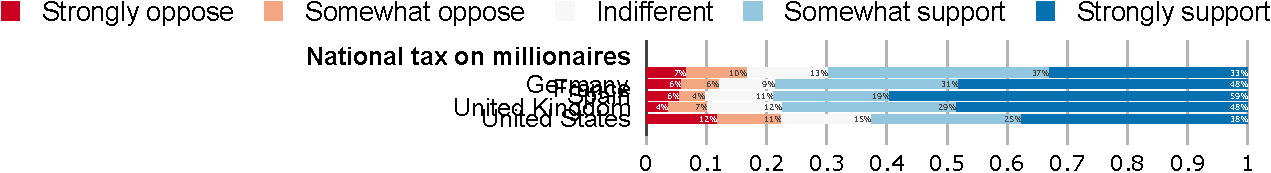
\includegraphics[width=\textwidth]{../figures/country_comparison/national_tax_support.pdf}} 
\end{figure}

\begin{figure}[h!]
    \caption[Preferred share of global tax for low-income countries]{Preferred share of global wealth tax revenues that should be pooled to finance low-income countries. (Question \ref{q:global_tax_global_share})}\label{fig:global_tax_global_share}
    \makebox[\textwidth][c]{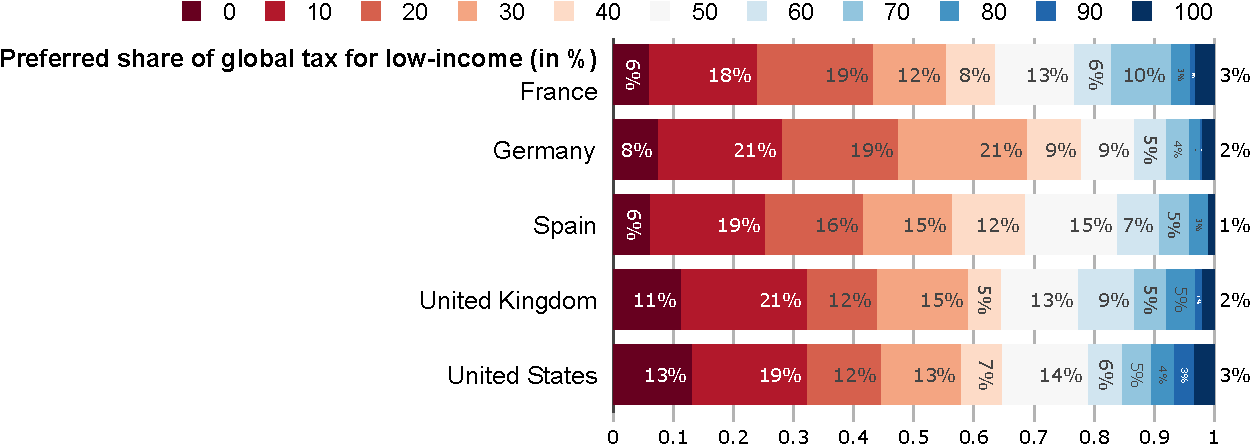
\includegraphics[width=\textwidth]{../figures/country_comparison/global_tax_global_share.pdf}} 
\end{figure}

\begin{figure}[h!]
    \caption[Support for sharing half of global tax revenues with low-income countries]{Support for sharing half of global tax revenues with low-income countries, rather that each country retaining all the revenues it collects (in percent). (Question \ref{q:global_tax_sharing})}\label{fig:global_tax_sharing}
    \makebox[\textwidth][c]{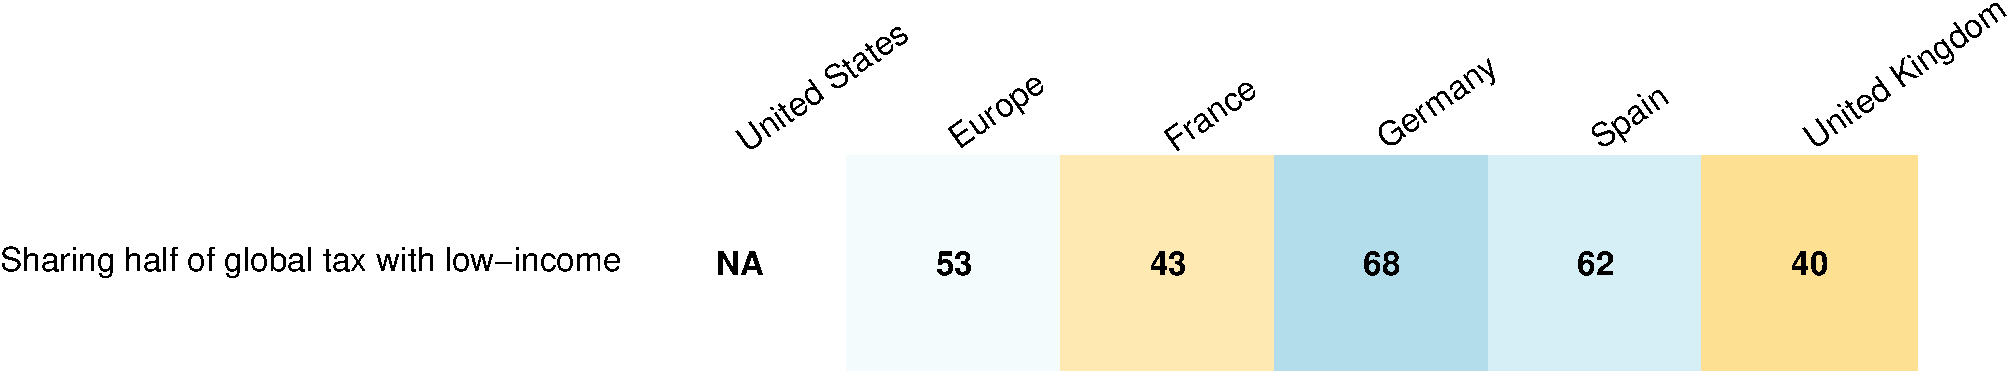
\includegraphics[width=\textwidth]{../figures/country_comparison/global_tax_sharing_positive.pdf}} 
\end{figure}

\begin{figure}[h!]
    \caption[Perceived foreign aid]{Perceived foreign aid. ``From your best guess, what percentage of [own country] government spending is allocated to foreign aid (that is, to reduce poverty in low-income countries)?'' (Question \ref{q:foreign_aid_belief})}\label{fig:foreign_aid_belief}
    \makebox[\textwidth][c]{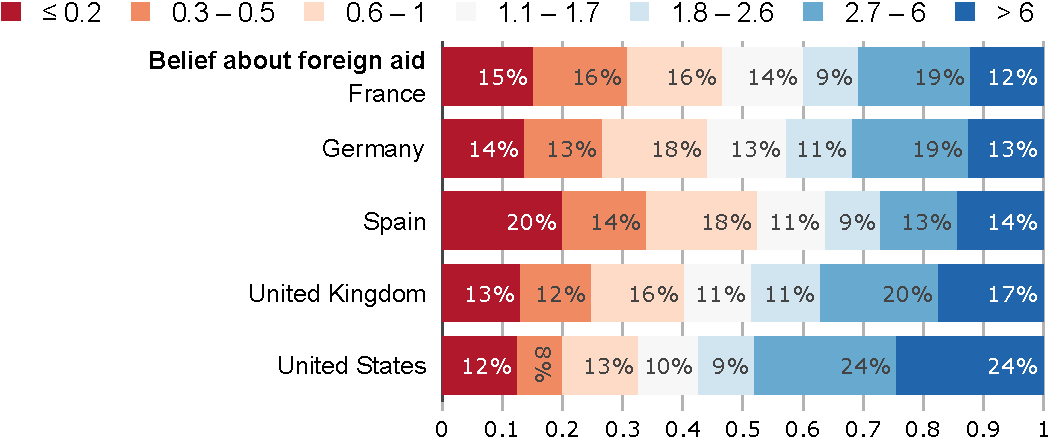
\includegraphics[width=\textwidth]{../figures/country_comparison/foreign_aid_belief_agg.pdf}} 
\end{figure}

\begin{figure}[h!]
    \caption[Preferred foreign aid (without info on actual amount)]{Preferred foreign aid (without info on actual amount). \\ ``If you could choose the government spending, what percentage would you allocate
    to foreign aid?'' (Question \ref{q:foreign_aid_preferred})}\label{fig:foreign_aid_preferred_no_info}
    \makebox[\textwidth][c]{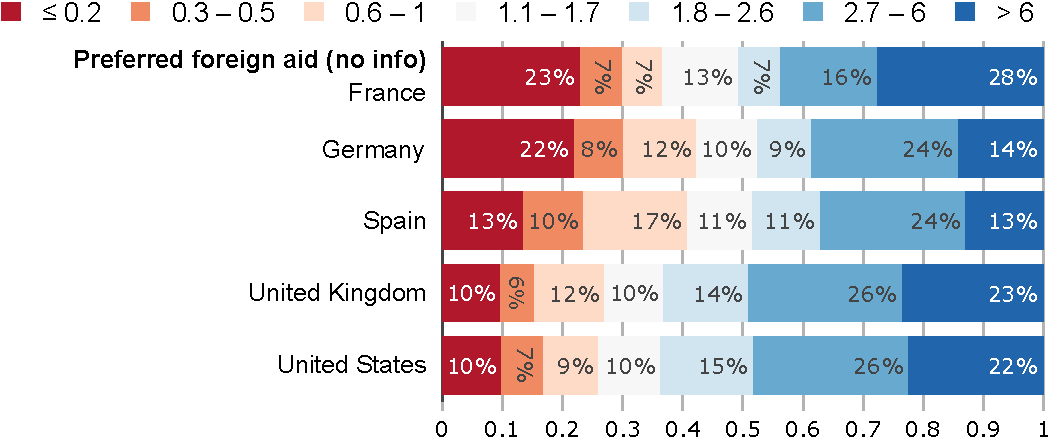
\includegraphics[width=\textwidth]{../figures/country_comparison/foreign_aid_preferred_no_info_agg.pdf}} 
\end{figure}

\begin{figure}[h!]
    \caption[Preferred foreign aid (after info on actual amount)]{Preferred foreign aid (after info on actual amount). \\ ``Actually,
    [US1: 0.4\%; FR: 0.8\%; DE: 1.3\%; ES: 0.5\%; UK: 1.7\%] of [own country] government spending is allocated to foreign aid. \\
    If you could choose the government spending, what percentage would you allocate
    to foreign aid?'' (Question \ref{q:foreign_aid_preferred})}\label{fig:foreign_aid_preferred_info}
    \makebox[\textwidth][c]{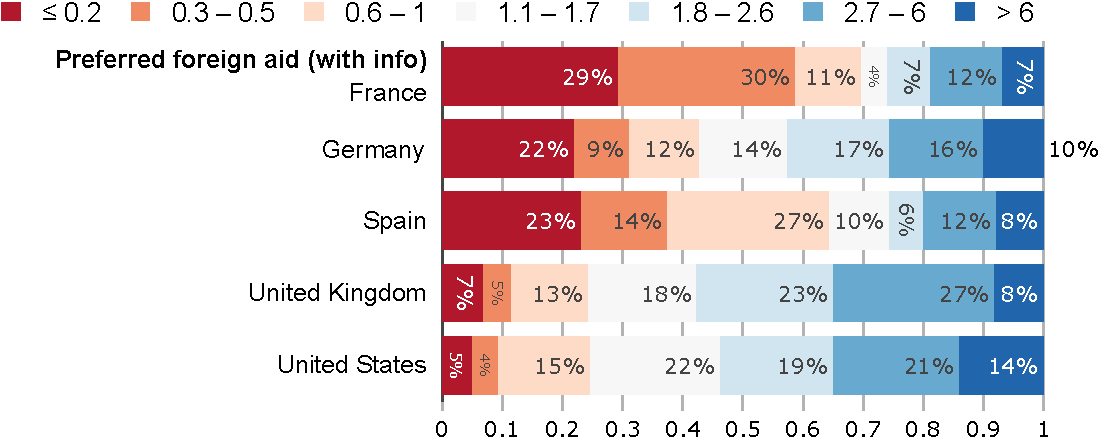
\includegraphics[width=\textwidth]{../figures/country_comparison/foreign_aid_preferred_info_agg.pdf}} 
\end{figure}

\begin{figure}[h!]
    \caption[Preferences for funding increased foreign aid]{Preferences for funding increased foreign aid. [Asked iff preferred foreign aid is strictly greater than [Info: actual; No info: perceived] foreign aid] \\ ``How would you like to finance such increase in foreign aid? (Multiple answers possible)'' (in percent) (Question \ref{q:foreign_aid_raise_how})}\label{fig:foreign_aid_raise_how}
    \makebox[\textwidth][c]{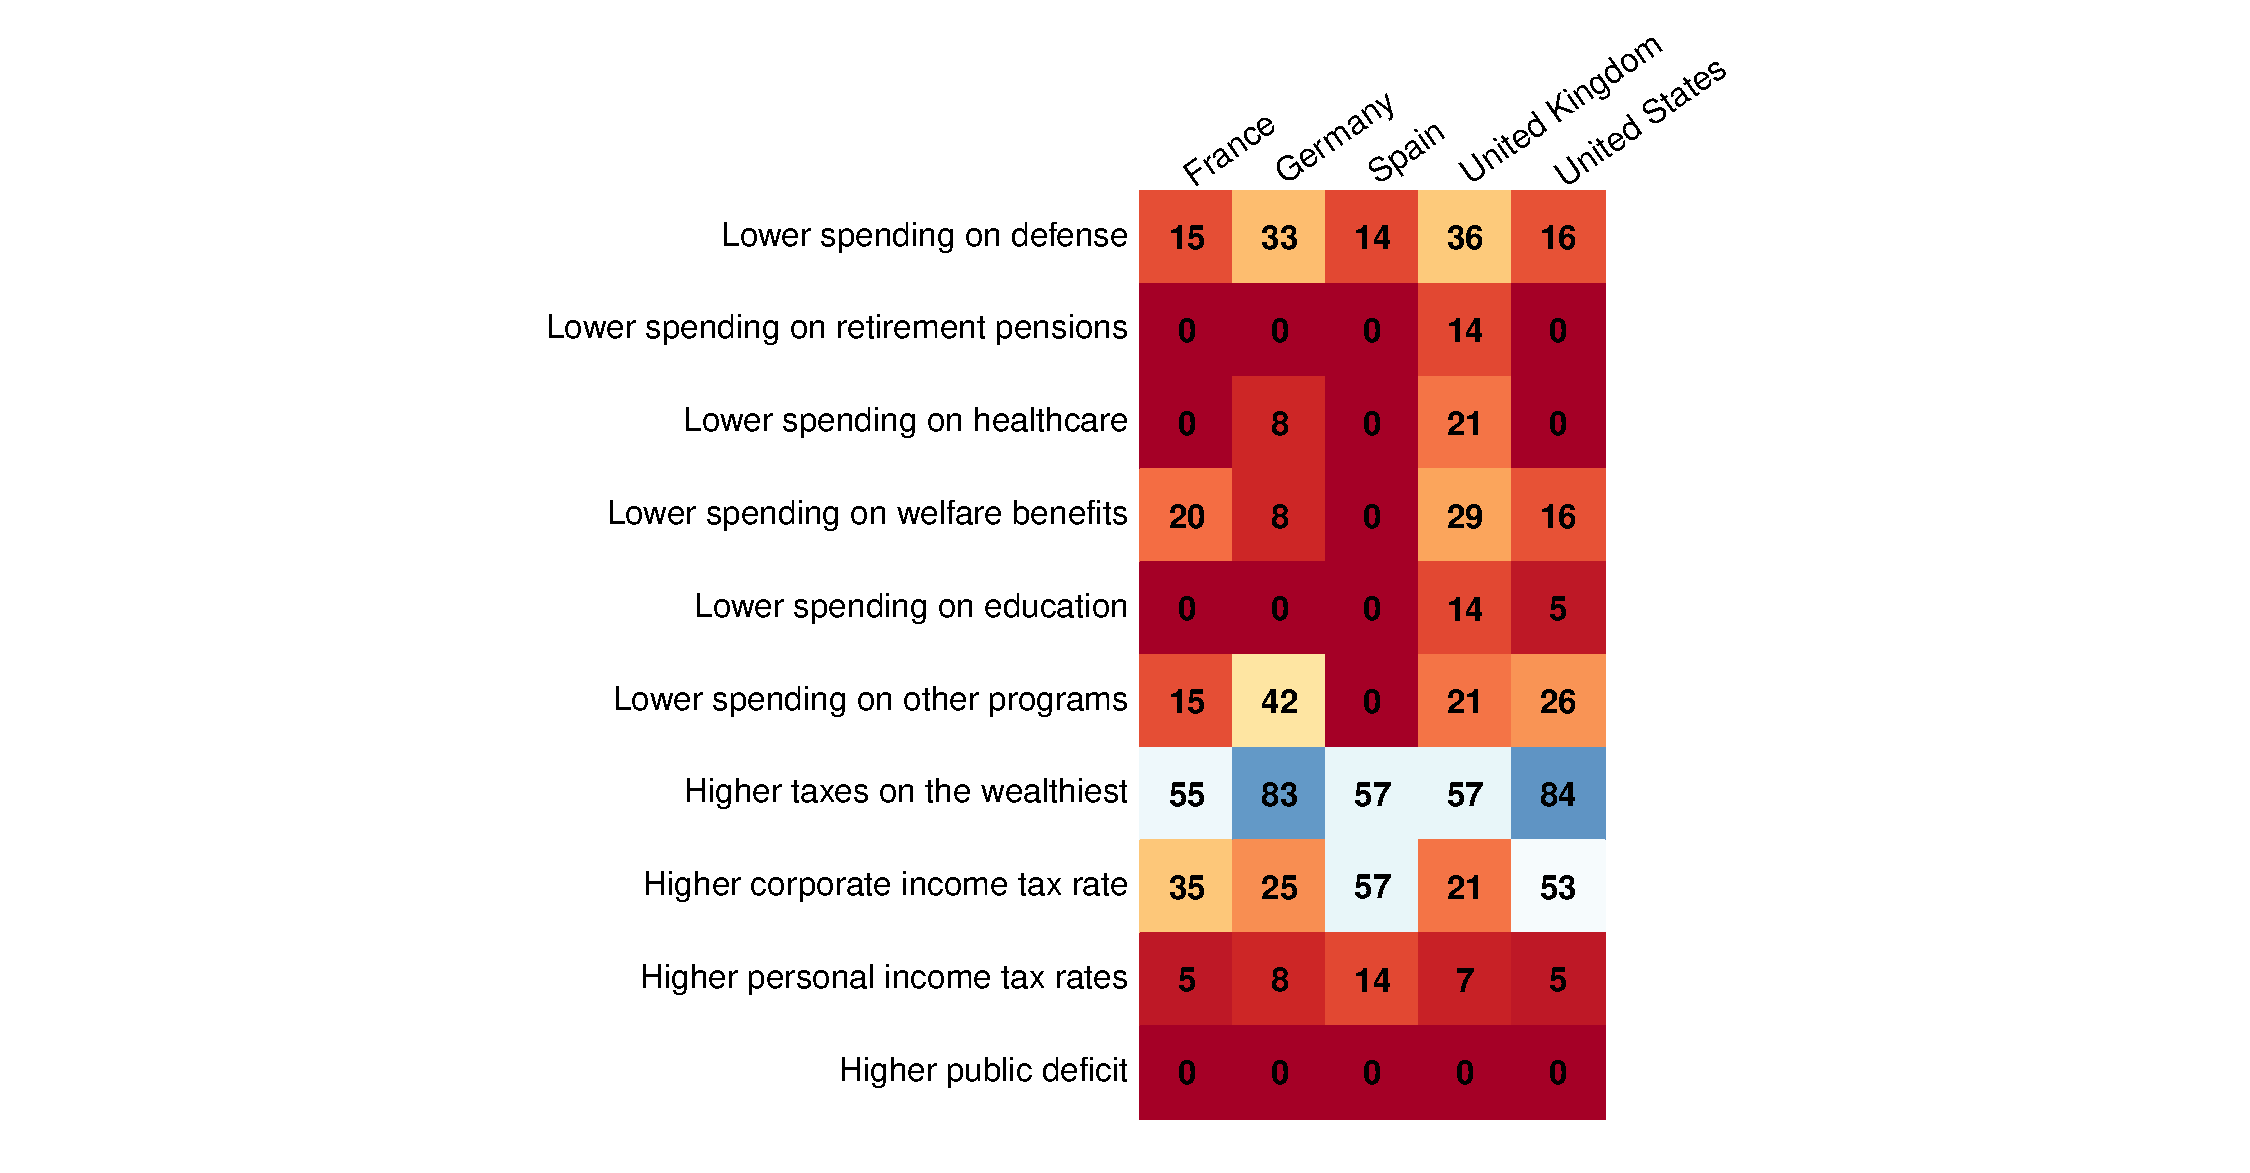
\includegraphics[width=.75\textwidth]{../figures/country_comparison/foreign_aid_raise_positive.pdf}} 
\end{figure}

\begin{figure}[h!]
    \caption[Preferences of spending following reduced foreign aid]{Preferences of spending following reduced foreign aid. [Asked iff preferred foreign aid is strictly lower than [Info: actual; No info: perceived] foreign aid] \\ ``How would you like to use the freed budget? (Multiple answers possible)'' (in percent) (Question \ref{q:foreign_aid_reduce_how})}\label{fig:foreign_aid_reduce_how}
    \makebox[\textwidth][c]{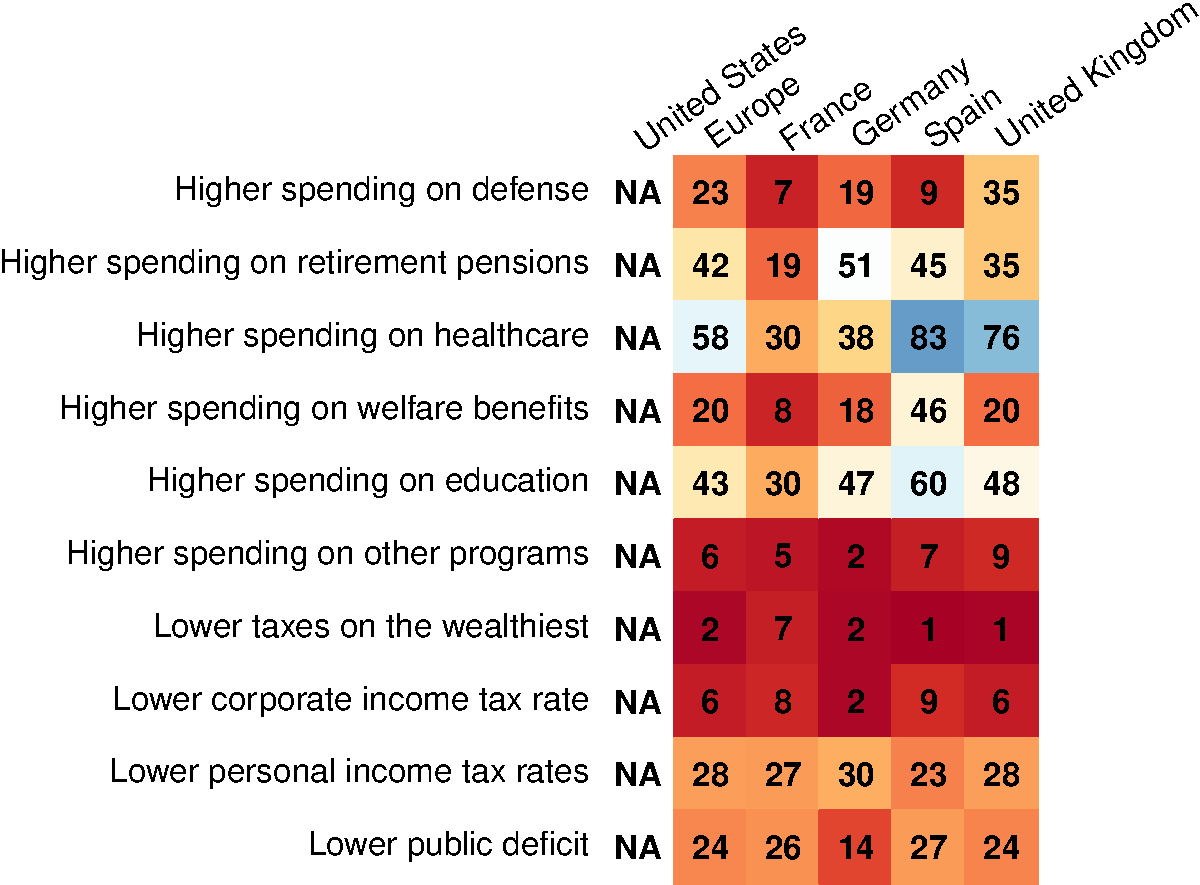
\includegraphics[width=.75\textwidth]{../figures/country_comparison/foreign_aid_reduce_positive.pdf}} 
\end{figure}

% \begin{figure}[h!]
%     \caption[Attitudes on the evolution of foreign aid]{Attitudes regarding the evolution of [own country] foreign aid. (Question \ref{q:foreign_aid_raise_support})}\label{fig:foreign_aid_raise_support}
%     \makebox[\textwidth][c]{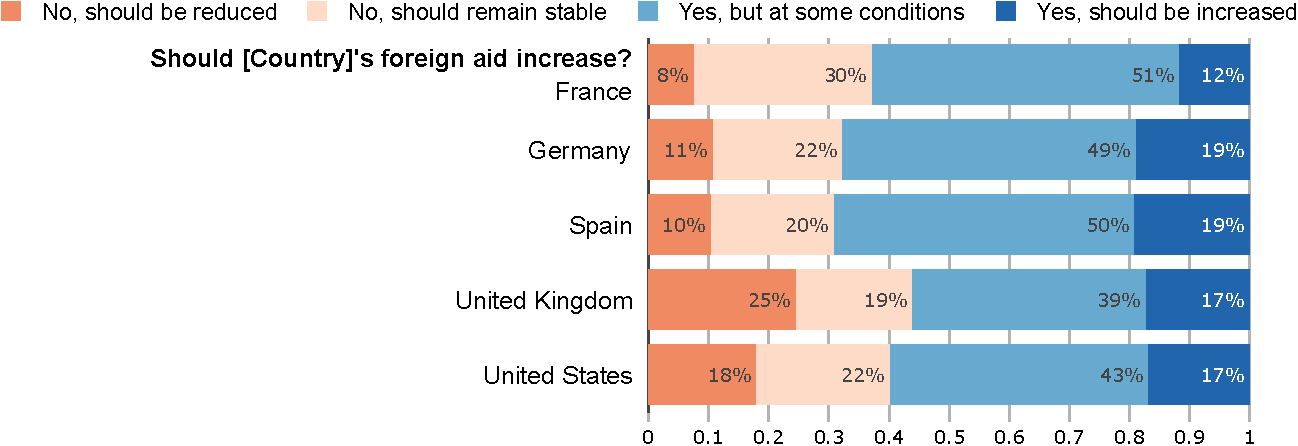
\includegraphics[width=\textwidth]{../figures/country_comparison/foreign_aid_raise_support.pdf}} 
% \end{figure}

% \begin{figure}[h!]
%     \caption[Conditions at which foreign aid should be increased]{Conditions at which foreign aid should be increased (in percent). [Asked to those who wish an increase of foreign aid at some conditions.] (Question \ref{q:foreign_aid_condition})}\label{fig:foreign_aid_condition}
%     \makebox[\textwidth][c]{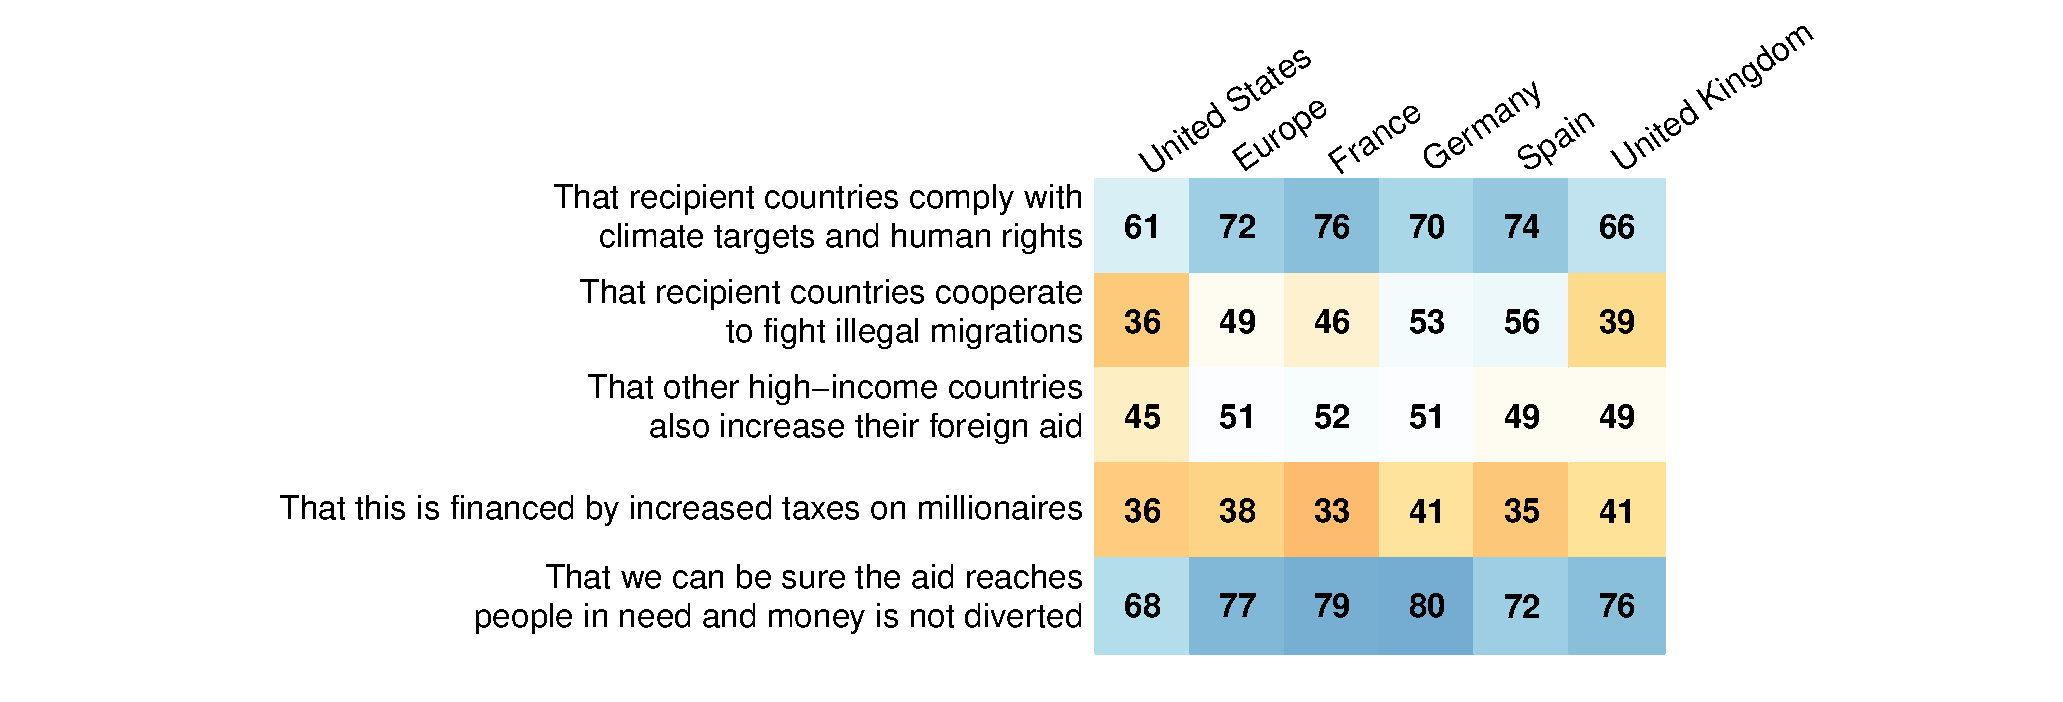
\includegraphics[width=\textwidth]{../figures/country_comparison/foreign_aid_condition_positive.pdf}} 
% \end{figure}

% \begin{figure}[h!]
%     \caption[Reasons why foreign aid should not be increased]{Reasons why foreign aid should not be increased (in percent). [Asked to those who wish a decrease or stability of foreign aid.] (Question \ref{q:foreign_aid_no})}\label{fig:foreign_aid_no}
%     \makebox[\textwidth][c]{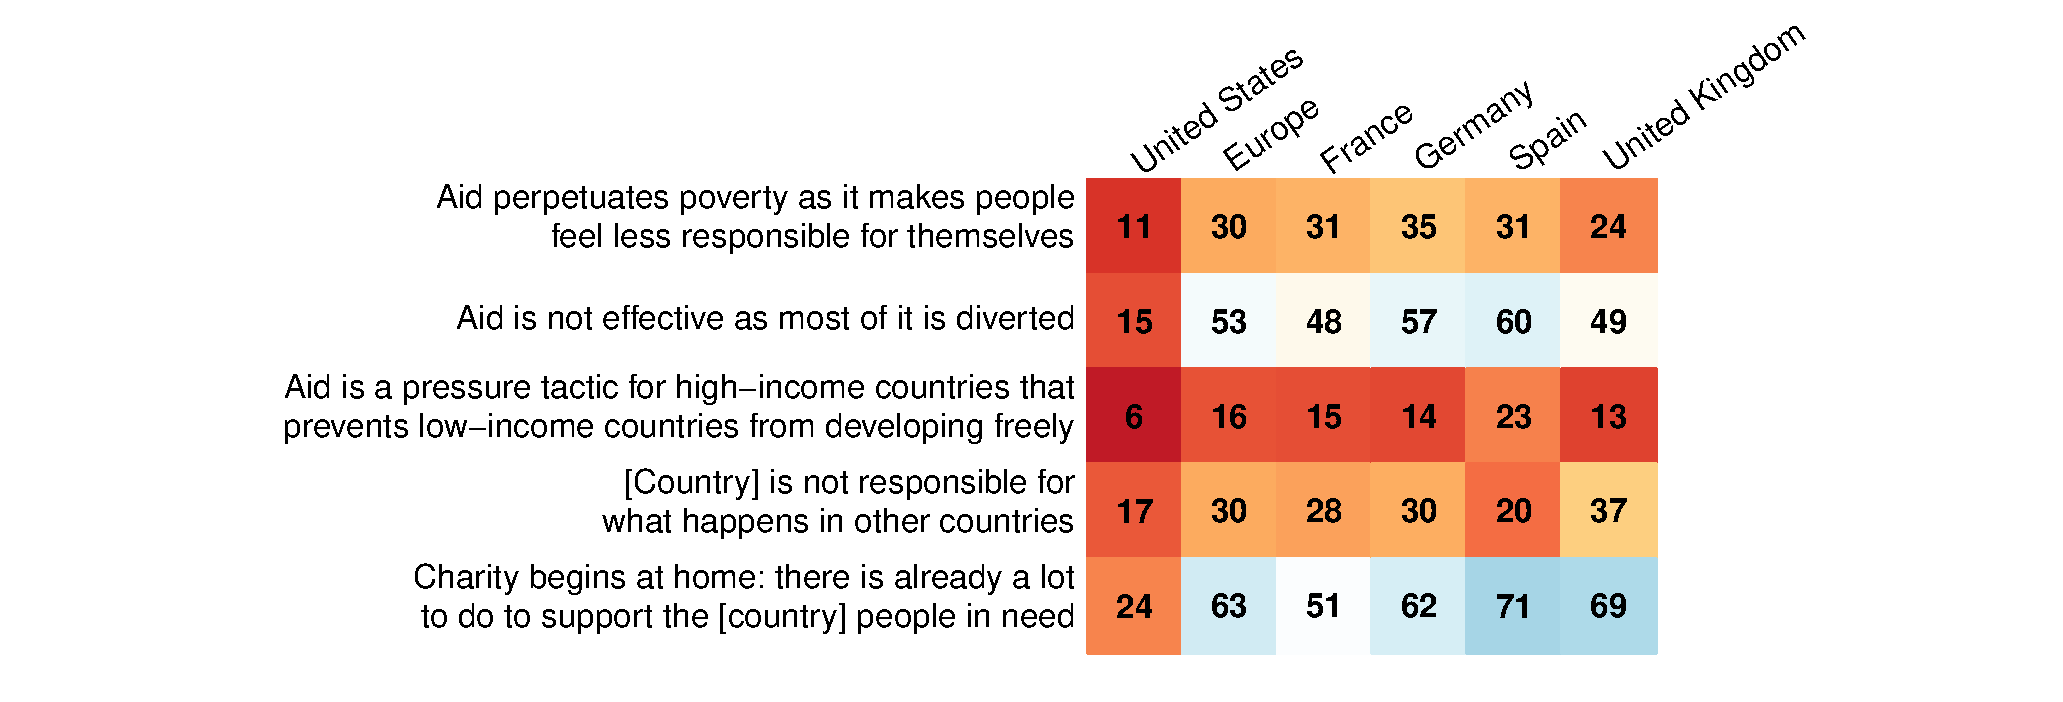
\includegraphics[width=\textwidth]{../figures/country_comparison/foreign_aid_no_positive.pdf}} 
% \end{figure}

% \begin{figure}[h!]
%     \caption[Willingness to sign a real-stake petition]{Willingness to sign real-stake petition for the Global Climate Scheme or National Redistribution. (Question \ref{q:petition})}\label{fig:petition}
%     \makebox[\textwidth][c]{
\includegraphics[width=.8\textwidth]{../figures/country_comparison/petition_only_positive.pdf}} 
% \end{figure}

\begin{figure}[h!]
    \caption[Willingness to sign a real-stake petition]{Willingness to sign real-stake petition for the Global Climate Scheme or National Redistribution, compared to stated support in corresponding subsamples (e.g. support for the GCS in the branch where the petition was about the GCS). (Question \ref{q:petition})}\label{fig:petition}
    \makebox[\textwidth][c]{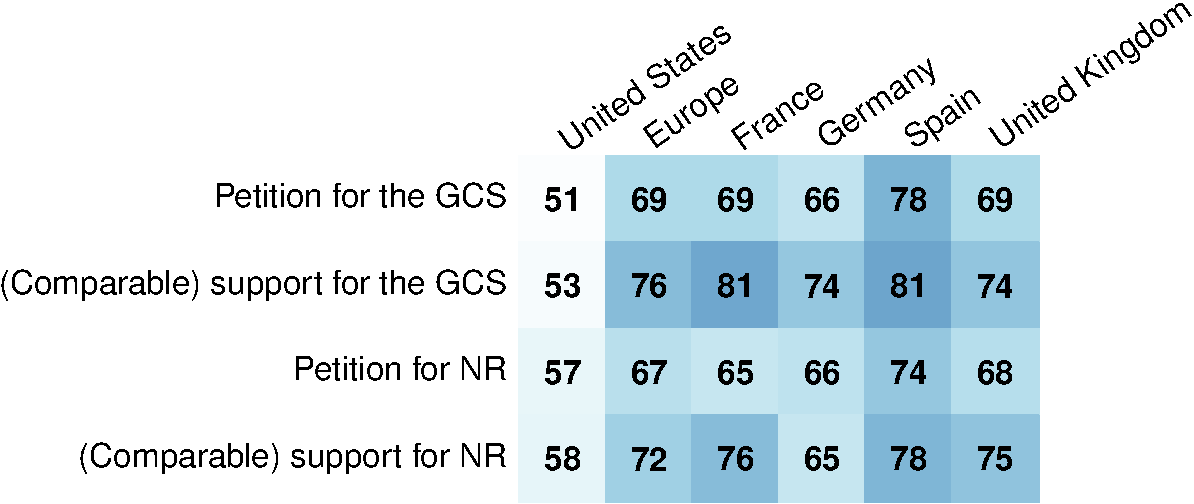
\includegraphics[width=.8\textwidth]{../figures/country_comparison/petition_comparable_positive.pdf}} 
\end{figure}

\begin{figure}[h!] % TODO? More details?
    \caption[Absolute support for various global policies]{Absolute support for various global policies (Percent of (\textit{somewhat} or \textit{strong}) support). (Questions \ref{q:climate_policies} and \ref{q:other_policies}. See Figure \ref{fig:support} for the relative support.)}\label{fig:support_likert_positive}
    \makebox[\textwidth][c]{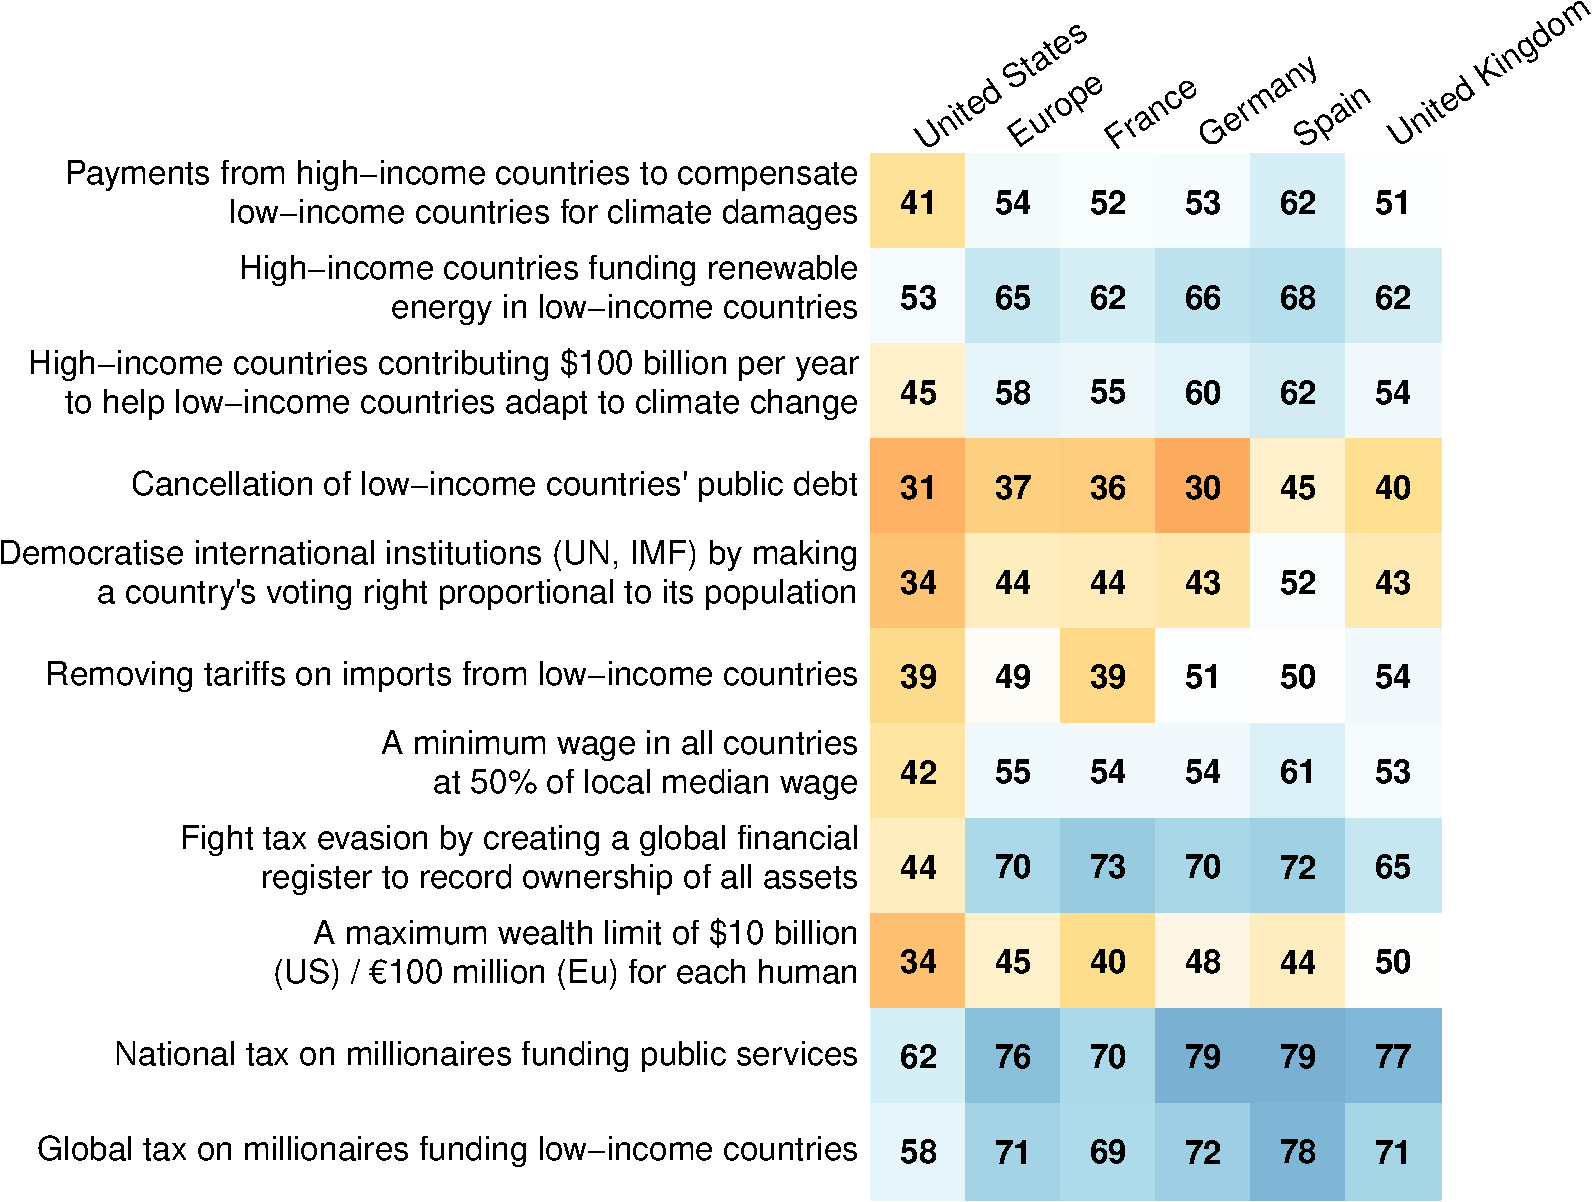
\includegraphics[width=\textwidth]{../figures/country_comparison/support_likert_positive.pdf}} 
\end{figure}

% \begin{figure}[h!]
%     \caption{label}\label{fig:climate_policies}
%     \makebox[\textwidth][c]{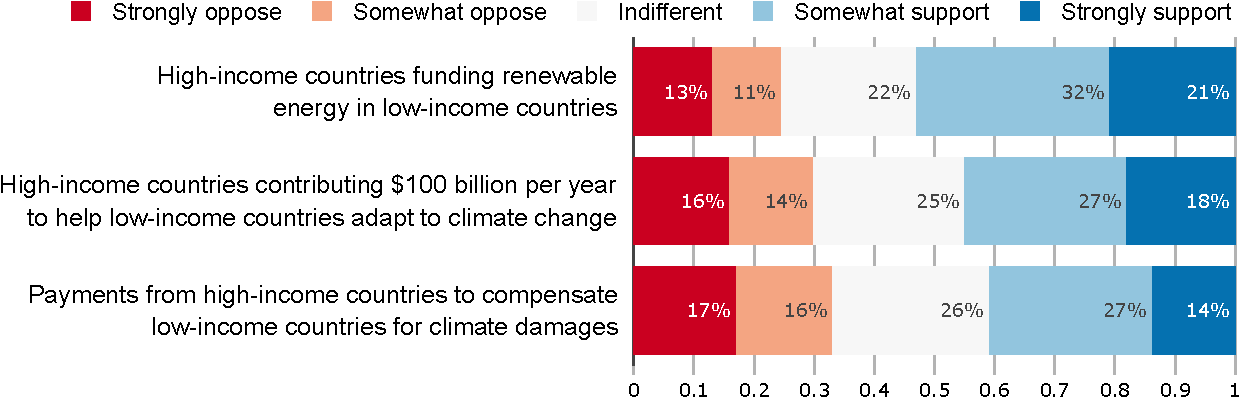
\includegraphics[width=\textwidth]{../figures/country_comparison/climate_policies.pdf}} 
% \end{figure}

% \begin{figure}[h!]
%     \caption{label}\label{fig:global_policies}
%     \makebox[\textwidth][c]{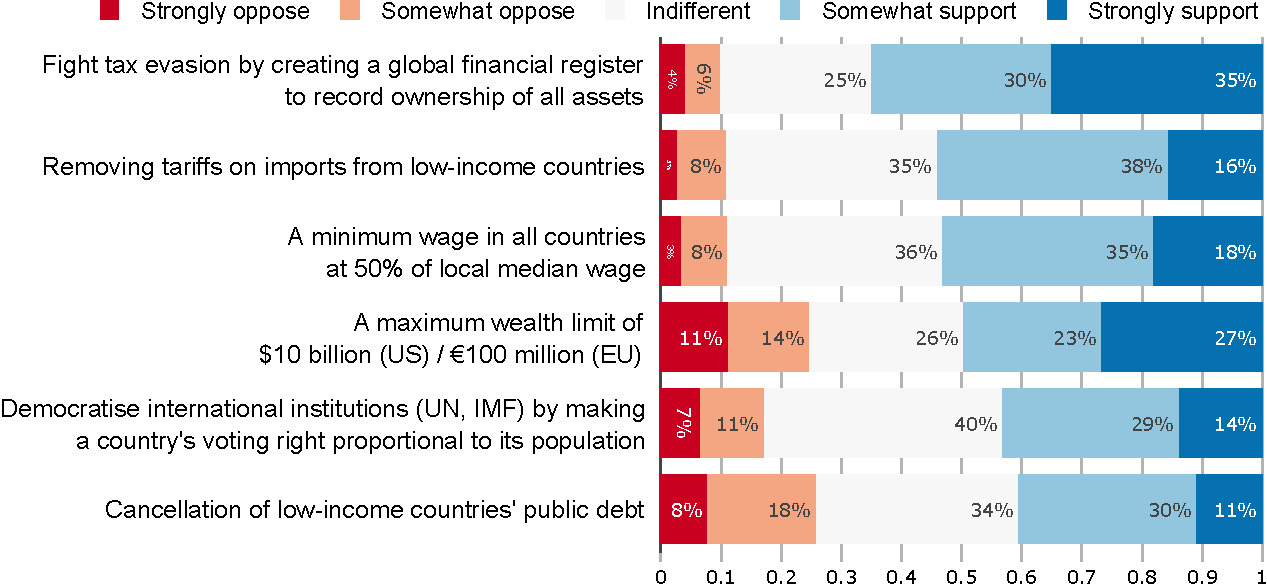
\includegraphics[width=\textwidth]{../figures/country_comparison/global_policies.pdf}} 
% \end{figure}

\begin{figure}[h!]
    \caption[Preferred approach for international climate negotiations]{Preferred approach of diplomats at international climate negotiations. \\ In international climate negotiations, would you prefer [U.S.] diplomats to defend [own country] interests or global justice? (Question \ref{q:negotiation})}\label{fig:negotiation}
    \makebox[\textwidth][c]{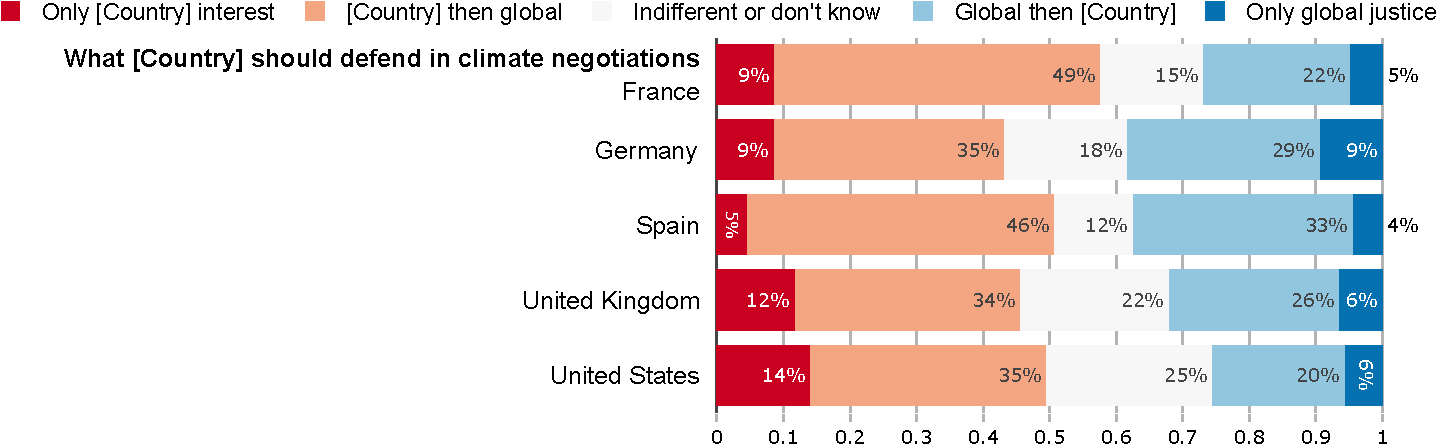
\includegraphics[width=\textwidth]{../figures/country_comparison/negotiation.pdf}} 
\end{figure}

\begin{figure}[h!]
    \caption[Importance of selected issues]{Percent of selected issues viewed as important.\\ ``To what extent do you think the following issues are a problem?'' (Question \ref{q:problem})}\label{fig:problem}
    \makebox[\textwidth][c]{
\includegraphics[width=.75\textwidth]{../figures/country_comparison/problem_positive.pdf}} 
\end{figure}

\begin{figure}[h!]
    \caption[Group defended when voting]{Group defended when voting. \\ ``What group do you defend when you vote?'' (Question \ref{q:group_defended})}\label{fig:group_defended}
    \makebox[\textwidth][c]{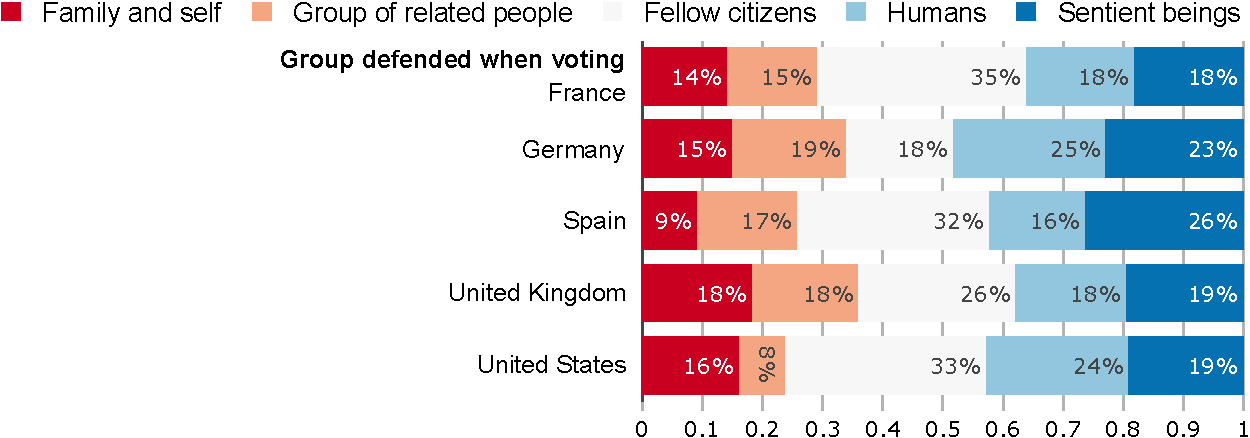
\includegraphics[width=\textwidth]{../figures/country_comparison/group_defended_agg2.pdf}} 
\end{figure}

% \begin{figure}[h!]
%     \caption{label}\label{fig:group_defended}
%     \makebox[\textwidth][c]{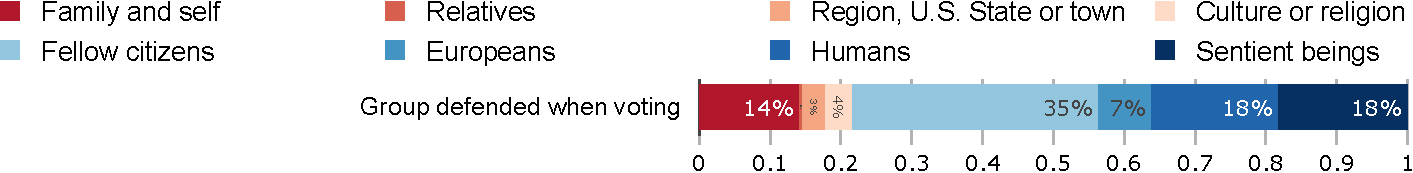
\includegraphics[width=\textwidth]{../figures/country_comparison/group_defended.pdf}} 
% \end{figure}

\begin{figure}[h!] 
    \caption[Mean prioritization of policies]{Mean prioritization of policies. \\Mean number of points allocated policies to express intensity of support (among six policies chosen at random). Blue color means that the policy has been awarded more points than the average policy. (Question \ref{q:points})}\label{fig:points}
    \makebox[\textwidth][c]{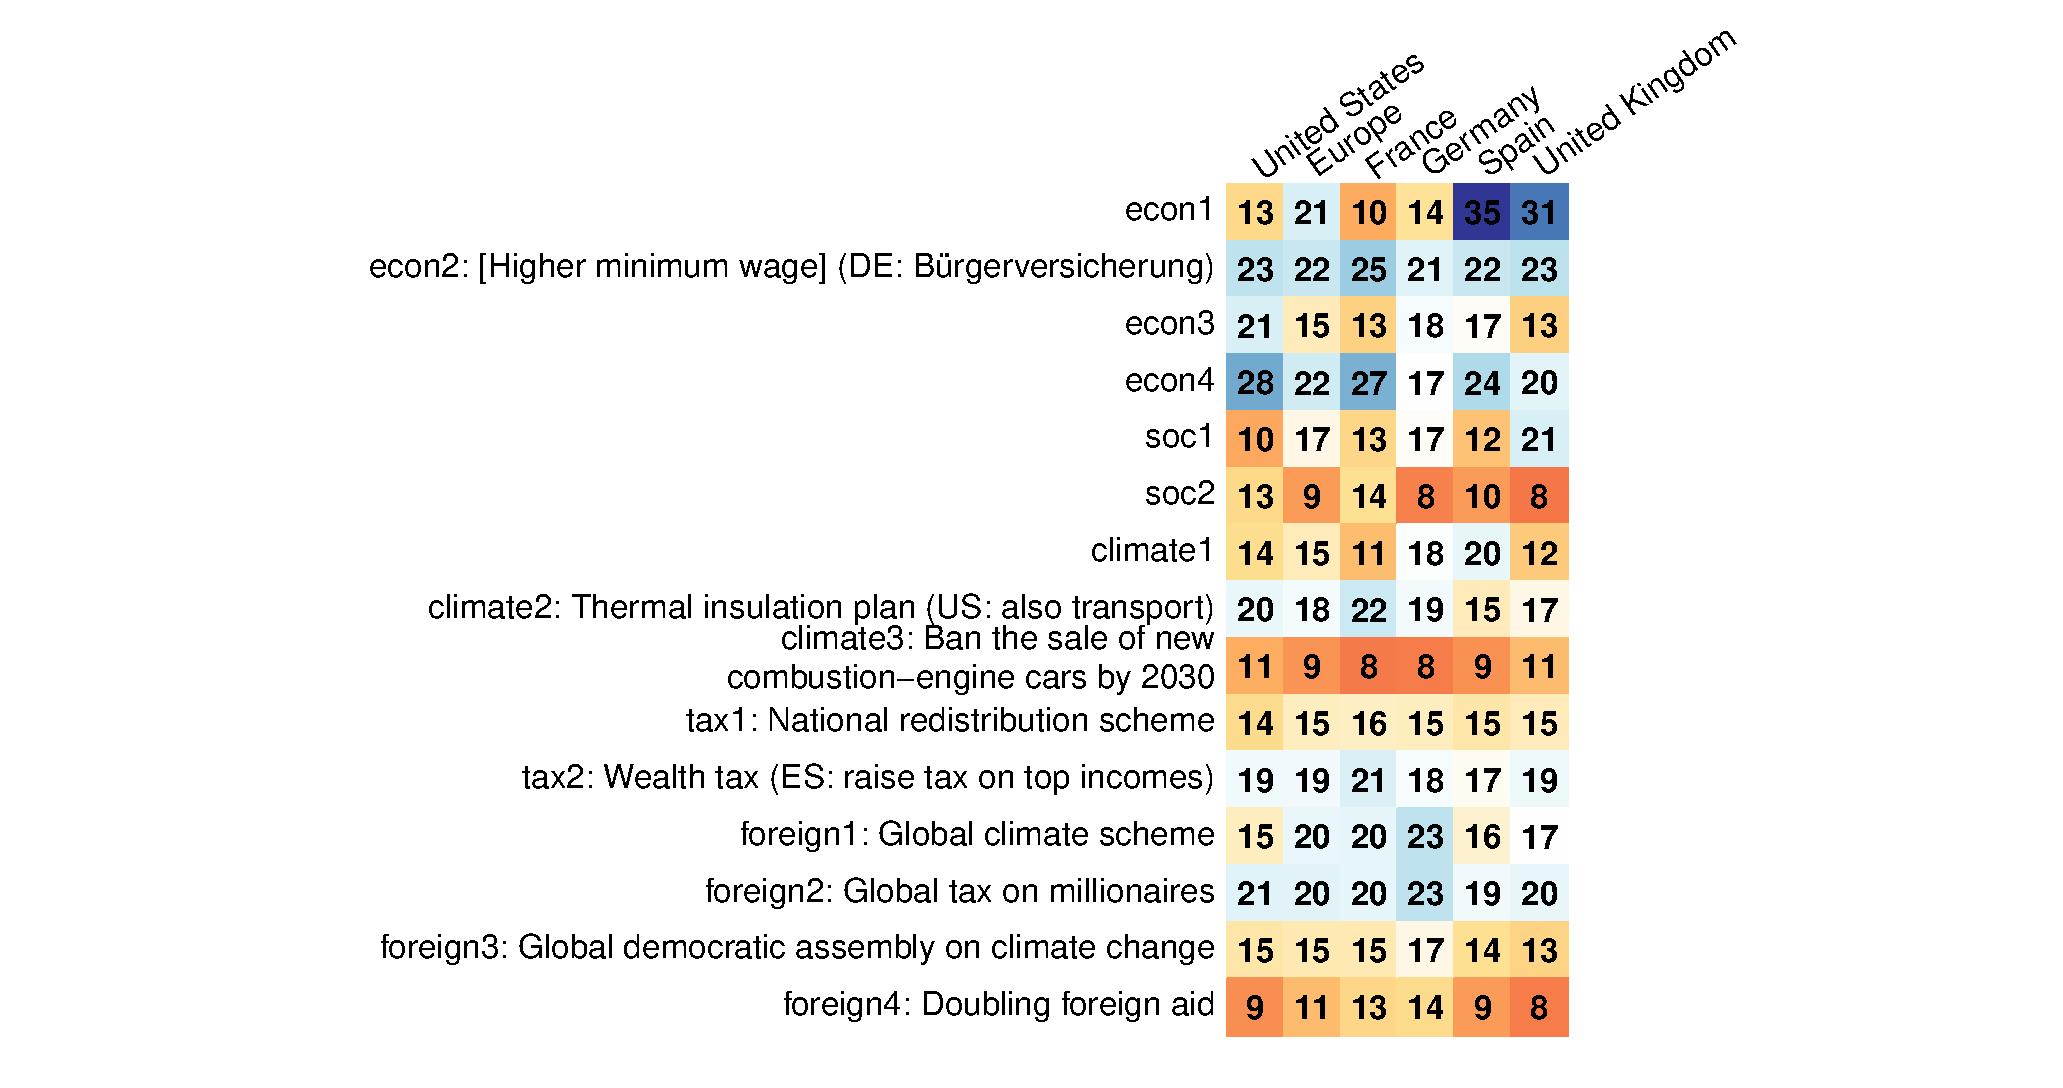
\includegraphics[width=\textwidth]{../figures/country_comparison/points_mean.pdf}} 
\end{figure}

\begin{figure}[h!] 
    \caption[Positive prioritization of policies]{Positive prioritization of policies. \\ Percent of people allocating a positive number of points to policies, expressing their support (among six policies chosen at random). (Question \ref{q:points})}\label{fig:points_positive}
    \makebox[\textwidth][c]{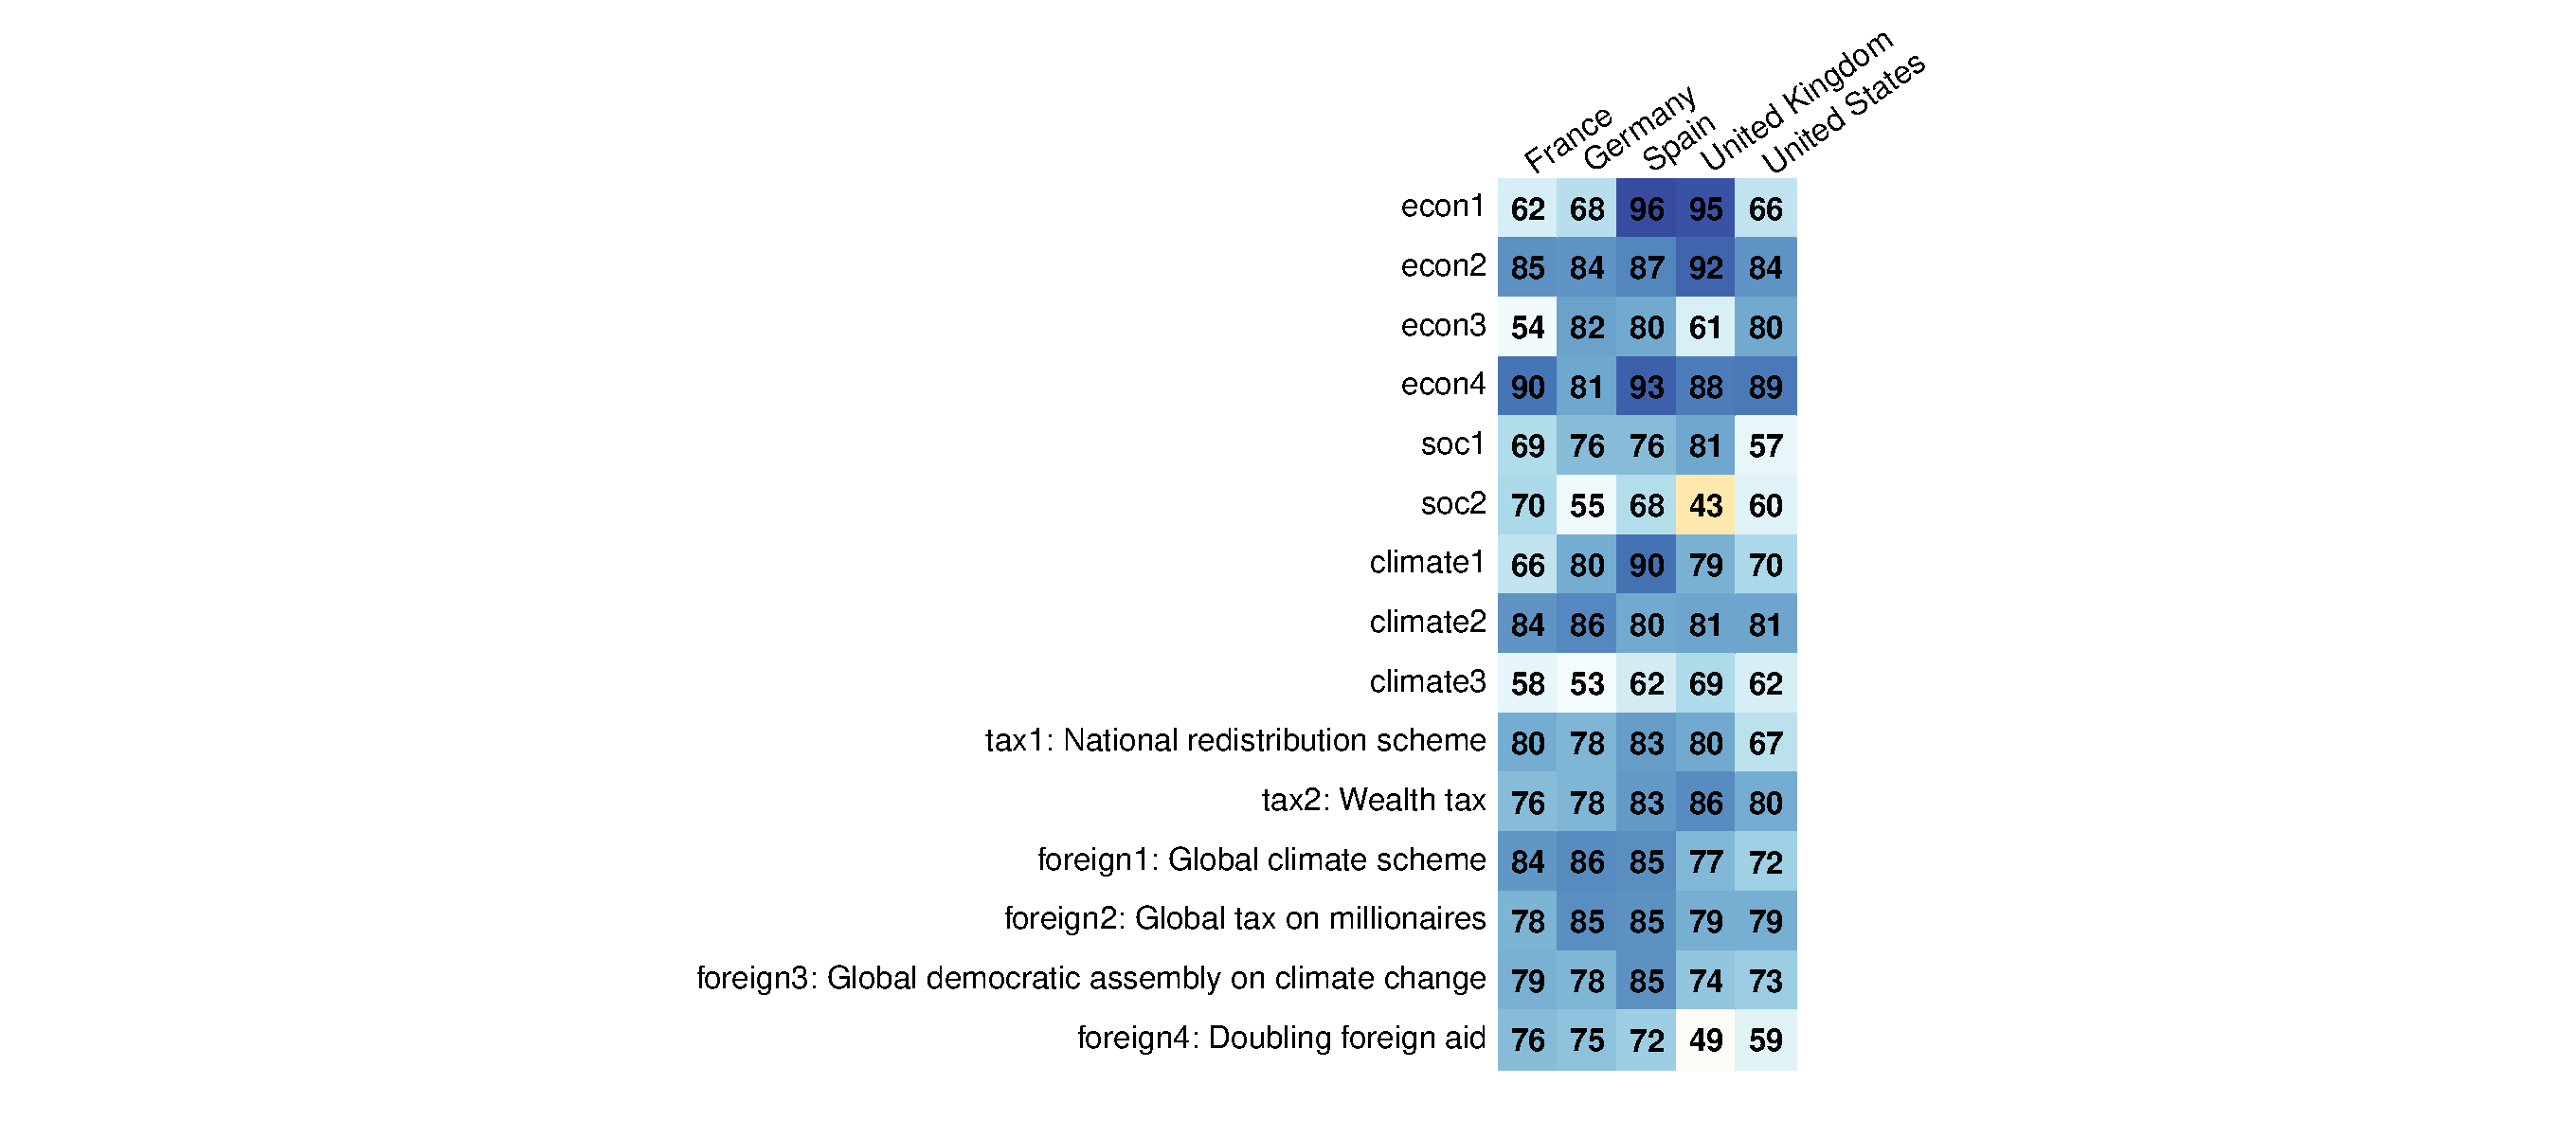
\includegraphics[width=\textwidth]{../figures/country_comparison/points_positive.pdf}} 
\end{figure}

\begin{figure}[h!]
    \caption[Charity donation]{Charity donation. \\ ``How much did you give to charities in 2022?'' (Question \ref{q:donation_charities})}\label{fig:donation_charities}
    \makebox[\textwidth][c]{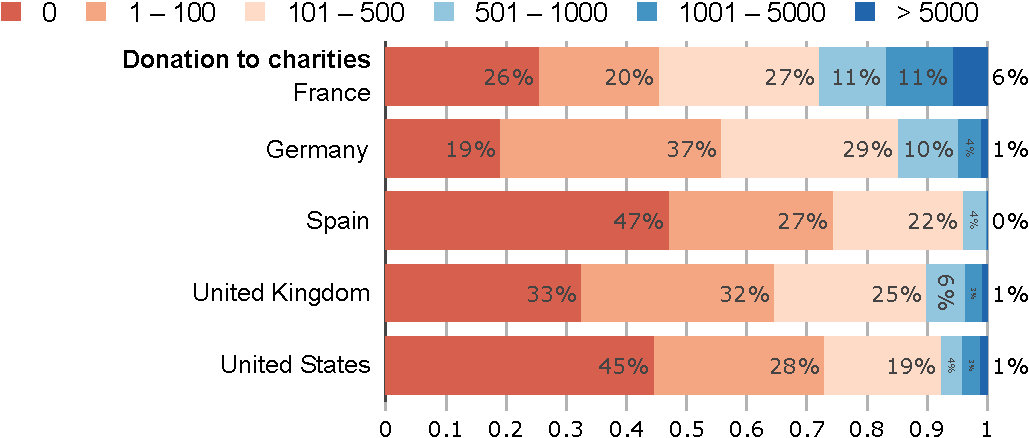
\includegraphics[width=.8\textwidth]{../figures/country_comparison/donation_charities.pdf}} 
\end{figure}

\begin{figure}[h!] 
    \caption[Interest in politics]{Interest in politics. \\ ``To what extent are you interested in politics?'' (Question \ref{q:interested_politics})}\label{fig:interested_politics}
    \makebox[\textwidth][c]{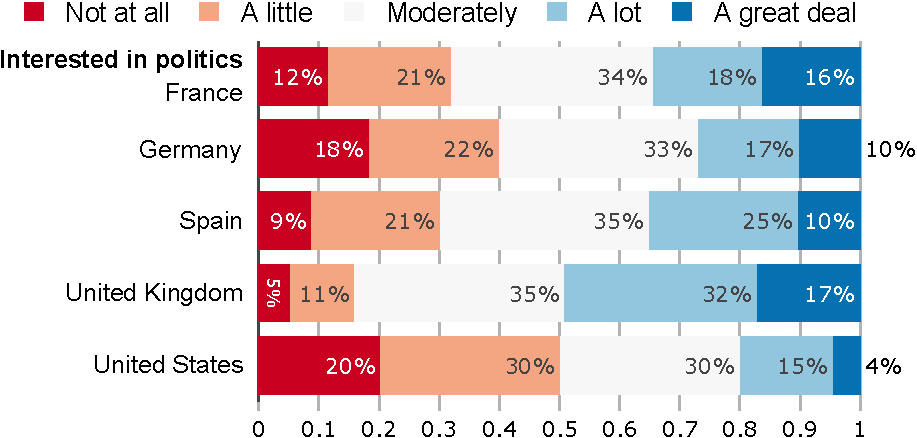
\includegraphics[width=.8\textwidth]{../figures/country_comparison/interested_politics.pdf}} 
\end{figure}

\begin{figure}[h!] 
    \caption[Desired involvement of government]{Desired involvement of government (from 1 to 5). (Question \ref{q:involvement_govt})}\label{fig:involvement_govt}
    \makebox[\textwidth][c]{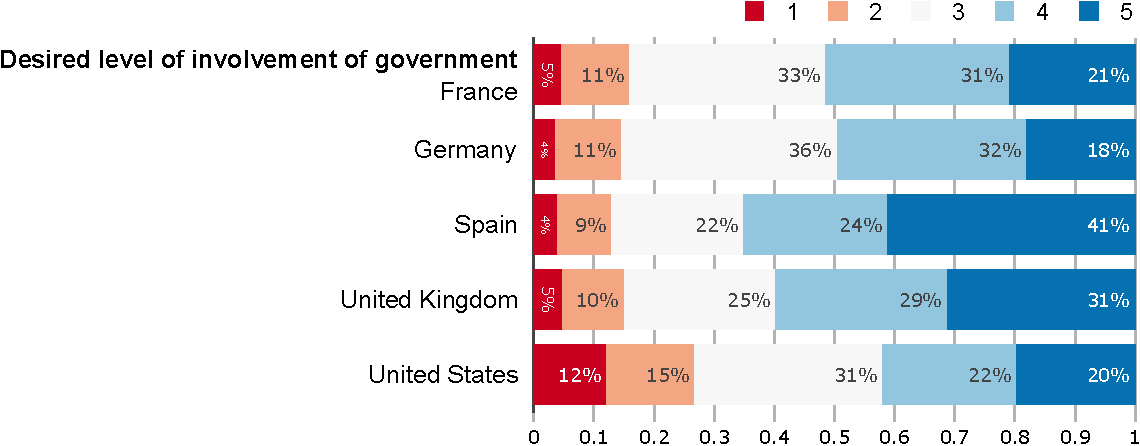
\includegraphics[width=.9\textwidth]{../figures/country_comparison/involvement_govt.pdf}} 
\end{figure}

\begin{figure}[h!] 
    \caption[Political leaning]{Political leaning on economics (from 1: Left to 5: Right). (Question \ref{q:left_right})}\label{fig:left_right}
    \makebox[\textwidth][c]{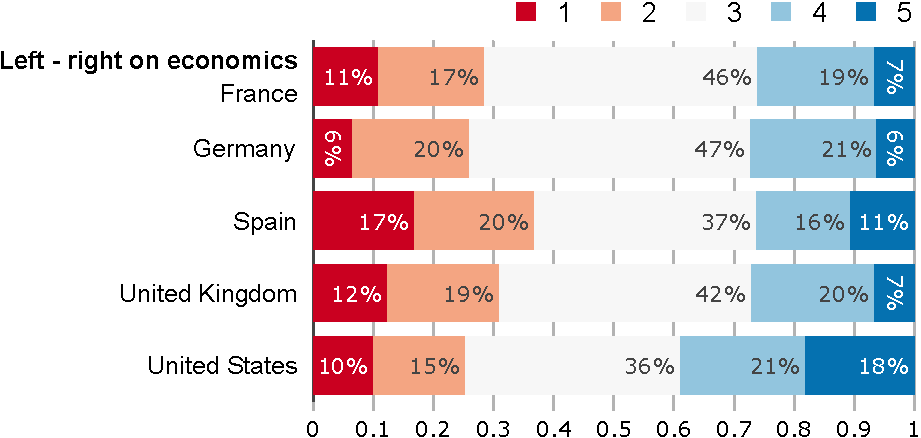
\includegraphics[width=.8\textwidth]{../figures/country_comparison/left_right.pdf}} 
\end{figure}

\begin{figure}[h!] 
    \caption[Voted in last election]{Voted in last election. (Question \ref{q:vote_participation})}\label{fig:vote_participation}
    \makebox[\textwidth][c]{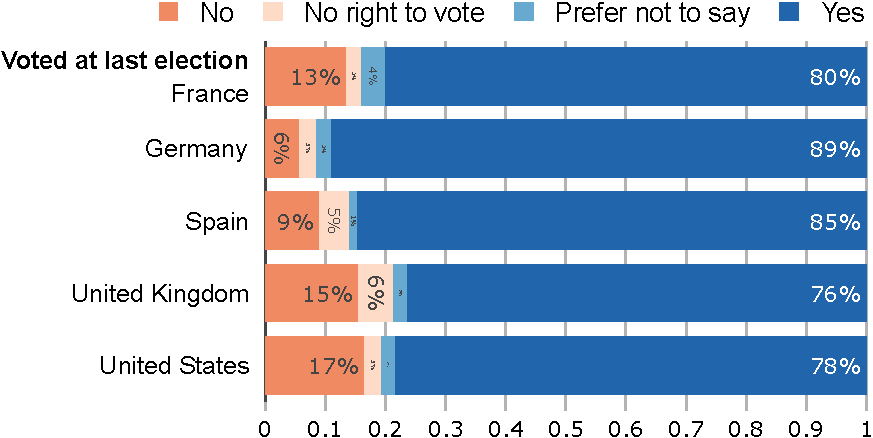
\includegraphics[width=.8\textwidth]{../figures/country_comparison/vote_participation.pdf}} 
\end{figure}

\begin{figure}[h!] 
    \caption[Vote in last election]{Vote in last election (aggregated). \textit{PNR} includes people who did not vote or prefer not to answer. (Question \ref{q:vote})}\label{fig:vote}
    \makebox[\textwidth][c]{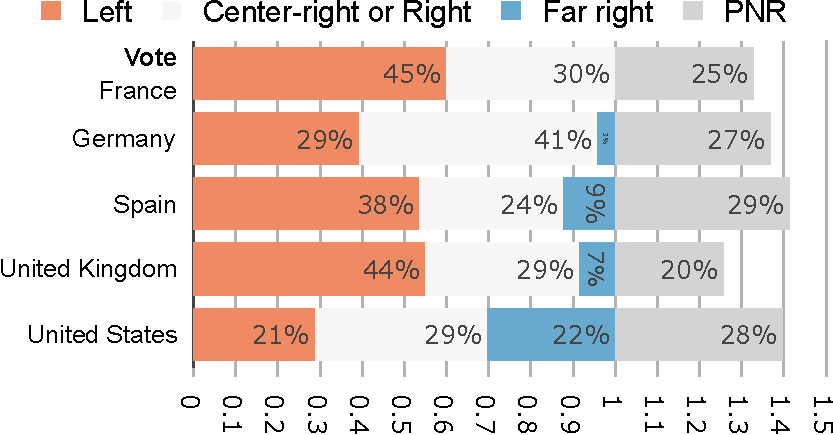
\includegraphics[width=.75\textwidth]{../figures/country_comparison/vote.pdf}} 
\end{figure}

\begin{figure}[h!] 
    \caption[Perception that survey was biased]{Perception that survey was biased. \\ ``Do you feel that this survey was politically biased?'' (Question \ref{q:survey_biased})}\label{fig:survey_biased}
    \makebox[\textwidth][c]{\includegraphics[width=.7\textwidth]{../figures/country_comparison/survey_biased.pdf}} 
\end{figure}

% \begin{columns}
% \begin{column}{.5\textwidth}
% \begin{multicols}{2}
    \begin{figure}[h!]
        \caption[Classification of open-ended field on extreme poverty]{Opinion on the fight against extreme poverty. \\ ``According to you, what should high-income countries do to fight extreme poverty in low-income countries?'' (Question \ref{q:poverty_field})}\label{fig:poverty_field}
    \begin{subfigure}{.34\textwidth}
        \caption{Elements found in the open-ended field on the question (manually recoded, in percent)}.
        \includegraphics[width=\textwidth]{../figures/country_comparison/poverty_field_positive.pdf}        
    \end{subfigure}
    \hspace{.02\textwidth}
    \begin{subfigure}{.64\textwidth}
        \caption{Keywords found in the open-ended field on the GCS (automatic search ignoring case, in percent).}
        \includegraphics[width=\textwidth]{../figures/country_comparison/poverty_field_contains_positive.pdf}    
    \end{subfigure}
    \end{figure}
% \end{column}
% \begin{column}{.5\textwidth}
    % \begin{figure}[h!]
    %     \caption[Topics of open-ended field on extreme poverty]{Opinion on the fight against extreme poverty. \\ ``According to you, what should high-income countries do to fight extreme poverty in low-income countries?'' \\ Keywords found in the open-ended field on the GCS (automatic search ignoring case, in percent). (Question \ref{q:poverty_field})}\label{fig:poverty_field_contains}
    %     \makebox[\textwidth][c]{\includegraphics[width=\columnwidth]{../figures/country_comparison/poverty_field_contains_positive.pdf}} 
    % \end{figure}
% \end{multicols}
% \end{column}
% \end{columns}


% \begin{figure}[h!] 
%     \caption[Interested to be interviewed]{Interested to be interviewed by a researcher for 30 min through videoconference. (Question \ref{q:interview})}\label{fig:interview}
%     \makebox[\textwidth][c]{\includegraphics[width=\textwidth]{../figures/country_comparison/interview.pdf}} 
% \end{figure}    

% \begin{figure}[h!]
%     \caption{label}\label{fig:share_policies_supported}
%     \makebox[\textwidth][c]{\includegraphics[width=\textwidth]{../figures/country_comparison/share_policies_supported.pdf}} 
% \end{figure} % TODO? uncomment?

% \begin{figure}[h!]
%     \caption{label}\label{fig:vars}
%     \makebox[\textwidth][c]{\includegraphics[width=\textwidth]{../figures/country_comparison/vars.pdf}} 
% \end{figure}

% In Denmark, France and the U.S., the questions with an asterisk were asked differently, asking ``To achieve a given reduction of greenhouse gas emissions globally, costly investments are needed. Ideally, how should countries bear the costs of fighting climate change?''. Instead of the equal right per capita, the item was ``Countries should pay in proportion to their current emissions'', historical responsibilities was worded as ``Countries should pay in proportion to their past emissions (from 1990 onwards)'', then there was an item ``The richest countries should pay it all'', and compensating vulnerable countries was worded as ``The richest countries should pay even more, to help vulnerable countries face adverse consequences: vulnerable countries would then receive money instead of paying''.

\clearpage 
\section{Questionnaire of the global survey (section on global policies)}\label{app:questionnaire_oecd}
%\subsection*{International burden-sharing}
\renewcommand{\theenumi}{\Alph{enumi}}
\begin{enumerate} \item \label{q:scale} At which level(s) do you think public policies to tackle climate change need to be put in place? (Multiple answers are possible) [\textit{Figures \ref{fig:oecd} and \ref{fig:oecd_absolute}}]
\\ \textit{Global; [Federal / European / ...]; [State / National]; Local}
\item Do you agree or disagree with the following statement: ``[country] should take measures to fight climate change.''% TODO! figure
	\\ \textit{Strongly disagree; Somewhat disagree; Neither agree nor disagree; Somewhat agree; Strongly agree}
\item How should [country] climate policies depend on what other countries do?% TODO! figure
 \begin{itemize}
\item If other countries do more, [country] should do...
\item If other countries do less, [country] should do...
\end{itemize}
\textit{Much less; Less; About the same; More; Much more}
\item ~[In all countries but the U.S., Denmark and France]  All countries have signed the Paris agreement that aims to contain global warming ``well below +2 \textdegree{}C\''. To limit global warming to this level, there is a maximum amount of greenhouse gases we can emit globally, called the carbon budget. Each country could aim to emit less than a share of the carbon budget. To respect the global carbon budget, countries that emit more than their national share would pay a fee to countries that emit less than their share. \\ 
Do you support such a policy? [\textit{Figures \ref{fig:oecd} and \ref{fig:oecd_absolute}}]
\\ \textit{Strongly oppose; Somewhat oppose; Neither support nor oppose; Somewhat support; Strongly support}
\item ~[In all countries but the U.S., Denmark and France] Suppose the above policy is in place. How should the carbon budget be divided among countries? [\textit{Figures \ref{fig:oecd} and \ref{fig:oecd_absolute}}]
\\ \textit{The emission share of a country should be proportional to its population, so that each human has an equal right to emit.; The emission share of a country should be proportional to its current emissions, so that those who already emit more have more rights to emit.; Countries that have emitted more over the past decades (from 1990 onwards) should receive a lower emission share, because they have already used some of their fair share.; Countries that will be hurt more by climate change should receive a higher emission share, to compensate them for the damages.}
\item \label{q:burden_sharing_asterisk} ~[In the U.S., Denmark, and France only] To achieve a given reduction of greenhouse gas emissions globally, costly investments are needed. % TODO! figure
Ideally, how should countries bear the costs of fighting climate change?
 \begin{itemize}
\item Countries should pay in proportion to their income
\item Countries should pay in proportion to their current emissions [Used as a substitute to the equal right per capita in Figure \ref{fig:oecd}]
\item Countries should pay in proportion to their past emissions (from 1990 onwards) [Used as a substitute to historical responsibilities in Figure \ref{fig:oecd}]
\item The richest countries should pay it all, so that the poorest countries do not have to pay anything
\item The richest countries should pay even more, to help vulnerable countries face adverse consequences: vulnerable countries would then receive money instead of paying [Used as a substitute to compensating vulnerable countries in Figures \ref{fig:oecd} and \ref{fig:oecd_absolute}]
\end{itemize} 
\textit{Strongly disagree; Somewhat disagree; Neither agree nor disagree; Somewhat agree; Strongly agree}
\item Do you support or oppose establishing a global democratic assembly whose role would be to draft international treaties against climate change? Each adult across the world would have one vote to elect members of the assembly. [\textit{Figures \ref{fig:oecd} and \ref{fig:oecd_absolute}}]
\\ \textit{Strongly oppose; Somewhat oppose; Neither support nor oppose; Somewhat support; Strongly support}
\item Imagine the following policy: a global tax on greenhouse gas emissions funding a global basic income. 
Such a policy would progressively raise the price of fossil fuels (for example, the price of gasoline would increase by [40 cents per gallon] in the first years). Higher prices would encourage people and companies to use less fossil fuels, reducing greenhouse gas emissions. Revenues from the tax would be used to finance a basic income of [\$30] per month to each human adult, thereby lifting the 700 million people who earn less than \$2/day out of extreme poverty. 
The average British person would lose a bit from this policy as they would face [\$130] per month in price increases, which is higher than the [\$30] they would receive.

Do you support or oppose such a policy?  [\textit{Figures \ref{fig:oecd} and \ref{fig:oecd_absolute}}]
\\ \textit{Strongly oppose; Somewhat oppose; Neither support nor oppose; Somewhat support; Strongly support}
\item \label{q:millionaire_tax} Do you support or oppose a tax on all millionaires around the world to finance low-income countries that comply with international standards regarding climate action? 
This would finance infrastructure and public services such as access to drinking water, healthcare, and education. [\textit{Figures \ref{fig:oecd} and \ref{fig:oecd_absolute}}]
\\ \textit{Strongly oppose; Somewhat oppose; Neither support nor oppose; Somewhat support; Strongly support}
\end{enumerate}

% \clearpage
% \section{Questionnaire of US1 %the first U.S. complementary 
% survey}\label{app:questionnaire_US1}

% \begin{figure}[h!]
%     \caption{US1 survey structure}\label{fig:flow_US1}
%     \makebox[\textwidth][c]{\includegraphics[width=\textwidth]{../questionnaire/survey_flow_US1.pdf}} 
% \end{figure}

\renewcommand{\theenumi}{\arabic{enumi}}
\clearpage
\section{Questionnaire of the complementary surveys}\label{app:questionnaire}
% /!\ Ctrl+H "\item ~[" / "\\ ["=> "\item ~[" / "\\ ~["
% TODO!? put in italic the "didascalies" in []
% TODO? give policies options here instead of referring to "this spreadsheet"
Below, we provide the generic questionnaire (based on the U.S. version), which roughly corresponds to the \textit{Eu} questionnaire as well as the combination of the \textit{US1} and \textit{US2} questionnaire. The main difference between Europe and the U.S. is that we split the \textit{US2} sample into four random branches to include some treatments before the Section \ref{subsec:questionnaire_GCS} on the GCS. Besides the control group, the treatments are: information regarding the support of Americans for the GCS and NR, an open-ended field, and a closed question on the pros and cons of the GCS. The pros and cons of the GCS are also asked in \textit{Eu} (likewise, either as an open-ended field or a question), but only in Section \ref{subsec:questionnaire_perceptions}, after the support. 

At each section or question, square brackets specify in which questionnaires it is present (\textit{US1}, \textit{US2} and/or \textit{Eu}) as well as country specificities. Figures \ref{fig:flow_Eu}-\ref{fig:flow_US2} display the structure of each questionnaire. Each treatment randomization is independent. Qualtrics and Word versions of the questionnaires in each language are available on our \href{https://github.com/bixiou/international_attitudes_toward_global_policies/tree/main/questionnaire}{public repository}, together with a spreadsheet that summarizes country specificities and our sources.

\begin{figure}[h!]
    \caption{\textit{Eu} survey structure}\label{fig:flow_Eu}
    \makebox[\textwidth][c]{\includegraphics[width=\textwidth]{../questionnaire/survey_flow_EU.pdf}} 
\end{figure}

\begin{figure}[h!]
    \caption{\textit{US1} survey structure}\label{fig:flow_US1}
    \makebox[\textwidth][c]{\includegraphics[width=\textwidth]{../questionnaire/survey_flow_US1.pdf}} 
\end{figure}

\begin{figure}[h!]
    \caption{\textit{US2} survey structure}\label{fig:flow_US2}
    \makebox[\textwidth][c]{\includegraphics[width=\textwidth]{../questionnaire/survey_flow_US2.pdf}} 
\end{figure}

\clearpage
\subsection*{[\textit{Eu}, \textit{US1}, \textit{US2}] Socio-demographic characteristics}
\begin{enumerate}
\item Welcome to this survey!\\
\\
This survey is \textbf{anonymous} and is conducted \textbf{for research} purposes on a representative sample of [1,000 British people].\\
 \\
It takes [\textit{US1}, \textit{US2}: 10 to 15 min; \textit{Eu}: around \textbf{20 min}] to complete.  \\
 \\
The survey contains lotteries and awards for those who get the correct answer to some understanding questions.\\
If you are attentive and lucky, \textbf{you can win up to }[\textit{US1}, \textit{Eu}: \textbf{\$350}; \textit{US2}: \textbf{\$150}] in points. (\href{https://uvafeb.eu.qualtrics.com/WRQualtricsControlPanel/File.php?F=F_cBZAXTgNktGZbee&download=1}{See terms and conditions}).    \\
Please answer every question carefully.  \\
 \\
\textbf{Do you agree to participate in the survey?}
\\ \textit{Yes; No}
\item What is your gender?
\\ \textit{Woman; Man; Other}
\item How old are you?
\\ \textit{Below 18; 18 to 20; 21 to 24; 25 to 29; 30 to 34; 35 to 39; 40 to 44; 45 to 49; 50 to 54; 55 to 59; 60 to 64; 65 to 69; 70 to 74; 75 to 79; 80 to 84; 85 to 89; 90 to 99; 100 or above}
\item ~[\textit{Eu}] In which country do you live?
\\ \textit{France; Germany; Spain; United Kingdom; Other}
\item What is your ZIP code? [UK: What is your Outcode (the left part of your postcode, e.g. if your postcode is N7 8H7, just enter N7)?]
\item \label{q:partner} Do you live with your partner (if you have one)?
\\ \textit{Yes; No}
\item How many people are in your household? The household includes: you, the members of your family who live with you, and your dependants. %This excludes flatmates.
\\ \textit{1; 2; 3; 4; 5 or more}
\item \label{q:children} [\textit{Eu}] How many children below 14 live with you?
\\ \textit{1; 2; 3; 4 or more}
\item ~[\textit{US1}, \textit{US2}] What race or ethnicity do you identify with? (Multiple answers are possible) 
\\ \textit{White; Black or African American; Hispanic; Asian; American Indian or Alaskan Native; Natice Hawaiian or Pacific Islander; Other: \{open field\}; Prefer not to say}
\item What is the [\textit{US1}, \textit{US2}: \textit{annual}; \textit{Eu}: \textit{monthly}] gross income of your household (before withholding tax)? This includes all income: wages, self-employment earnings, Social Security benefits, pensions, investment income, welfare payments, and income from other sources. % ~[quartiles thresholds are given for the U.S. ] 
\\ ~[\textit{US1}, \textit{US2}: Items based on household total income deciles and quartiles, namely: \textit{Less than \$20,000; between \$20,001 and \$35,000; between \$35,001 and \$42,000; between \$42,001 and \$50,000; between \$50,001 and \$65,000; between \$65,001 and \$82,000; between \$82,001 and \$103,000; between \$103,001 and \$130,000; between \$130,001 and \$145,000; between \$145,001 and \$165,000; between \$165,001 and \$250,000; More than \$250,000; I prefer not to answer}; \\ \textit{Eu}: custom thresholds, taking into account household composition Questions \ref{q:partner}-\ref{q:children}, and corresponding to the country's deciles and quartiles of standard of living, cf. the sheet ``Income'' in \href{https://github.com/bixiou/international_attitudes_toward_global_policies/raw/main/questionnaire/specificities.xlsx}{this spreadsheet}]
\item What is the highest level of education you have completed? 
\\ ~[\textit{Below upper secondary}, \textit{Upper secondary}, and \textit{Post secondary} are coded as the first two, middle three, and last three items, respectively. \\ \textit{US1}, \textit{US2}: \textit{Primary school or less; Eigth grade; Some high school; Regular high school diploma/GED or alternative credential; Some college, no degree; 2-year college degree or associates degree (for example: AA, AS); Bachelor's degree (for example: BA, BS); Master’s degree or above (MA, MS, MEng, MEd, MSW, MBA, MD, DDS, DVM, LLB, JD, PhD); } \\FR: \textit{École primaire / Aucun; Brevet; CAP ou BEP; Baccalauréat professionnel ou technologique; Baccalauréat général; Bac +2 (BTS, DUT, DEUG…); Bac +3 (licence…); Bac +5 ou plus (master, école d'ingénieur ou de commerce, doctorat, médecine, maîtrise, DEA, DESS...)} \\DE: \textit{Keine abgeschlossene Schulbildung / Grundschule; Untere Sekundarstufe (z.B. Haupt- oder Realschulabschluss); Erstausbildung; Beruflicher Abschluss / Ausbildung; Abitur; Zweitausbildung; Bachelor oder Fachhochschulabschluss; Master-Abschluss oder höher} \\ ES: \textit{Educación primaria / No he completado la enseñanza básica; Educación secundaria obligatoria (ESO); Formación profesional básica (FP); Formación profesional de grado medio; Bachillerato; Formación profesional de grado superior; Grado universitario; Máster/doctorado}\\ UK: \textit{Primary education or less; Some secondary school; GSCE; Vocational Upper secondary (Level 3 award, level 3 certificate, level 3 diploma, advanced apprenticeship, etc.); High school degree (A level); Higher vocational education (Level 4+ award, level 4+ certificate, level 4+ diploma, higher apprenticeship, etc.); Bachelor's Degree (BA, BSc, BEng, etc.); Postgraduate diploma or certificate, Master's Degree (MSc, MA, MBA, etc.) or Ph.D.}]
\item What is your employment status? \label{item:employment}
\\ \textit{Full-time employed; Part-time employed; Self-employed; Student; Retired; Unemployed (searching for a job); Inactive (not searching for a job)}
\item Are you a homeowner or a tenant? (Multiple answers are possible) 
\\ \textit{Tenant; Owner; Landlord renting out property; Hosted free of charge}
\item ~[If lives with partner: What is the estimated value of your household's assets (in U.S. dollars)?  \\
 If does not live with partner: What is the estimated value of your assets (in U.S. dollars)?]
   \\
Include here all your possessions (home, car, savings, etc.) net of debt. For example, if you own a house worth [\$]300,000 and you have [\$]100,000 left to repay on your mortgage, your assets are [\$]200,000.  \\
  \\
I estimate my [If lives with partner: household's] assets net of debt to be:  \\% ~[Quintiles thresholds are given for the U.S. ]
% \\ ~[Items based on wealth quintiles. US1, \textit{US2}: \textit{Less than \$0 (I have a net debt); Close to \$0; Between \$4,000 and \$120,000; Between \$120,000 and \$380,000; More than \$380,000}; For Eu, the thresholds are: FR: \euro{}10/100/300/600k; DE: \euro{}0/70/260/560k; ES: \euro{}0/100/200/400k; UK: £6/90/230/530k] 
\\ ~[Items based on the following individual wealth quintiles, doubled if lives with partner. \textit{US1}, \textit{US2}: \textit{Less than \$0 (I have a net debt); Close to \$0; Between \$4,000 and \$60,000; Between \$60,000 and \$190,000; More than \$190,000}; For \textit{Eu}, the thresholds are: FR: \euro{}5/50/150/300k; DE: \euro{}0/35/130/280k; ES: \euro{}0/50/100/200k; UK: £3/45/115/270k] 
% \item ~[Asked if does not live with partner] What is the estimated value of your assets (in U.S. dollars)?   \\
%    \\
% Include here all your possessions (home, car, savings, etc.) net of debt. For example, if you own a house worth [\$]300,000 and you have [\$]100,000 left to repay on your mortgage, your assets are [\$]200,000.  \\
%   \\
%   I estimate my assets net of debt to be: \\% ~[Quintiles thresholds are given for the U.S. ]
% \\ ~[Items based on wealth quintiles. US1, \textit{US2}: \textit{Less than \$0 (I have a net debt); Close to \$0; Between \$4,000 and \$60,000; Between \$60,000 and \$190,000; More than \$190,000}; For Eu, the thresholds are: FR: \euro{}5/50/150/300k; DE: \euro{}0/35/130/280k; ES: \euro{}0/50/100/200k; UK: £3/45/115/270k] 
\item \label{q:political_affiliation} ~[\textit{US1}, \textit{US2} (where it is instead asked toward the end, after the vote question)] What do you consider to be your political affiliation, as of today?
\\ \textit{Republican; Democrat; Independent; Other; Non-Affiliated}
\end{enumerate}

\subsection*{[\textit{Eu}, \textit{US1}, \textit{US2}] Global climate scheme}\label{subsec:questionnaire_GCS}
\begin{enumerate}[resume] \item[] In the following, we describe two policies, on which we will survey your opinion. To check that you have attentively read the descriptions,~\textbf{we will ask some understanding questions afterwards: those who get correct answers can win up to \$150}. \\
\textbf{\underbar{Global climate scheme:}}~ At the Paris agreement in 2015, all countries have agreed to contain global warming ``well below +2 $\mathrm{{}^\circ}$C''. To limit global warming to this level,~\textbf{there is a maximum amount of greenhouse gases we can emit globally}.\\
To meet the climate target, a limited number of permits to emit greenhouse gases can be created globally. Polluting firms would be required to buy permits to cover their emissions. Such a policy would~\textbf{make fossil fuel companies pay}~for their emissions and progressively raise the price of fossil fuels.~\textbf{Higher prices would encourage people and companies to use less fossil fuels, reducing greenhouse gas emissions.}\\
In accordance with the principle that each human has an equal right to pollute, the revenues generated by the sale of permits could finance a global basic income.~\textbf{Each adult in the world would receive } [\textit{US1}, \textit{US2}: \textbf{\$30/month}; UK: \textbf{\$30 (that is £25) per month}; FR, DE, ES:  \textbf{\euro{}30/month}], thereby lifting out of extreme poverty the 700 million people who earn less than \$2/day.\\
\textbf{The typical }[\textbf{American}]\textbf{ would lose out financially }[\textit{US1}, \textit{US2}: \textbf{\$85}, FR: \textbf{\euro{}10}, DE: \textbf{\euro{}25}, ES: \textbf{\euro{}5}, UK: \textbf{£20}]\textbf{ per month}~(as he or she would face [\$115] per month in price increases, which is higher than the [\$30] they would receive). 
\\The policy could be put in place as soon as countries totaling more than 60\% of global emissions agree on it. Countries that would refuse to take part in the policy could face sanctions (like tariffs) from the rest of the World and would be excluded from the basic income. \hfill (Back~to~Section~\ref{subsubsec:global_support})
\item \label{q:understood_gcs} Who would win or lose financially in the Global climate scheme? [\textit{Figure \ref{fig:understood_each}}] \\
\\
Three respondents with the expected answer will get [\$]50 in points.
\\ \textit{Typical [Americans] would win and the 700 million poorest humans would win.; \\Typical [Americans] would win and the 700 million poorest humans would lose.; \\Typical [Americans] would lose and the 700 million poorest humans would win.; \\Typical [Americans] would lose and the 700 million poorest humans would lose.}
\item[[new page\!\!\!]] For your information, the expected answer was \textit{Typical [Americans] would lose and the 700 million poorest humans would win} from the Global climate scheme. Now, here is the second policy: \\ 
\\
\textbf{\underbar{National redistribution scheme:}}\\ This policy would \textbf{increase taxes on the top} [\textit{US1}, \textit{US2}: \textbf{5\%}; 
\textit{Eu}: \textbf{1\%}] and provide cash transfers to all adults. More precisely, \textbf{each }[\textbf{American}]\textbf{ adult would receive }[\textbf{\$85}]\textbf{ per month} (that is [\$1,000] per year). 
This would be financed by an increase of the federal income tax on household income in excess of [\textit{US1}, \textit{US2}: \$315,000 per year; FR: \euro{}15,000 per month; DE: \euro{}20,000 per month; ES: \euro{}10,000 per month; UK: £15,000 per month], leaving taxes unchanged for income below [\$315,000]. [\textit{US1}, \textit{US2}: \underbar{See more details}.]
\footnote{8\% of U.S. respondents click. They then see the following text, based on \href{https://taxjusticenow.org/\#makeYourOwnTaxPlan}{taxjusticenow.org} by \citet{saez_triumph_2019}: \textit{The marginal income taxe rates would evolve as follows:\\Below \$315,000: unchanged \\ ~\$315,000 - \$400,000: current rate 32\% =$>$ new rate 41\% \\ ~\$400,000 - \$600,000: 35\% =$>$ 50\% \\ ~\$600,000 - \$2.5 million: 37\% =$>$ 60\% \\ ~\$2.5 - \$5 million: 37\% =$>$ 65\% \\ Above \$5 million: 37\% =$>$ 70\%}}
\item \label{q:understood_nr} Who would win or lose financially in the National redistribution? [\textit{Figure \ref{fig:understood_each}}] ~\\
\\
Three respondents with the expected answer will get [\$]50 in points.
\\ \textit{Typical [Americans] would win and the richest [Americans] would win.; Typical [Americans] would win and the richest [Americans] would lose.; Typical [Americans] would lose and the richest [Americans] would win.; Typical [Americans] would lose and the richest [Americans] would lose.}
\item[[new page\!\!\!]] For your information, the expected answer was \textit{Typical [Americans] would win and the richest [Americans] would lose} from the National redistribution scheme. \\ 
\\
To help you with the next question, here is a reminder of the policies:\\
\\
\textbf{\underbar{Global Climate scheme:}}\\ 
To limit global warming and reach the international climate objective, the Global climate scheme would \textbf{impose a maximum amount of greenhouse gases we can emit globally}.\\
It would \textbf{make polluters pay} for their emissions, which in turn would increase fossil fuel prices and discourage polluting activities.\\
The revenues would finance a \textbf{global basic income} of [\$30] per month for all humans, lifting out of extreme poverty the poorest billion people.\\
Considering the basic income and the fuel price increases, \textbf{the typical }[\textbf{American}]\textbf{ would lose out financially }[\textbf{\$85}]\textbf{ per month}.\\
\\
\textbf{\underbar{National redistribution scheme:}} \\This policy would \textbf{increase taxes on the top }[\textbf{5\%}] and provide cash transfers to all adults. More precisely, \textbf{each }[\textbf{American}]\textbf{ would receive }[\textbf{\$85}]\textbf{ per month}. This would be financed by an increase of the federal income tax on household income in excess of [\$315,000 per year], leaving taxes unchanged for income below [\$315,000 per year].
\item \label{q:understood_both} If both the Global climate scheme and the National redistribution scheme are implemented, how would a typical [American] be financially affected? [\textit{Figure \ref{fig:understood_each}}] \\
Three respondents with the expected answer will get [\$]50 in points.
\\ \textit{A typical [American] would lose out financially.; A typical [American] would neither gain nor lose.; A typical [American] would gain financially.}
\item[[new page\!\!\!]] For your information, the expected answer was that \textit{A typical [American] would neither gain nor lose} from both schemes combined. [\textit{US1}, \textit{Eu}: Now, here are the last two policies:]~ \\
\\
~[\textit{US1}: \textbf{\underbar{Coal exit:}} \\To reduce CO$_\text{2}$~emissions, this policy would require all U.S. coal power plants to be phased out by 2030. Coal would be replaced by renewable sources like wind and solar panels as well as stronger reliance on gas power plants.\\
\textit{Eu}: \textbf{\underbar{Thermal insulation plan:}}\\ To reduce CO$_\text{2}$ emissions and energy insecurity, this policy would require that all buildings meet energy efficiency targets: at least rating E in 2030 and rating C in 2040. 
The [UK] government would subsidise half the cost of insulation for all households, and up to 90\% for the poorest households. Insulation work would cost [FR, DE: \euro{}25; ES: \euro{}20; UK: £25] billion a year, but would deliver energy savings greater than this cost.
]~\\
\\
~[\textit{US1}: \textbf{\underbar{Marriage only for opposite-sex couples:}}\\
This policy is a proposed amendment to the U.S. Constitution that would legally define marriage as a union of one man and one woman. \\
\textit{Eu}: \textbf{\underbar{Death penalty for major crimes:}} \\This measure would reintroduce capital punishment for major crimes such as terrorism and mass shootings.]~\\
\\
Now, we will ask your opinion on the [\textit{US1}, \textit{Eu}: four] policies.\\
\underbar{Click here for the reminder of the [\textit{US1}, \textit{Eu}: first] two policies.} [\textit{Clicking displays the previous summarized descriptions.}]
\item ~[\textit{US2}] [4 Random branches: control (\textit{nothing}); Question \ref{q:gcs_field} (\textit{field}); Question \ref{q:gcs_important} (\textit{important}); or the following question (\textit{info}).] \label{q:info_support} For information, a recent survey has shown that:
\begin{itemize} 
    \item 64\% of Americans support the Global climate scheme. 	
    \item 72\% of Americans support the National redistribution scheme. 
\end{itemize}
\item \label{q:gcs_support} Do you support the Global climate scheme? [\textit{Figure \ref{fig:support_binary}}]
\\ \textit{Yes; No}
\item ~[\textit{Eu}, \textit{US1}] \label{q:gcs_belief} According to you, what percentage of [Americans] answer Yes to the previous question? [\textit{Figure \ref{fig:belief}}]\\
The three people who are closest to the true value get [\$]50 in panel points.
\\ \textit{Percentage of [Americans] in favor of Global climate scheme} [slider from 0 to 100]
\item \label{q:nr_support} Do you support the National redistribution scheme? [\textit{Figure \ref{fig:support_binary}}]
\\ \textit{Yes; No}
\item ~[\textit{Eu}, \textit{US1}] \label{q:nr_belief} According to you, what percentage of [Americans] answer Yes to the previous question? [\textit{Figure \ref{fig:belief}}]\\
The three people who are closest to the true value get [\$]50 in panel points.
\\ \textit{Percentage of [Americans] in favor of National redistribution } [slider from 0 to 100]
% \item ~[Random branch (list\_exp)] \label{q:list_exp_1} Beware, this question is quite unusual. Among the policies below, \textbf{how many} do you support?
% \begin{itemize} 
%     \item Global climate scheme 
%     \item Coal exit  
%     \item Marriage only for opposite-sex couples
% \end{itemize}
% \textit{0; 1; 2; 3}
% \item ~[Random branch (list\_exp)] Beware, this question is quite unusual. Among the policies below, \textbf{how many} do you support?
% \begin{itemize} 
%     \item Global climate scheme 
%     \item National redistribution scheme
%     \item Coal exit  
%     \item Marriage only for opposite-sex couples
% \end{itemize}
% \textit{0; 1; 2; 3; 4}
% \item ~[Random branch (list\_exp)] Beware, this question is quite unusual. Among the policies below, \textbf{how many} do you support?
% \begin{itemize} 
%     \item Coal exit  
%     \item Marriage only for opposite-sex couples
% \end{itemize}
% \textit{0; 1; 2}
% \item ~[Random branch (list\_exp)] \label{q:list_exp_4} Beware, this question is quite unusual. Among the policies below, \textbf{how many} do you support?
% \begin{itemize} 
%     \item National redistribution scheme 
%     \item Coal exit  
%     \item Marriage only for opposite-sex couples
% \end{itemize}
% \textit{0; 1; 2; 3}
\item ~[\textit{Eu}, \textit{US1}] \label{q:list_exp} Beware, this question is quite unusual. Among the policies below, \textbf{how many} do you support? [\textit{Figure \ref{fig:list_exp}, Table \ref{tab:list_exp}}]\\
~[\textit{Four random branches. Branch GCS/NR/C/O}] \\
\begin{itemize} \vspace{-1em}
    \item Global climate scheme 
    \item National redistribution scheme
    \item ~[Coal exit]  
    \item ~[Marriage only for opposite-sex couples]
\end{itemize}
\textit{0; 1; 2; 3; 4}\\
\\
~[\textit{Branch GCS/C/O}] \\
\begin{itemize}  \vspace{-1em}
    \item Global climate scheme 
    \item ~[Coal exit]  
    \item ~[Marriage only for opposite-sex couples]
\end{itemize}
\textit{0; 1; 2; 3}\\
\\
~[\textit{Branch NR/C/O}] \\
\begin{itemize}  \vspace{-1em}
    \item National redistribution scheme 
    \item ~[Coal exit]  
    \item ~[Marriage only for opposite-sex couples]
\end{itemize}
\textit{0; 1; 2; 3}
\\
~[\textit{Branch C/O}] \\
\begin{itemize}  \vspace{-1em}
    \item ~[Coal exit]  
    \item ~[Marriage only for opposite-sex couples]
\end{itemize}
\textit{0; 1; 2}\\
\end{enumerate}

\subsection*{[\textit{Eu}, \textit{US1}] Conjoint analyses}
\begin{enumerate}[resume]
\item \label{q:conjoint_a} Among the two following bundles of policies, which one would you prefer? [\textit{Figure \ref{fig:conjoint}}] \\ 
Note that for each bundle, all policies of the bundle would be implemented at the same time.\\
    \begin{tabular}{@{\extracolsep{5pt}}|c|c|} 
        \hline \\[-1.8ex] 
        \textbf{Bundle A} & \textbf{Bundle B}  \\ \hline \\[-1.8ex]
        [Coal exit] & [Coal exit] \\ 
        National redistribution scheme & National redistribution scheme \\ 
        Global climate scheme &  \\ 
        \hline
    \end{tabular}\\ 
\\ \textit{Bundle A; Bundle B}
\item \label{q:crg_support} Do you support Bundle A (combining [Coal exit], the National redistribution scheme, and the Global climate scheme)?[\textit{Figure \ref{fig:support_binary}}]
\\ \textit{Yes; No}
% \item ~[new page] [Random branch (conjoint analysis b.)] \label{q:conjoint_b_1} Among the two following bundles of policies, which one would you prefer? \\ 
% Note that for each bundle, all policies of the bundle would be implemented at the same time.\\
%     \begin{tabular}{@{\extracolsep{5pt}}|c|c|} 
%         \hline \\[-1.8ex] 
%         \textbf{Bundle A} & \textbf{Bundle B}  \\ \hline \\[-1.8ex]
%         Coal exit & Global climate scheme \\ 
%         National redistribution scheme & National redistribution scheme \\ 
%         \hline 
%     \end{tabular}\\ 
% \\ \textit{Bundle A; Bundle B}
% \item ~[new page] [Random branch (conjoint analysis b.)] Among the two following bundles of policies, which one would you prefer? \\ 
% Note that for each bundle, all policies of the bundle would be implemented at the same time.\\
%     \begin{tabular}{@{\extracolsep{5pt}}|c|c|} 
%         \hline \\[-1.8ex] 
%         \textbf{Bundle A} & \textbf{Bundle B}  \\ \hline \\[-1.8ex]
%         National redistribution scheme & National redistribution scheme \\ 
%          & Coal exit \\ 
%          & Global climate scheme \\ 
%         \hline
%     \end{tabular}\\ 
% \\ \textit{Bundle A; Bundle B}
% \item ~[new page] [Random branch (conjoint analysis b.)] Among the two following bundles of policies, which one would you prefer? \\ 
% Note that for each bundle, all policies of the bundle would be implemented at the same time.\\
%     \begin{tabular}{@{\extracolsep{5pt}}|c|c|} 
%         \hline \\[-1.8ex] 
%         \textbf{Bundle A} & \textbf{Bundle B}  \\ \hline \\[-1.8ex]
%         National redistribution scheme & National redistribution scheme \\ 
%         Global climate scheme &  \\ 
%         \hline 
%     \end{tabular}\\ 
% \\ \textit{Bundle A; Bundle B}
% \item ~[new page] [Random branch (conjoint analysis b.)] \label{q:conjoint_b_4} Among the two following bundles of policies, which one would you prefer? \\ 
% Note that for each bundle, all policies of the bundle would be implemented at the same time.\\
%     \begin{tabular}{@{\extracolsep{5pt}}|c|c|} 
%         \hline \\[-1.8ex] 
%         \textbf{Bundle A} & \textbf{Bundle B}  \\ \hline \\[-1.8ex]
%         National redistribution scheme & National redistribution scheme \\ 
%         Coal exit &  \\ 
%         \hline
%     \end{tabular}\\ 
% \\ \textit{Bundle A; Bundle B} 
\item ~[new page] \label{q:conjoint_b} Among the two following bundles of policies, which one would you prefer? [\textit{Figure \ref{fig:conjoint}}]\\ 
Note that for each bundle, all policies of the bundle would be implemented at the same time.\\
~[\textit{Four random branches. Branch C + NR vs. GCS + NR}]\\
\begin{tabular}{@{\extracolsep{5pt}}|c|c|} 
    \hline \\[-1.8ex] 
    \textbf{Bundle A} & \textbf{Bundle B}  \\ \hline \\[-1.8ex]
    [Coal exit] & Global climate scheme \\ 
    National redistribution scheme & National redistribution scheme \\ 
    \hline 
\end{tabular}\\ 
\\
~[\textit{Branch NR vs. NR + C + GCS}]\\
\begin{tabular}{@{\extracolsep{5pt}}|c|c|} 
    \hline \\[-1.8ex] 
    \textbf{Bundle A} & \textbf{Bundle B}  \\ \hline \\[-1.8ex]
    National redistribution scheme & National redistribution scheme \\ 
     & [Coal exit] \\ 
     & Global climate scheme \\ 
    \hline
\end{tabular}\\ 
\\
~[\textit{Branch NR + GCS vs. NR}]\\
\begin{tabular}{@{\extracolsep{5pt}}|c|c|} 
    \hline \\[-1.8ex] 
    \textbf{Bundle A} & \textbf{Bundle B}  \\ \hline \\[-1.8ex]
    National redistribution scheme & National redistribution scheme \\ 
    Global climate scheme &  \\ 
    \hline 
\end{tabular}\\ 
\\
~[\textit{Branch NR + C vs. NR}]\\
    \begin{tabular}{@{\extracolsep{5pt}}|c|c|} 
        \hline \\[-1.8ex] 
        \textbf{Bundle A} & \textbf{Bundle B}  \\ \hline \\[-1.8ex]
        National redistribution scheme & National redistribution scheme \\ 
        ~[Coal exit] &  \\ 
        \hline
    \end{tabular}\\ 
\\ \textit{Bundle A; Bundle B} 
\item ~[new page] \label{q:conjoint_c} [\textit{US1}: [Asked only to non-Republicans] Imagine if the Democratic and Republican presidential candidates in 2024 campaigned with the following policies in their platforms. \\ \textit{Eu}: Imagine if [DE, ES, UK: the two favorite candidates in your constituency in the next general election; FR: the two candidates in the second round of the next presidential election] campaigned with the following policies in their party's platforms.]\\
\\
Which of these candidates would you vote for? [\textit{Table \ref{tab:conjoint_c}, Figure \ref{fig:conjoint}}]\\
    ~[\textit{Table \ref{tab:conjoint_c}. Two random branches: with and without the final row. The \textit{US1} version of the policies is given below, see the sheet ``Policies'' in \href{https://github.com/bixiou/international_attitudes_toward_global_policies/raw/main/questionnaire/specificities.xlsx}{this spreadsheet} for the European versions.}] \\
    \begin{tabular}{|>{\centering\arraybackslash}p{7cm}|>{\centering\arraybackslash}p{7cm}|}
    \hline \\[-1.8ex] 
        \textbf{Democrat} & \textbf{Republican}  \\ \hline \\[-1.8ex]
        Increase corporate income tax rate from 21\% to 28\% & Decrease the payroll tax \\ 
        Coal exit & Permit completion of the Keystone pipeline \\ 
        Trillion dollar investment in childcare, healthcare, education and housing & Withdrawal of the Paris agreement \\ 
        \$15 minimum wage & Marriage only for opposite-sex couples \\ 
        National redistribution scheme & Strict enforcement of immigration and border legislation \\ 
        ~[Global climate scheme / \textit{no row}] & [ / \textit{no row}]\\ 
        \hline
    \end{tabular}\\ 
\\ ~[\textit{US1}: \textit{Democrat; Republican; None of them}; \textit{Eu}: \textit{Candidate A; Candidate B; None of them}]
\item ~[new page] \label{q:conjoint_r} [\textit{US1}: [Asked only to non-Republicans] Imagine if the Democratic and Republican presidential candidates in 2024 campaigned with the following policies in their platforms. \\ \textit{Eu} (\textit{where it is instead asked toward the end, after the Section ``Values and politics''}): Imagine that [FR: the left or center-left; DE: a red-red-green coalition; ES: the PSOE; UK: the Labour Party] wins the next [general] elections. Here are two possible platforms on which it may campaign (the policies in each platform are randomly drawn from a pool of credible [FR: left or center-left, DE: left-wing parties'; ES: PSOE; UK: Labour] policies).]\\
\\
~[\textit{US1}: Which of these candidates do you prefer? \\
\textit{Eu}: Even if you [FR: are not from the left or center-left; DE: do not support the left-wing parties; ES: do not support the PSOE; UK: do not support the Labour Party], which of these platforms do you prefer?] 
\\ ~[\textit{Figures \ref{fig:ca_r}, \ref{fig:ca_r_en}; see also the sheet ``Policies'' in \href{https://github.com/bixiou/international_attitudes_toward_global_policies/raw/main/questionnaire/specificities.xlsx}{this spreadsheet} for the possible policies.}]\\ 
\begin{tabular}{@{\extracolsep{5pt}}|c|c|c|} 
    \hline \\[-1.8ex] 
    & [\textbf{Candidate A}] & [\textbf{Candidate B}]  \\ \hline \\[-1.8ex]
    ~[Policy field in random order] & [Random policy] & [Random policy] \\ 
    ~[Policy field in random order] & [Random policy] & [Random policy] \\ 
    ~[Policy field in random order] & [Random policy] & [Random policy] \\ 
    ~[Policy field in random order] & [Random policy] & [Random policy] \\ 
    ~[Policy field in random order] & [Random policy] & [Random policy] \\ 
    \hline 
\end{tabular} 
\\ ~[\textit{US1}: \textit{Candidate A; Candidate B}; \textit{Eu}: \textit{Platform A; Platform B}]
\item ~[new page] \label{q:conjoint_d} [\textit{Same wording and conditions as above. For brevity, only the UK version is given here.}] \label{q:conjoint_d} Imagine that the Labour Party wins the next general elections. Here are two possible platforms on which it may campaign (the policies in each platform are randomly drawn from a pool of credible Labour policies).\\
\\
Even if you do not support the Labour Party, which of these platforms do you prefer?
 [\textit{Figure \ref{fig:ca_r}}]\\
\begin{tabular}{@{\extracolsep{5pt}}|c|c|c|} 
    \hline \\[-1.8ex] 
     & \textbf{Platform A} & \textbf{Platform B}  \\ \hline \\[-1.8ex]
    ~[Policy field in random order] & [Random policy] & [Random policy] \\ 
    ~[Policy field in random order] & [Random policy] & [Random policy] \\ 
    ~[Policy field in random order] & [Random policy] & [Random policy] \\ 
    ~[Policy field in random order] & [Random policy] & [Random policy] \\ 
    \textbf{Foreign policy} & Global climate scheme & - \\ 
    \hline 
\end{tabular} 
\\ \textit{Platform A; Platform B}
\end{enumerate}

\subsection*{[\textit{Eu}, \textit{US2}] Perceptions of the GCS}\label{subsec:questionnaire_perceptions}
[\textit{Eu: two random branches. \textit{US2}: four random branches and the question is asked (if asked) before Question \ref{q:gcs_support}}]
\begin{enumerate}[resume] \item ~[Branch: field] \label{q:gcs_field} When thinking about the Global climate scheme, what comes to your mind? \\ Please list pros and cons of the Global climate scheme. [\textit{Figures \ref{fig:gcs_field}, \ref{fig:gcs_field_contains}}]
\\ \textit{\{Open field\}} 
\item ~[Branch: important] \label{q:gcs_important} When determining your support or opposition to the Global climate scheme, which points are important to you? [\textit{Figure \ref{fig:gcs_important}}]
\begin{itemize}
    \item It would succeed in limiting climate change. 
    \item It would hurt the [U.S.] economy. 
    \item It would penalize my household. 
    \item It would make people change their lifestyle. 
    \item It would reduce poverty in low-income countries. 
    \item It might be detrimental to some poor countries. 
    \item It could foster global cooperation. 
    \item It could fuel corruption in low-income countries. 
    \item It could be subject to fraud. 
    \item It would be technically difficult to put in place. 
    \item Having enough information on this scheme and its consequences. 
\end{itemize}
\textit{Not at all important; Not so important; Quite important; Very important}
\end{enumerate}

\subsection*{[\textit{Eu}, \textit{US1}] Donation lottery}
\begin{enumerate}[resume] \item Please select ``A little'' (this is a test to see if you are paying attention).
\\ \textit{Not at all; A little; A lot; A great deal}
\item ~[\textit{Two random branches}] \label{q:donation} By taking this survey, you are automatically entered into a lottery to win [\$]100 in panel points. This lottery is unrelated to the previous ones that rewarded answers' accuracy. In a few days you will know whether you have been selected in the lottery. The payment will be made to you in the same way as your compensation for this survey, so no further action is required on your part.\\
\\
Should you be selected in the lottery, you can also donate a part of this additional compensation to [[American] / African] people living in poverty through [\textit{US1}: the charity GiveDirectly. The charity GiveDirectly; \textit{Eu}: a charity. We would channel this donation to a charity that] provides small amounts of cash to people in need in [[the U.S] / Africa].\\
\\
\textbf{In case you are winner of the lottery, what share of the [\$]100 would you donate to} [[\textbf{American}] / \textbf{African}] \textbf{people living in poverty} [\textit{US1}: \textbf{through GiveDirectly}]\textbf{?}  [\textit{Figure \ref{fig:donation}, Table \ref{tab:donation}}]
\\ \textit{Amount donated to [[American] / African] people in need (in [\$])} [slider from 0 to 100]
% \item ~[Random branch (donation)] \label{q:donation_2} By taking this survey, you are automatically entered into a lottery to win \$100 in panel points. This lottery is unrelated to the previous ones that rewarded answers' accuracy. In a few days you will know whether you have been selected in the lottery. The payment will be made to you in the same way as your compensation for this survey, so no further action is required on your part.\\
% \\
% Should you be selected in the lottery, you can also donate a part of this additional compensation to African people living in poverty through the charity GiveDirectly. The charity GiveDirectly provides small amounts of cash to people in need in Africa.\\
% \\
% \textbf{In case you are winner of the lottery, what share of the \$100 would you donate to African people living in poverty through GiveDirectly?}
% \\ \textit{Amount donated to African people in need (in \$)} [slider from 0 to 100]
\end{enumerate}

\subsection*{[\textit{Eu}, \textit{US2}] Wealth tax}
[\textit{Four random branches: Question \ref{q:global_tax} then Question \ref{q:national_tax} (global\_first); Question \ref{q:national_tax} then Question \ref{q:global_tax} (national\_first); Question \ref{q:global_tax_global_share} (global\_share); Question \ref{q:global_tax_sharing} (sharing)}]
\begin{enumerate}[resume] 
    \item \label{q:global_tax} Do you support or oppose a tax on millionaires of all countries to finance low-income countries? \\
    Such tax would finance infrastructure and public services such as access to drinking water, healthcare, and education. [\textit{Figures \ref{fig:support_binary}, \ref{fig:global_tax}}]
   \\ \textit{Strongly oppose; Somewhat oppose; Neither support nor oppose; Somewhat support; Strongly support}
   \item \label{q:national_tax} Do you support or oppose a tax on millionaires in [the U.S.] to finance [\textit{US2}: affordable housing and universal childcare/pre-K; \textit{Eu}: finance government hospitals and schools]?  [\textit{Figures \ref{fig:support_binary},  \ref{fig:national_tax}}]
  \\ \textit{Strongly oppose; Somewhat oppose; Neither support nor oppose; Somewhat support; Strongly support}
  \item \label{q:global_tax_global_share} Imagine a wealth tax on households with net worth above [\$]5 million, enacted in all countries around the world.  
  In [the U.S.], the tax revenues collected would amount to [US2: \$430; FR: \euro{}16; DE: \euro{}44; ES: \euro{}5; UK: £20] billion per year (that is, [US2: 2\%; FR: 0.7\%; DE: 1.3\%; ES: 0.7\%; UK: 0.9\%] of [U.S.] GDP), while it would amount to [\$]1 billion in all low-income countries taken together (28 countries, home to 700 million people, most of them in Africa).  \\
  Each country would retain part of the revenues it collects, and the remaining part would be pooled at the global level to finance infrastructure and public services in low-income countries.  \\
     \\
  What percentage should be pooled to finance low-income countries (instead of retained in the country's national budget)?  [\textit{Figure \ref{fig:global_tax_global_share}}]
  \\ \textit{Percent of global wealth tax that should go to low-income countries} [slider from 0 to 100]
  \item \label{q:global_tax_sharing} Imagine a wealth tax on households with net worth above [\$]5 million, enacted in all countries around the world.  \\
  In [the U.S.], the tax revenues collected would amount to [\textit{US2}: \$430; FR: \euro{}16; DE: \euro{}44; ES: \euro{}5; UK: £20] billion per year (that is, [\textit{US2}: 2\%; FR: 0.7\%; DE: 1.3\%; ES: 0.7\%; UK: 0.9\%] of [U.S.] GDP), while it would amount to [\$]1 billion in all low-income countries taken together (28 countries, home to 700 million people, most of them in Africa).  \\ Which of the following options would you prefer?  [\textit{Figure \ref{fig:global_tax_sharing}}]
  \begin{itemize}
    \item The whole wealth tax financing national budgets in each country. For example, in [\textit{US2}: the U.S., it could finance affordable housing and universal childcare/pre-K.; \textit{Eu}-UK: the UK, it could finance the National Health Service and state-funded schools].
    \item Half of the wealth tax financing national budgets in each country, half of it financing low-income countries. For example, it could finance [\textit{US2}: universal childcare/pre-K in the U.S.; \textit{Eu}-UK: state-funded schools in the UK] and access to drinking water, healthcare, and education in Africa. 
  \end{itemize}
\end{enumerate}

\subsection*{[\textit{Eu}, \textit{US2}] Foreign aid}
\begin{enumerate}[resume] 
    \item [\textit{US2}] Please select ``A little'' (this is a test to see if you are paying attention).
    \\ \textit{Not at all; A little; A lot; A great deal}
    \item \label{q:foreign_aid_belief} From your best guess, what percentage of [U.S.] government spending is allocated to foreign aid (that is, to reduce poverty in low-income countries)?\\
 \\
    For your information, government spending totals [US2: 38\%; FR: 55\%; DE: 45\%; ES: 42\%; UK: 41\%] of [U.S.] GDP, it includes [\textit{US2}: federal, State; \textit{Eu}: national] and local government spending, and apart from foreign aid, it covers the following items: defense, social security (retirement pensions), health [\textit{US2}: (including Medicare and Medicaid)], welfare benefits [\textit{US2}: (including food stamps and EITC)], education, roads, justice, other programs [\textit{US2}: and federal agencies (including in energy, science...)]. [\textit{Figure \ref{fig:foreign_aid_belief}}]
   \\ \textit{Less than 0.1\%; 0.1\% to 0.2\%; 0.3\% to 0.5\%; 0.6\% to 1.0\%; 1.1\% to 1.7\%; 1.8\% to 2.6\%; 2.7\% to 4\%; 4.1\% to 6\%; 6.1\% to 9\%; 9.1\% to 13\%; 13.1\% to 25\%; More than 25\%}
   \item \label{q:foreign_aid_preferred} ~[\textit{Two random branches: with or without information on actual amount}] [\textit{Info}: Actually, [US1: 0.4\%; FR: 0.8\%; DE: 1.3\%; ES: 0.5\%; UK: 1.7\%] of [the U.S.] government spending is allocated to foreign aid.]\\
 \\
   If you could choose the government spending, what percentage would you allocate to foreign aid? [\textit{Figures \ref{fig:foreign_aid_amount}, \ref{fig:foreign_aid_no_less_all}, \ref{fig:foreign_aid_preferred_no_info} and \ref{fig:foreign_aid_preferred_info}}]
  \item \label{q:foreign_aid_raise_how} ~[Asked iff branch: \textit{Info} and preferred foreign aid is strictly greater than actual foreign aid]  Your previous answer shows that you would like to increase [U.S.] foreign aid.\\
\\
  How would you like to finance such increase in foreign aid? (Multiple answers possible) [\textit{Figure \ref{fig:foreign_aid_raise_how}}]
  \\ \textit{Lower spending on defense; Lower spending on retirement pensions; Lower spending on healthcare [US2: (Medicare and Medicaid)]; Lower spending on welfare benefits [US2: (like EITC or food stamps)]; Lower spending on education; Lower spending on other programs [US2: and federal agencies]; Higher taxes on the wealthiest; Higher corporate income tax rate; Higher personal income tax rates; Higher public deficit}
  \item \label{q:foreign_aid_reduce_how} ~[Asked iff branch: \textit{Info} and preferred foreign aid is strictly lower than actual foreign aid] Your previous answer shows that you would like to reduce [U.S.] foreign aid.\\
\\
  How would you like to use the freed budget? (Multiple answers possible) [\textit{Figure \ref{fig:foreign_aid_reduce_how}}]
  \\ \textit{Higher spending on defense; Higher spending on retirement pensions; Higher spending on healthcare [US2: (Medicare and Medicaid)]; Higher spending on welfare benefits [US2: (like EITC or food stamps)]; Higher spending on education; ower spending on other programs [US2: and federal agencies]; Lower taxes on the wealthiest; Lower corporate income tax rate; Lower personal income tax rates; Lower public deficit}
\end{enumerate}

\subsection*{[\textit{Eu}, \textit{US1}] Petition}
\begin{enumerate}[resume] \item ~[\textit{Two random branches}] \label{q:petition} Would you be willing to sign a petition for the [Global climate / National redistribution] scheme?  [\textit{Figure \ref{fig:petition}}]\\
\\
As soon as the survey is complete, we will send the results to [the U.S. President's office], informing him what share of American people are willing to endorse the [Global climate / National redistribution] scheme. (You will NOT be asked to sign, only your answer here is required and remains anonymous.) 
\textit{Yes; No}
% \item Would you be willing to sign a petition for the Global climate scheme? \\
% \\
% As soon as the survey is complete, we will send the results to the U.S. President's office, informing him what share of American people are willing to endorse the Global climate scheme. (You will NOT be asked to sign, only your answer here is required and remains anonymous.) 
% \textit{Yes; No}
% \item Would you be willing to sign a petition for the National redistribution scheme? \\
% \\
% As soon as the survey is complete, we will send the results to the U.S. President's office, informing him what share of American people are willing to endorse the National redistribution scheme. (You will NOT be asked to sign, only your answer here is required and remains anonymous.) 
% \textit{Yes; No}
\end{enumerate}

\subsection*{[\textit{Eu}, \textit{US1}] Other policies}
\begin{enumerate}[resume] \item \label{q:climate_policies} The following policies are discussed  at international negotiations on how to deal with climate change. [\textit{Figures \ref{fig:support} and \ref{fig:support_likert_positive}}]\\
\\
Do you support or oppose the following policies?
\begin{itemize}
    \item Payments from high-income countries to compensate low-income countries for climate damages 
    \item High-income countries funding renewable energy in low-income countries
    \item High-income countries contributing \$100 billion per year to help low-income countries adapt to climate change
\end{itemize}
\textit{Strongly oppose; Somewhat oppose; Neither support nor oppose; Somewhat support; Strongly support}
\item \label{q:other_policies} Do you support or oppose the following global policies? [\textit{Figures \ref{fig:support} and \ref{fig:support_likert_positive}}]
\begin{itemize}
    \item Cancellation of low-income countries' public debt 
    \item Democratise international institutions (UN, IMF) by making a country's voting right proportional to its population 
    \item Removing tariffs on imports from low-income countries
    \item A minimum wage in all countries at 50\% of local median wage
    \item Fight tax evasion by creating a global financial register to record ownership of all assets
    \item A maximum wealth limit of [\textit{US1}: \$10 billion; \textit{Eu}: [\euro{}]100 million] for each human 
\end{itemize}
\textit{Strongly oppose; Somewhat oppose; Neither support nor oppose; Somewhat support; Strongly support}
\item \label{q:foreign_aid_raise_support} Currently, [US1: 0.4\%; FR: 0.8\%; DE: 1.3\%; ES: 0.5\%; UK: 1.7\%] of [U.S.] government spending (that is, [US1: 0.2\%; FR: 0.4\%; DE: 0.6\%; ES: 0.2\%; UK: 0.7\%] of [U.S.] GDP) is spent on foreign aid to reduce poverty in low-income countries. [\textit{Figure \ref{fig:foreign_aid_raise_support}}]\\
\\
Do you support [the U.S.] transferring more money to low-income countries?
\\ \textit{Yes, [U.S.] foreign aid should be increased.; Yes, but only if some conditions are met.; No, [U.S.] foreign aid should remain stable.; No, [U.S.] foreign aid should be reduced.}
\item ~[Asked only if \textit{Yes, but only if some conditions are met.} is chosen] \label{q:foreign_aid_condition} What conditions should be required for [the U.S.] to increase its foreign aid? (Multiple answers possible) [\textit{Figures \ref{fig:foreign_aid_condition}, \ref{fig:foreign_aid_amount}}]
\\ \textit{That recipient countries comply with climate targets and human rights.; That recipient countries cooperate to fight illegal migrations.; That other high-income countries also increase their foreign aid.; That this is financed by increased taxes on millionaires.; That we can be sure the aid reaches people in need and money is not diverted.; Other: [open field]}
\item ~[Asked only if \textit{No, [U.S.] foreign aid should remain stable.} or \textit{No, [U.S.] foreign aid should be reduced.} is chosen] \label{q:foreign_aid_no} Why do you oppose [the U.S.] increasing its foreign aid? (Multiple answers possible) [\textit{Figure \ref{fig:foreign_aid_no}}]
\\ \textit{Aid perpetuates poverty as it makes people feel less responsible for themselves.; Aid is not effective as most of it is diverted.; Aid is a pressure tactic for high-income countries that prevents low-income countries from developing freely.; [The U.S.] is not responsible for what happens in other countries.; Charity begins at home: there is already a lot to do to support the American people in need.; Other: [open field]}
\end{enumerate}

\subsection*{[\textit{Eu}, \textit{US1}, \textit{US2}] Values and politics}
\begin{enumerate}[resume] \item ~[\textit{Eu} (where it is instead asked at the beginning of Section ``Other Policies''), \textit{US1}] \label{q:negotiation} In international climate negotiations, would you prefer [U.S.] diplomats to defend [U.S.] interests or global justice? [\textit{Figure \ref{fig:negotiation}}]
\\ \textit{[U.S.] interests, even if it goes against global justice; [U.S.] interests, to the extent it respects global justice; ndifferent or don't know; Global justice, to the extent it respects [U.S.] interests; Global justice, even if it goes against [U.S.] interests}
\item \label{q:donation_charities} How much did you give to charities in 2022? [\textit{Figure \ref{fig:donation_charities}}]
\\ \textit{I did not make donations to charities last year.; Less than [\$]100.; Between [\$]101 and [\$]500.; Between [\$]501 and [\$]1,000.; Between [\$]1,001 and [\$]5,000.; More than [\$]5,000.}
\item \label{q:interested_politics} To what extent are you interested in politics? [\textit{Figure \ref{fig:interested_politics}}]
\\ \textit{Not at all; A little; Moderately; A lot; A great deal}
\item \label{q:involvement_govt} Where would you rate yourself on a scale of 1 to 5, where 1 means you think the government should do only those things necessary to provide the most basic government functions, and 5 means you think the government should take active steps in every area it can to try and improve the lives of its citizens? [\textit{Figure \ref{fig:involvement_govt}}]
\\ \textit{Desired involvement of government} [slider from 1 to 5]
\item \label{q:left_right} \textbf{On economic policy matters}, where do you see yourself on a scale of 1 to 5, where 1 is Left (favoring equality and government interventions) and 5 is Right (favoring free competition and little government intervention)? [\textit{Figure \ref{fig:left_right}}]
\\ \textit{Left (1) to Right (5) on economic issues} [slider from 1 to 5]
\item \label{q:vote_participation} Did you vote in the [2020 U.S. presidential] election?  [\textit{Figure \ref{fig:vote_participation}}]
\\ \textit{Yes; No: I didn't have the right to vote in the U.S.; Prefer not to say}
\item \label{q:vote} ~[If voted: Which candidate did you vote for in the [2020 U.S. presidential] election? \\ If did not vote: Even if you did not vote in the [2020 U.S. presidential] election, please indicate the candidate that you were most likely to have voted for or who represents your views more closely.] [\textit{Figure \ref{fig:vote}}]
\\ ~[\textit{US1}, \textit{US2}: \textit{Biden; Trump; Jorgensen; Hawkins; Prefer not to say}\\ FR: candidates at the 2022 presidential election\\ DE: parties with more than 1\% of votes at the 2021 federal election and \textit{Other}\\ ES: lists with more than 0.9\% at the November 2019 general election and \textit{Other}\\ UK: parties with more than 0.5\% of votes at the 2019 general election and \textit{Other}]
% \item ~[Asked if did not vote] Even if you did not vote in the [2020 U.S. presidential] election, please indicate the candidate that you were most likely to have voted for or who represents your views more closely.
% \\ \textit{Biden; Trump; Jorgensen; Hawkins; Prefer not to say}
\item \label{q:problem} To what extent do you think the following issues are a problem? [\textit{Figure \ref{fig:problem}}]
\begin{itemize}
    \item Income inequality in [the U.S.] 
    \item Climate change
    \item Global poverty
\end{itemize}
\textit{Not an important issue for me; An issue but there are other priorities; An issue but we already do what we can; An important issue, we should do more; One of the most pressing issue of our time}
\item \label{q:group_defended} What group do you defend when you vote? [\textit{Figure \ref{fig:group_defended}}]
\\ \textit{Sentient beings (humans and animals); Humans; [\textit{Eu}: Europeans]; [Americans]; People sharing my culture or religion; [\textit{US1}, US2: My State]; [\textit{US1}, US2: My town; \textit{Eu}: My country, region or town]; My relatives and/or colleagues; My family and myself}
\end{enumerate}

\subsection*{[\textit{Eu}, \textit{US1}] Prioritization}
\begin{enumerate}[resume] \item \label{q:points} In this question, you have 100 points that you can allocate to different policies. The more you give points to a policy, the more you support it.\\ 
   \\
    How do you allocate the points among the following policies? [\textit{Figures \ref{fig:points} and \ref{fig:points_positive}}]  \\
    \\
    You can adjust the number of points either using the slider or entering the number of your choice on the right-hand-side. \textbf{The sum of points must equal exactly 100}. By pushing the last slider to the right, the total will automatically adjust to 100. Please read the 6 options before making your choice.
    \\ \textit{See the sheet ``Policies'' in \href{https://github.com/bixiou/international_attitudes_toward_global_policies/raw/main/questionnaire/specificities.xlsx}{this spreadsheet} for the pool of policies in each country.}
% \begin{itemize}
%     \item Student loan forgiveness
%     \item \$15 minimum wage 
%     \item Universal childcare/pre-K 
%     \item Funding affordable housing 
%     \item Expanding the Supreme Court 
%     \item Handgun ban 
%     \item Making abortion a right at the federal level 
%     \item Coal exit 
%     \item Trillion dollar investment in clean transportation infrastructure and building insulation 
%     \item Ban the sale of new combustion-engine cars by 2030 
%     \item National redistribution scheme 
%     \item Wealth tax 
%     \item Increase corporate income tax rate from 21\% to 28\% 
%     \item Global climate scheme 
%     \item Global tax on millionaires 
%     \item Global democratic assembly on climate change 
%     \item Doubling foreign aid 
% \end{itemize}
\\ ~[sliders from 0 to 100]
\end{enumerate}

\subsection*{[FR, DE, ES] ETS2}
\begin{enumerate}[resume] 
    \item Similar to the Global Climate Scheme, the European Climate Scheme would impose a maximum amount of greenhouse gases we can emit across the EU in the buildings and transport sectors. It would make polluters pay for their emissions, which in turn would increase fossil fuel prices and discourage polluting activities. Several options are possible regarding the use of the scheme's revenues:
    \begin{itemize}
        \item Provide an equal cash transfer of \euro{}105 per year to each European.
        \item Provide a country-specific cash transfer to each European, proportional to their country's emissions: people in countries with higher emissions per person (like Germany) would receive more than people in countries with lower emissions (like Romania). For information, people in [Germany] would receive \euro{}[FR: 110; DE: 130; ES: 90]/year.
        \item Finance low-carbon investments: thermal insulation of buildings, switch to clean sources of heating, public transportation, and charging stations for electric vehicles.
        \item Provide cash transfers to the most vulnerable half of Europeans and finance low-carbon investments. 
    \end{itemize}     	 	 	 
    Do you support or oppose the European Climate Scheme in case the revenue is used to... ?
    \begin{itemize}
        \item Provide an equal cash transfer to each European 
        \item Provide a country-specific cash transfer to each European 
        \item Finance low-carbon investments 
        \item Provide cash transfers for the most vulnerable Europeans and low-carbon investments 
    \end{itemize}
    \textit{Strongly oppose; Somewhat oppose; Neither support nor oppose; Somewhat support; Strongly support}
    \item ~[\textit{Asked iff none of the four variants of the European Climate Scheme is (somewhat or strongly) supported}] Why do you not support a European Climate Scheme? (Multiple answers possible)
    \\ \textit{I am opposed to climate policy being decided at the EU level, it should be decided at the national level; \\I would prefer if the revenues were used in a different way (beyond the four suggestions above) than previously suggested; \\I would prefer if decreasing carbon emissions were regulated by other climate policies; \\I am generally opposed to additional, or more ambitious, climate policies; \\I do not fully understand how the European Climate Scheme is supposed to work; \\I don't know}
\end{enumerate}

\subsection*{[\textit{Eu}, \textit{US1}, \textit{US2}] Feedback}
\begin{enumerate}[resume]
\item \label{q:survey_biased} Do you feel that this survey was politically biased? [\textit{Figure \ref{fig:survey_biased}}]
\\ \textit{Yes, left-wing biased; Yes, right-wing biased; No, I do not feel it was biased}
\item \label{q:poverty_field} ~[\textit{US2} \textit{Asked only to one random third of the respondents, instead of the feedback Question \ref{q:feedback}}] According to you, what should high-income countries do to fight extreme poverty in low-income countries? [\textit{Figure \ref{fig:poverty_field}}]
\\ ~\textit{\{Open field\}}
\item \label{q:feedback} The survey is nearing completion. You can now enter any comments, thoughts or suggestions in the field below.
\\ ~\textit{\{Open field\}}
\item Lastly, are you interested to be interviewed by a researcher (through videoconferencing) for 30 min? \\
\\
This is totally optional and will not be rewarded.
\\ \textit{Yes; No}
\end{enumerate}



\clearpage
\section{Net gains from the Global Climate Scheme}\label{app:gain_gcs}

To specify the GCS, we use the IEA's 2DS scenario \citep{iea_energy_2017}, which is consistent with limiting the global average temperature increase to 2\textdegree{}C with a probability of at least 50\%. The paper by \citet{hood_input_2017} contributing to the Report of the High-Level Commission on Carbon Prices \citep{stern_report_2017} presents a price corridor compatible with this emissions scenario, from which we take the midpoint. The product of these two series provides an estimate of the revenues expected from a global carbon price. We then use the UN median scenario of future population aged over 15 years (\textit{adults}, for short). We derive the basic income that could be paid to all adults by recycling the revenues from the global carbon price: evolving between \$20 and \$30 per month, with a peak in 2030. Accounting for the lower price levels in low-income countries, an additional income of \$30 per month would allow \href{https://data.worldbank.org/indicator/SI.POV.DDAY}{670 million people} to escape extreme poverty, defined with the threshold of \$2.15 per day in purchasing power parity.\footnote{By taking the \href{https://data.worldbank.org/indicator/PA.NUS.PPPC.RF}{ratio} of the World Bank series relating the GDP per capita of Sub-Saharan Africa in \href{https://data.worldbank.org/indicator/NY.GDP.PCAP.PP.KD?locations=ZG&year_high_desc=true}{PPP} and \href{https://data.worldbank.org/indicator/NY.GDP.PCAP.KD?locations=ZG&year_high_desc=true}{nominal}, we obtain the purchasing power of \$1 in this region: \$2.4 in 2019. %See also the price level ratio of PPP conversion factor to market exchange rate.
} 

To estimate the increase in fossil fuel expenditures (or ``cost'') in each country by 2030, we make a key assumption concerning the evolution of the carbon footprints per adult: that they will decrease by the same proportion %$\rho$ 
in each country. We use data from the Global Carbon Project \citep{peters_synthesis_2012}. 
% Noting $e_c$ (resp. $e_c^b$) the carbon footprint per adult of a country $c$ in 2030 (resp. in baseline year $b$), we have $e_c = \rho e_c^b$. Noting $a_c$ (resp. $a_c^b$) the adult population of a country $c$ in 2030 (resp. in baseline year $b$) and $E = \sum_c e_c a_c$ global emissions in 2030, we find $\rho = \frac{E}{\sum_c e_c^b a_c}$. Finally, the average cost per adult in year $y$ is $p \cdot e_c \frac{a_c}{a^y_c}$. %Multiplying country $c$'s carbon footprint per capita with the carbon price $p$ yields its average cost per adult: $p \cdot e_c$. %$\frac{s_c^y}{p^y_c} R$. 
In 2030, the average carbon footprint of a country $c$, $e_c$, evolves from baseline year $b$ proportionally to the evolution of its adult population $\Delta p_c = p^{2030}_c/p^b_c$. Thus, the global share of country $c$'s carbon footprint, $s_c$, is proportional to $\sigma_c = e_c \Delta p_c$, and as countries' shares sum to 1, $s_c = \frac{\sigma_c}{\sum_k \sigma_k}$. Multiplying country $c$'s emission share with global revenues in 2030, $R$, and dividing by $c$'s adult population in year $y$, yields its average cost per adult: $R \cdot s_c / p^y_c$. %$\frac{s_c^y}{p^y_c} R$. 
Using findings from \citet{ivanova_unequal_2020} for Europe and \citet{fremstad_impact_2019} for the U.S., we approximate the median cost as 90\% of the average cost. Finally, the net gain is given by the basic income (\$30 per month) minus the cost. We provided consistent estimates of net gains in all surveys (using $y = b = 2015$), though in the global survey we gave the average net gains vs. the median ones in the complementary surveys. The latter are shown in Figure \ref{fig:median_gain_2015}. 
For the record, Table \ref{tab:gain_gcs.tex} also provides an estimate of \textit{average} net gains (computed with $b = 2019$ and $y = 2030$).\footnote{2015 was the last year of data available when the global questionnaire was conceived (\href{https://stats.oecd.org/Index.aspx?DataSetCode=IO_GHG_2019}{OECD data} was then used -- it does not cover all countries but give identical rounded estimates than those recomputed from the Global Carbon Project data for our complementary surveys). 2030 was chosen as the reference year as it is the date at which global carbon price revenues are expected to peak (and the GCS redistributive effects would be largest), and the GCS could not realistically enter into force before that date. In the surveys, we chose $y = b = 2015$ rather than $b = 2019$ and $y = 2030$ to get more conservative estimates of the monthly cost in the U.S. (\$20 higher than the other option) and in Europe (\euro{5} or £10 higher).}% TODO? remove footnote?
%  ((e/E)*(f/a)*A/F)*R/a

Estimates of the net gains from the Global Climate Scheme are necessarily imprecise, given the uncertainties surrounding the carbon price required to achieve emissions reductions as well as each country's trajectory in terms of emissions and population. These values are highly dependent on future (non-price) climate policies, technical progress, and economic growth of each country, which are only partially known. Integrated Assessment Models have been used to derive a Global Energy Assessment \citep{johansson_global_2012}, a 100\% renewable scenario \citep{greenpeace_energy_2015} as well as Shared Socioeconomic Pathways (SSPs), which include consistent trajectories of population, emissions, and carbon price \citep{riahi_shared_2017,bauer_shared_2017,van_vuuren_energy_2017,fricko_marker_2017}. Instead of using some of these modelling trajectories, we relied on a simple and transparent formula, for a number of reasons. First and foremost, those trajectories describe territorial emissions while we need consumption-based emissions to compute the incidence of the GCS. Second, the carbon price is relatively low in trajectories of SSPs that contain global warming below 2\textdegree{}C (less than \$35/tCO$_\text{2}$ in 2030), so we conservatively chose a method yielding a higher carbon price (\$90 in 2030). Third, modelling results are available only for a few macro regions, while we wanted country by country estimates. Finally, we have checked that the emissions per capita given by our method are broadly in line with alternative methods, even if it tends to overestimate net gains in countries which will decarbonize less rapidly than average.\footnote{Computations with alternative methods can be found on \href{https://github.com/bixiou/global_tax_attitudes/blob/main/code_global/map_GCS_incidence.R}{our public repository}.} For example, although countries' decarbonization plans should realign with the GCS in place, India might still decarbonize less quickly than the European Union, so India's gain and the EU's loss might be overestimated in our computations. For a more sophisticated version of the Global Climate Scheme which includes participation mechanisms preventing middle-income countries (like China) to lose from it and estimations of the Net Present Value by country, see \citet{fabre_global_2023}.

\begin{figure}[h!]
    \caption{Net gains from the Global Climate Scheme.}\label{fig:median_gain_2015}
    \makebox[\textwidth][c]{\includegraphics[width=\textwidth]{../figures/maps/median_gain_2015.pdf}} 
\end{figure}

% \begin{table}[h]\label{tab:gain_gcs}
%     \caption{Net gains from the Global Climate Scheme.} 
%     \makebox[\textwidth][c]{
        % \resizebox*{!}{.7\textheight}{
\clearpage
\begin{multicols}{2}
    \setbox\ltmcbox\vbox{
    \makeatletter\col@number\@ne
        
\begin{longtable}[t]{lrr}
\caption{\label{tab:gain_gcs.tex}Estimated net gain from the GCS in 2030 and carbon footprint by country.}\\
\toprule
  & \makecell{Mean\\net gain\\from\\the GCS\\(\$/month)} & \makecell{CO$_\text{2}$\\footprint\\per adult\\in 2019\\(tCO$_\text{2}$/y)}\\
\midrule
Saudi Arabia & -93 & 24.0\\
United States & -77 & 21.0\\
Australia & -60 & 17.6\\
Canada & -56 & 16.7\\
South Korea & -50 & 15.6\\
Germany & -30 & 11.7\\
Russia & -29 & 11.5\\
Japan & -28 & 11.3\\
Malaysia & -21 & 10.0\\
Iran & -19 & 9.5\\
Poland & -19 & 9.5\\
United Kingdom & -18 & 9.4\\
China & -14 & 8.6\\
Italy & -13 & 8.4\\
South Africa & -11 & 8.0\\
France & -10 & 7.8\\
Iraq* & -8 & 7.4\\
Spain & -6 & 7.0\\
Turkey & -2 & 6.2\\
Algeria* & -1 & 6.0\\
Mexico & 2 & 5.6\\
Ukraine & 2 & 5.6\\
Uzbekistan* & 4 & 5.1\\
Argentina & 5 & 4.9\\
Thailand & 6 & 4.6\\
Egypt & 12 & 3.6\\
Indonesia & 13 & 3.3\\
Colombia & 15 & 3.0\\
Brazil & 15 & 2.9\\
Vietnam & 15 & 2.9\\
Peru & 16 & 2.8\\
Morocco & 16 & 2.7\\
North Korea* & 17 & 2.5\\
India & 18 & 2.4\\
Philippines & 18 & 2.3\\
Pakistan & 22 & 1.6\\
Bangladesh & 24 & 1.1\\
Nigeria & 25 & 1.0\\
Kenya & 25 & 0.9\\
Myanmar* & 26 & 0.9\\
Sudan* & 26 & 0.9\\
Tanzania & 27 & 0.5\\
Afghanistan* & 27 & 0.5\\
Uganda & 28 & 0.4\\
Ethiopia & 28 & 0.3\\
Venezuela & 29 & 0.3\\
DRC* & 30 & 0.1\\
\bottomrule
\end{longtable}
    \unskip
    \unpenalty
    \unpenalty}
    \unvbox\ltmcbox
\end{multicols}
        % }
%     }
    {\footnotesize \textit{Note}: %Emission data is from \cite{peters_synthesis_2012}. 
    Asterisks denote countries where footprint is missing and territorial emissions is used instead. %Estimation of net gains is described in the text. 
    Values differ from Figure \ref{fig:median_gain_2015} as this table present estimates of \textit{mean} net gain per adult in \textit{2030}, not at the present. Only the countries with more than 20 million adults (covering 87\% of the global total) are shown. 
    }
% \end{table}

% \clearpage
% \section{Sources}\label{app:sources}

\clearpage
\section{Determinants of support}\label{app:determinants}

\begin{table}[h]\label{tab:gcs_determinant}
    \caption[Determinants of support for the GCS]{Determinants of support for the Global Climate Scheme.} 
    \makebox[\textwidth][c]{
\resizebox*{!}{.73\textheight}{ % 73 is the max when there is a title
        
\begin{tabular}{@{\extracolsep{5pt}}lcccccc} 
\\[-1.8ex]\hline 
\hline \\[-1.8ex] 
 & \multicolumn{6}{c}{\makecell{Supports the Global Climate Scheme}} \\ 
\cline{2-7} 
\\[-1.8ex] & All & United States & France & Germany & United Kingdom & Spain \\ 
\hline \\[-1.8ex] 
 Country: ES & 0.113$^{***}$ &  &  &  &  &  \\ 
  & (0.023) &  &  &  &  &  \\ 
  Country: FR & 0.157$^{***}$ &  &  &  &  &  \\ 
  & (0.022) &  &  &  &  &  \\ 
  Country: UK & 0.078$^{***}$ &  &  &  &  &  \\ 
  & (0.023) &  &  &  &  &  \\ 
  Country: US & $-$0.218$^{***}$ &  &  &  &  &  \\ 
  & (0.017) &  &  &  &  &  \\ 
  Income quartile: 2 & 0.037$^{**}$ & 0.031 & 0.058 & 0.047 & 0.013 & 0.023 \\ 
  & (0.017) & (0.022) & (0.049) & (0.043) & (0.053) & (0.043) \\ 
  Income quartile: 3 & 0.042$^{**}$ & 0.033 & 0.059 & 0.080$^{**}$ & 0.074 & $-$0.052 \\ 
  & (0.017) & (0.024) & (0.052) & (0.040) & (0.056) & (0.052) \\ 
  Income quartile: 4 & 0.056$^{***}$ & 0.062$^{**}$ & $-$0.015 & 0.018 & $-$0.001 & $-$0.005 \\ 
  & (0.018) & (0.026) & (0.055) & (0.047) & (0.056) & (0.057) \\ 
  Diploma: Post secondary & 0.023$^{*}$ & 0.032$^{*}$ & 0.045 & 0.007 & 0.007 & $-$0.010 \\ 
  & (0.012) & (0.017) & (0.039) & (0.029) & (0.039) & (0.039) \\ 
  Age: 25-34 & $-$0.076$^{***}$ & $-$0.084$^{***}$ & $-$0.077 & $-$0.031 & $-$0.050 & $-$0.103 \\ 
  & (0.025) & (0.031) & (0.083) & (0.057) & (0.066) & (0.091) \\ 
  Age: 35-49 & $-$0.101$^{***}$ & $-$0.109$^{***}$ & $-$0.009 & $-$0.094$^{*}$ & $-$0.168$^{**}$ & $-$0.050 \\ 
  & (0.024) & (0.030) & (0.077) & (0.055) & (0.070) & (0.090) \\ 
  Age: 50-64 & $-$0.137$^{***}$ & $-$0.165$^{***}$ & $-$0.020 & $-$0.039 & $-$0.146$^{**}$ & $-$0.017 \\ 
  & (0.024) & (0.030) & (0.082) & (0.056) & (0.067) & (0.087) \\ 
  Age: 65+ & $-$0.116$^{***}$ & $-$0.142$^{***}$ & $-$0.045 & 0.003 & $-$0.258$^{***}$ & 0.011 \\ 
  & (0.028) & (0.034) & (0.094) & (0.076) & (0.091) & (0.105) \\ 
  Gender: Man & 0.019$^{*}$ & 0.022 & $-$0.018 & $-$0.014 & 0.042 & $-$0.005 \\ 
  & (0.011) & (0.015) & (0.033) & (0.029) & (0.038) & (0.034) \\ 
  Lives with partner & 0.029$^{**}$ & 0.023 & 0.082$^{**}$ & 0.070$^{**}$ & 0.017 & 0.040 \\ 
  & (0.013) & (0.017) & (0.038) & (0.033) & (0.038) & (0.039) \\ 
  Employment status: Retired & $-$0.020 & $-$0.046 & 0.096 & 0.087 & 0.040 & 0.001 \\ 
  & (0.024) & (0.030) & (0.075) & (0.081) & (0.082) & (0.073) \\ 
  Employment status: Student & 0.045 & 0.062 & 0.192$^{**}$ & 0.165$^{*}$ & 0.116 & $-$0.021 \\ 
  & (0.033) & (0.048) & (0.087) & (0.085) & (0.074) & (0.107) \\ 
  Employment status: Working & $-$0.016 & $-$0.020 & 0.006 & 0.082 & $-$0.050 & 0.036 \\ 
  & (0.019) & (0.024) & (0.056) & (0.064) & (0.056) & (0.051) \\ 
  Vote: Center-right or Right & $-$0.331$^{***}$ & $-$0.435$^{***}$ & $-$0.004 & $-$0.131$^{***}$ & $-$0.114$^{***}$ & $-$0.081$^{**}$ \\ 
  & (0.013) & (0.017) & (0.044) & (0.035) & (0.038) & (0.041) \\ 
  Vote: PNR/Non-voter & $-$0.184$^{***}$ & $-$0.198$^{***}$ & $-$0.034 & $-$0.196$^{***}$ & $-$0.116$^{**}$ & $-$0.108$^{***}$ \\ 
  & (0.016) & (0.022) & (0.043) & (0.039) & (0.046) & (0.040) \\ 
  Vote: Far right & $-$0.396$^{***}$ &  & $-$0.168$^{***}$ & $-$0.493$^{***}$ & $-$0.130 & $-$0.314$^{***}$ \\ 
  & (0.032) &  & (0.051) & (0.064) & (0.102) & (0.080) \\ 
  Urban & 0.049$^{***}$ & 0.072$^{***}$ & 0.019 & $-$0.002 & $-$0.014 & 0.017 \\ 
  & (0.012) & (0.018) & (0.032) & (0.029) & (0.036) & (0.033) \\ 
  Race: White &  & $-$0.030 &  &  &  &  \\ 
  &  & (0.019) &  &  &  &  \\ 
  Region: Northeast &  & 0.010 &  &  &  &  \\ 
  &  & (0.023) &  &  &  &  \\ 
  Region: South &  & 0.006 &  &  &  &  \\ 
  &  & (0.020) &  &  &  &  \\ 
  Region: West &  & 0.010 &  &  &  &  \\ 
  &  & (0.022) &  &  &  &  \\ 
  Swing State &  & $-$0.038$^{**}$ &  &  &  &  \\ 
  &  & (0.019) &  &  &  &  \\ 
 \hline \\[-1.8ex] 
Constant & 0.891 & 0.736 & 0.732 & 0.7 & 0.935 & 0.886 \\ 
Observations & 7,986 & 4,992 & 727 & 977 & 748 & 542 \\ 
R$^{2}$ & 0.160 & 0.181 & 0.067 & 0.116 & 0.043 & 0.063 \\ 
\hline 
\hline \\[-1.8ex] 
\textit{Note:}  & \multicolumn{6}{r}{$^{*}$p$<$0.1; $^{**}$p$<$0.05; $^{***}$p$<$0.01} \\ 
\end{tabular} 
        }
    }
    {\footnotesize %\textit{Note}: 
    }
\end{table}


\clearpage
\section{Representativeness of the surveys}\label{app:representativeness}


\begin{table}[h!]
    \caption[Sample representativeness of US1, US2, Eu]{Sample representativeness of the complementary surveys.} \label{tab:representativeness_waves}
    \makebox[\textwidth][c]{
        \resizebox*{!}{.80\textheight}{% 73 without notes cf. https://tex.stackexchange.com/questions/13809/resizing-a-table-by-textheight 
        
\begin{tabular}[t]{llllllllll}
\toprule
\multicolumn{1}{c}{} & \multicolumn{3}{c}{US1} & \multicolumn{3}{c}{US2} & \multicolumn{3}{c}{EU} \\
\cmidrule(l{3pt}r{3pt}){2-4} \cmidrule(l{3pt}r{3pt}){5-7} \cmidrule(l{3pt}r{3pt}){8-10}
  & Pop. & Sample & \makecell{Weighted\\sample} & Pop. & Sample & \makecell{Weighted\\sample} & Pop. & Sample & \makecell{Weighted\\sample}\\
\midrule
Sample size &  & 3,000 & 3,000 &  & 516 & 516 &  & 2,979 & 2,979\\
\addlinespace
Gender: Woman & 0.51 & 0.52 & 0.51 & 0.51 & 0.65 & 0.56 & 0.51 & 0.49 & 0.51\\
Gender: Man & 0.49 & 0.47 & 0.49 & 0.49 & 0.34 & 0.44 & 0.49 & 0.51 & 0.49\\
\addlinespace
Income\_quartile: 1 & 0.25 & 0.27 & 0.25 & 0.25 & 0.53 & 0.35 & 0.25 & 0.28 & 0.25\\
Income\_quartile: 2 & 0.25 & 0.24 & 0.25 & 0.25 & 0.31 & 0.31 & 0.25 & 0.23 & 0.25\\
Income\_quartile: 3 & 0.25 & 0.25 & 0.25 & 0.25 & 0.13 & 0.23 & 0.25 & 0.25 & 0.25\\
Income\_quartile: 4 & 0.25 & 0.23 & 0.25 & 0.25 & 0.04 & 0.11 & 0.25 & 0.24 & 0.25\\
\addlinespace
Age: 18-24 & 0.12 & 0.12 & 0.12 & 0.12 & 0.09 & 0.11 & 0.10 & 0.11 & 0.10\\
Age: 25-34 & 0.18 & 0.15 & 0.18 & 0.18 & 0.19 & 0.19 & 0.15 & 0.17 & 0.15\\
Age: 35-49 & 0.24 & 0.25 & 0.24 & 0.24 & 0.29 & 0.25 & 0.24 & 0.25 & 0.24\\
Age: 50-64 & 0.25 & 0.27 & 0.25 & 0.25 & 0.27 & 0.27 & 0.26 & 0.25 & 0.26\\
Age: 65+ & 0.21 & 0.21 & 0.21 & 0.21 & 0.16 & 0.18 & 0.25 & 0.23 & 0.25\\
\addlinespace
Diploma\_25\_64: Below upper secondary & 0.06 & 0.02 & 0.05 & 0.06 & 0.06 & 0.06 & 0.13 & 0.14 & 0.13\\
Diploma\_25\_64: Upper secondary & 0.28 & 0.25 & 0.28 & 0.28 & 0.41 & 0.33 & 0.23 & 0.19 & 0.23\\
Diploma\_25\_64: Post secondary & 0.34 & 0.40 & 0.34 & 0.34 & 0.30 & 0.32 & 0.29 & 0.33 & 0.29\\
\addlinespace
Race: White only & 0.60 & 0.67 & 0.61 & 0.60 & 0.14 & 0.40 &  &  & \\
Race: Hispanic & 0.18 & 0.15 & 0.19 & 0.18 & 0.46 & 0.30 &  &  & \\
Race: Black & 0.13 & 0.16 & 0.14 & 0.13 & 0.37 & 0.22 &  &  & \\
\addlinespace
Region: Northeast & 0.17 & 0.20 & 0.17 & 0.17 & 0.16 & 0.18 &  &  & \\
Region: Midwest & 0.21 & 0.22 & 0.21 & 0.21 & 0.15 & 0.19 &  &  & \\
Region: South & 0.38 & 0.39 & 0.38 & 0.38 & 0.47 & 0.45 &  &  & \\
Region: West & 0.24 & 0.20 & 0.24 & 0.24 & 0.22 & 0.18 &  &  & \\
\addlinespace
Urban: TRUE & 0.73 & 0.78 & 0.74 & 0.73 & 0.83 & 0.74 &  &  & \\
\addlinespace
Employment\_18\_64: Inactive & 0.20 & 0.16 & 0.16 & 0.20 & 0.19 & 0.15 & 0.17 & 0.15 & 0.15\\
Employment\_18\_64: Unemployed & 0.02 & 0.07 & 0.08 & 0.02 & 0.15 & 0.11 & 0.03 & 0.05 & 0.05\\
\addlinespace
Vote: Left & 0.32 & 0.47 & 0.45 & 0.32 & 0.53 & 0.48 & 0.30 & 0.32 & 0.32\\
Vote: Center-right or Right & 0.30 & 0.31 & 0.31 & 0.30 & 0.15 & 0.23 & 0.28 & 0.32 & 0.32\\
Vote: Far right &  &  &  &  &  &  & 0.10 & 0.10 & 0.10\\
\addlinespace
Country: FR &  &  &  &  &  &  & 0.24 & 0.24 & 0.24\\
Country: DE &  &  &  &  &  &  & 0.33 & 0.33 & 0.33\\
Country: ES &  &  &  &  &  &  & 0.18 & 0.18 & 0.18\\
Country: UK &  &  &  &  &  &  & 0.25 & 0.25 & 0.25\\
\addlinespace
Urbanity: Cities &  &  &  &  &  &  & 0.43 & 0.49 & 0.43\\
Urbanity: Towns and suburbs &  &  &  &  &  &  & 0.33 & 0.32 & 0.33\\
Urbanity: Rural &  &  &  &  &  &  & 0.25 & 0.19 & 0.25\\
\bottomrule
\end{tabular}
        }
    }
    {\footnotesize \textit{Note}: This table displays summary statistics of the samples alongside actual population frequencies. %For \textit{Vote}, we regroup candidates or parties into three broad categories and we take abstention into account (but omit this category). 
    %For \textit{Inactivity rate (15-64)}, the sample statistics include the share of respondents aged between 15 and 64 years old who indicated being either ``\textit{Inactive (not searching for a job)},'' a ``\textit{Student},'' or ``\textit{Retired}.'' For \textit{Unemployment rate (15-64)}, the sample statistics include the share of respondents aged between 15 and 64 years old who indicated being ``\textit{Unemployed (searching for a job)}'', (`\textit{Unemployed (searching for a job)},'' ``\textit{Full-time employed},'' ``\textit{Part-time employed},'' or ``\textit{Self-employed}''). For	\textit{Employment rate (15-64)}, the sample statistics include the share of respondents aged between 15 and 64 years old who indicated being either ``\textit{Full-time employed},'' ``\textit{Part-time employed},'' or ``\textit{Self-employed}.'' 
    Detailed sources for each variable and country population frequencies, as well as the definitions of regions, diploma, urbanity, employment, and vote are available in % TODO Appendix \ref{app:sources}.
    } % TODO add hline before Urbanity, move Country/Urbanity above and add in Notes that quotas are those above the line
\end{table}

\begin{table}[h]
    \caption[Sample representativeness of each European country]{Sample representativeness for each European country.} \label{tab:representativeness_EU}
    \makebox[\textwidth][c]{
        \resizebox*{!}{.50\textheight}{% 73 without notes cf. https://tex.stackexchange.com/questions/13809/resizing-a-table-by-textheight 
        
\begin{tabular}[t]{lllllllllllll}
\toprule
\multicolumn{1}{c}{} & \multicolumn{3}{c}{FR} & \multicolumn{3}{c}{DE} & \multicolumn{3}{c}{ES} & \multicolumn{3}{c}{UK} \\
\cmidrule(l{3pt}r{3pt}){2-4} \cmidrule(l{3pt}r{3pt}){5-7} \cmidrule(l{3pt}r{3pt}){8-10} \cmidrule(l{3pt}r{3pt}){11-13}
  & Pop. & Sam. & \makecell{Wght.\\sam.} & Pop. & Sam. & \makecell{Wght.\\sam.} & Pop. & Sam. & \makecell{Wght.\\sam.} & Pop. & Sam. & \makecell{Wght.\\sam.}\\
\midrule
Sample size &  & 729 & 729 &  & 979 & 979 &  & 543 & 543 &  & 749 & 749\\
\addlinespace
Gender: Woman & 0.52 & 0.50 & 0.52 & 0.51 & 0.52 & 0.51 & 0.51 & 0.53 & 0.51 & 0.50 & 0.43 & 0.50\\
Gender: Man & 0.48 & 0.50 & 0.48 & 0.49 & 0.48 & 0.49 & 0.49 & 0.47 & 0.49 & 0.50 & 0.57 & 0.50\\
\addlinespace
Income\_quartile: 1 & 0.25 & 0.31 & 0.25 & 0.25 & 0.29 & 0.25 & 0.25 & 0.27 & 0.25 & 0.25 & 0.26 & 0.25\\
Income\_quartile: 2 & 0.25 & 0.17 & 0.25 & 0.25 & 0.25 & 0.25 & 0.25 & 0.31 & 0.25 & 0.25 & 0.19 & 0.25\\
Income\_quartile: 3 & 0.25 & 0.19 & 0.25 & 0.25 & 0.28 & 0.25 & 0.25 & 0.26 & 0.25 & 0.25 & 0.26 & 0.25\\
Income\_quartile: 4 & 0.25 & 0.33 & 0.25 & 0.25 & 0.18 & 0.25 & 0.25 & 0.17 & 0.25 & 0.25 & 0.28 & 0.25\\
\addlinespace
Age: 18-24 & 0.12 & 0.12 & 0.12 & 0.09 & 0.14 & 0.09 & 0.08 & 0.09 & 0.08 & 0.10 & 0.07 & 0.10\\
Age: 25-34 & 0.15 & 0.14 & 0.15 & 0.15 & 0.17 & 0.15 & 0.12 & 0.16 & 0.12 & 0.17 & 0.20 & 0.17\\
Age: 35-49 & 0.24 & 0.31 & 0.24 & 0.22 & 0.26 & 0.22 & 0.28 & 0.25 & 0.28 & 0.24 & 0.18 & 0.24\\
Age: 50-64 & 0.24 & 0.19 & 0.24 & 0.28 & 0.23 & 0.28 & 0.27 & 0.28 & 0.27 & 0.25 & 0.30 & 0.25\\
Age: 65+ & 0.25 & 0.24 & 0.25 & 0.26 & 0.21 & 0.26 & 0.25 & 0.22 & 0.25 & 0.24 & 0.25 & 0.24\\
\addlinespace
Diploma\_25\_64: Below upper secondary & 0.11 & 0.19 & 0.11 & 0.10 & 0.14 & 0.10 & 0.24 & 0.16 & 0.25 & 0.12 & 0.09 & 0.12\\
Diploma\_25\_64: Upper secondary & 0.26 & 0.16 & 0.26 & 0.27 & 0.20 & 0.27 & 0.16 & 0.15 & 0.16 & 0.21 & 0.23 & 0.21\\
Diploma\_25\_64: Post secondary & 0.26 & 0.30 & 0.26 & 0.29 & 0.31 & 0.29 & 0.28 & 0.38 & 0.27 & 0.33 & 0.36 & 0.33\\
\addlinespace
Urbanity: Cities & 0.47 & 0.52 & 0.47 & 0.37 & 0.47 & 0.37 & 0.52 & 0.58 & 0.52 & 0.40 & 0.41 & 0.40\\
Urbanity: Towns and suburbs & 0.19 & 0.19 & 0.19 & 0.40 & 0.35 & 0.40 & 0.22 & 0.27 & 0.22 & 0.42 & 0.43 & 0.42\\
Urbanity: Rural & 0.34 & 0.29 & 0.34 & 0.23 & 0.18 & 0.23 & 0.26 & 0.15 & 0.26 & 0.18 & 0.16 & 0.18\\
\addlinespace
Employment\_18\_64: Inactive & 0.20 & 0.19 & 0.18 & 0.15 & 0.14 & 0.11 & 0.20 & 0.13 & 0.12 & 0.16 & 0.16 & 0.17\\
Employment\_18\_64: Unemployed & 0.04 & 0.05 & 0.05 & 0.02 & 0.04 & 0.03 & 0.07 & 0.11 & 0.12 & 0.02 & 0.03 & 0.04\\
\addlinespace
Vote: Left & 0.23 & 0.19 & 0.21 & 0.37 & 0.44 & 0.44 & 0.33 & 0.37 & 0.38 & 0.25 & 0.28 & 0.29\\
Vote: Center-right or Right & 0.26 & 0.30 & 0.29 & 0.28 & 0.27 & 0.29 & 0.18 & 0.24 & 0.24 & 0.36 & 0.44 & 0.41\\
Vote: Far right & 0.23 & 0.22 & 0.22 & 0.08 & 0.07 & 0.07 & 0.09 & 0.08 & 0.09 & 0.01 & 0.03 & 0.03\\
\bottomrule
\end{tabular}
        }
    }
    % TODO add explanatory note
    {\footnotesize \textit{Note}: This table displays summary statistics of the samples alongside actual population frequencies. In this Table, weights are defined at the country level.  %For \textit{Vote}, we regroup candidates or parties into three broad categories and we take abstention into account (but omit this category). 
    %For \textit{Inactivity rate (15-64)}, the sample statistics include the share of respondents aged between 15 and 64 years old who indicated being either ``\textit{Inactive (not searching for a job)},'' a ``\textit{Student},'' or ``\textit{Retired}.'' For \textit{Unemployment rate (15-64)}, the sample statistics include the share of respondents aged between 15 and 64 years old who indicated being ``\textit{Unemployed (searching for a job)}'', (`\textit{Unemployed (searching for a job)},'' ``\textit{Full-time employed},'' ``\textit{Part-time employed},'' or ``\textit{Self-employed}''). For	\textit{Employment rate (15-64)}, the sample statistics include the share of respondents aged between 15 and 64 years old who indicated being either ``\textit{Full-time employed},'' ``\textit{Part-time employed},'' or ``\textit{Self-employed}.'' 
    Detailed sources for each variable and country population frequencies, as well as the definitions of regions, diploma, urbanity, employment, and vote are available in % TODO Appendix \ref{app:sources}.
    }
\end{table}

Similar tables for the global surveys can be found in \citet{dechezlepretre_fighting_2022}.

\clearpage
\section{Attrition analysis}\label{app:attrition}

\begin{table}[h]\label{tab:attrition_US1}
    \caption[Attrition analysis: US1]{Attrition analysis for the US1 survey.} 
    \makebox[\textwidth][c]{
\resizebox*{!}{.73\textheight}{ % 73 is the max when there is a title
        \begin{tabular}{@{\extracolsep{5pt}}lccccc} 
\\[-1.8ex]\hline 
\hline \\[-1.8ex] 
\\[-1.8ex] & \makecell{Dropped out} & \makecell{Dropped out\\after\\socio-eco} & \makecell{Failed\\attention test} & \makecell{Duration\\(in min)} & \makecell{Duration\\below\\4 min} \\ 
\\[-1.8ex] & (1) & (2) & (3) & (4) & (5)\\ 
\hline \\[-1.8ex] 
Mean & 0.091 & 0.074 & 0.073 & 21.595 & 0.018  \\ \hline \\[-1.8ex]
 Income quartile: 2 & $-$0.006 & $-$0.006 & $-$0.015 & $-$0.896 & $-$0.008 \\ 
  & (0.012) & (0.012) & (0.012) & (3.255) & (0.006) \\ 
  Income quartile: 3 & 0.0004 & 0.0004 & $-$0.023$^{**}$ & 0.424 & $-$0.002 \\ 
  & (0.014) & (0.014) & (0.011) & (2.872) & (0.007) \\ 
  Income quartile: 4 & $-$0.003 & $-$0.003 & $-$0.003 & $-$3.557 & 0.004 \\ 
  & (0.016) & (0.016) & (0.014) & (3.326) & (0.010) \\ 
  Diploma: Post secondary & $-$0.001 & $-$0.001 & 0.002 & 1.765 & 0.004 \\ 
  & (0.011) & (0.011) & (0.009) & (2.759) & (0.006) \\ 
  Age: 25-34 & $-$0.037$^{**}$ & $-$0.037$^{**}$ & 0.017 & $-$0.980 & $-$0.031$^{**}$ \\ 
  & (0.017) & (0.017) & (0.019) & (2.712) & (0.014) \\ 
  Age: 35-49 & $-$0.019 & $-$0.019 & $-$0.003 & 3.429 & $-$0.032$^{**}$ \\ 
  & (0.016) & (0.016) & (0.017) & (3.147) & (0.014) \\ 
  Age: 50-64 & $-$0.012 & $-$0.012 & $-$0.041$^{***}$ & 4.482 & $-$0.043$^{***}$ \\ 
  & (0.016) & (0.016) & (0.016) & (2.746) & (0.013) \\ 
  Age: 65+ & 0.068$^{***}$ & 0.068$^{***}$ & $-$0.047$^{***}$ & 7.702$^{*}$ & $-$0.051$^{***}$ \\ 
  & (0.020) & (0.020) & (0.016) & (4.623) & (0.013) \\ 
  Race: Hispanic & 0.004 & 0.004 & 0.004 & $-$5.499 & $-$0.009 \\ 
  & (0.017) & (0.017) & (0.018) & (3.541) & (0.010) \\ 
  Race: Other & $-$0.030 & $-$0.030 & 0.136$^{**}$ & $-$10.741$^{***}$ & 0.041 \\ 
  & (0.034) & (0.034) & (0.056) & (3.117) & (0.039) \\ 
  Race: White only & $-$0.037$^{***}$ & $-$0.037$^{***}$ & $-$0.011 & $-$7.882$^{**}$ & $-$0.005 \\ 
  & (0.013) & (0.013) & (0.014) & (3.131) & (0.009) \\ 
  Gender: Man & $-$0.051$^{***}$ & $-$0.051$^{***}$ & 0.022$^{**}$ & 0.314 & 0.003 \\ 
  & (0.009) & (0.009) & (0.009) & (2.580) & (0.005) \\ 
  Region: Northeast & $-$0.003 & $-$0.003 & 0.002 & $-$5.448 & $-$0.005 \\ 
  & (0.014) & (0.014) & (0.013) & (5.347) & (0.008) \\ 
  Region: South & $-$0.010 & $-$0.010 & 0.007 & $-$0.929 & $-$0.005 \\ 
  & (0.012) & (0.012) & (0.012) & (5.031) & (0.007) \\ 
  Region: West & 0.003 & 0.003 & $-$0.024$^{*}$ & $-$5.211 & $-$0.001 \\ 
  & (0.015) & (0.015) & (0.013) & (5.030) & (0.009) \\ 
  urbanTRUE & $-$0.004 & $-$0.004 & 0.011 & 5.009$^{**}$ & $-$0.006 \\ 
  & (0.011) & (0.011) & (0.010) & (2.451) & (0.007) \\ 
 \hline \\[-1.8ex] 

Observations & 4,226 & 4,226 & 2,817 & 2,661 & 2,661 \\ 
R$^{2}$ & 0.020 & 0.020 & 0.028 & 0.005 & 0.017 \\ 
\hline 
\hline \\[-1.8ex] 
\end{tabular} 
        }
    }
    {\footnotesize %\textit{Note}: 
    }
\end{table}

\begin{table}[h]\label{tab:attrition_US2}
    \caption[Attrition analysis: US2]{Attrition analysis for the US2 survey.} 
    \makebox[\textwidth][c]{
\resizebox*{!}{.73\textheight}{ % 73 is the max when there is a title
        
\begin{tabular}{@{\extracolsep{5pt}}lccccc} 
\\[-1.8ex]\hline 
\hline \\[-1.8ex] 
\\[-1.8ex] & \makecell{Dropped out} & \makecell{Dropped out\\after\\socio-eco} & \makecell{Failed\\attention test} & \makecell{Duration\\(in min)} & \makecell{Duration\\below\\4 min} \\ 
\\[-1.8ex] & (1) & (2) & (3) & (4) & (5)\\ 
\hline \\[-1.8ex] 
Mean & 0.105 & 0.08 & 0.112 & 21.78 & 0.041  \\ \hline \\[-1.8ex]
 Income quartile: 3 & 0.007 & 0.007 & $-$0.053$^{***}$ & 1.441 & $-$0.043$^{***}$ \\ 
  & (0.022) & (0.022) & (0.020) & (3.244) & (0.015) \\ 
  Income quartile: 4 & 0.020 & 0.020 & $-$0.011 & 45.106 & $-$0.033 \\ 
  & (0.030) & (0.030) & (0.034) & (46.289) & (0.025) \\ 
  Diploma: Post secondary & $-$0.002 & $-$0.002 & $-$0.003 & 1.041 & $-$0.079$^{***}$ \\ 
  & (0.043) & (0.043) & (0.061) & (10.058) & (0.019) \\ 
  Age: 25-34 & $-$0.043$^{**}$ & $-$0.043$^{**}$ & $-$0.043$^{**}$ & 9.394 & 0.026 \\ 
  & (0.021) & (0.021) & (0.020) & (9.764) & (0.016) \\ 
  Age: 35-49 & 0.053$^{*}$ & 0.053$^{*}$ & $-$0.045 & $-$7.393 & 0.017 \\ 
  & (0.030) & (0.030) & (0.042) & (6.961) & (0.033) \\ 
  Age: 50-64 & 0.052$^{**}$ & 0.052$^{**}$ & $-$0.042 & 17.468 & 0.006 \\ 
  & (0.026) & (0.026) & (0.039) & (16.385) & (0.029) \\ 
  Age: 65+ & 0.066$^{**}$ & 0.066$^{**}$ & $-$0.071$^{*}$ & $-$7.421 & $-$0.042$^{*}$ \\ 
  & (0.029) & (0.029) & (0.040) & (9.109) & (0.025) \\ 
  Race: Black & 0.057$^{*}$ & 0.057$^{*}$ & $-$0.107$^{***}$ & $-$1.734 & $-$0.052$^{**}$ \\ 
  & (0.030) & (0.030) & (0.037) & (9.343) & (0.025) \\ 
  Race: Hispanic & 0.100$^{***}$ & 0.100$^{***}$ & $-$0.011 & 20.168 & $-$0.016 \\ 
  & (0.021) & (0.021) & (0.033) & (14.147) & (0.023) \\ 
  Gender: Man & 0.100$^{*}$ & 0.100$^{*}$ & 0.009 & $-$2.843 & 0.071 \\ 
  & (0.056) & (0.056) & (0.069) & (15.202) & (0.070) \\ 
  Region: Northeast & $-$0.050$^{***}$ & $-$0.050$^{***}$ & 0.015 & 13.563 & 0.017 \\ 
  & (0.018) & (0.018) & (0.023) & (16.255) & (0.017) \\ 
  Region: South & $-$0.018 & $-$0.018 & 0.030 & $-$4.964 & 0.014 \\ 
  & (0.030) & (0.030) & (0.043) & (4.837) & (0.029) \\ 
  Region: West & 0.013 & 0.013 & $-$0.029 & 10.628 & 0.007 \\ 
  & (0.024) & (0.024) & (0.034) & (13.411) & (0.022) \\ 
  Urban & 0.006 & 0.006 & $-$0.023 & 0.452 & 0.010 \\ 
  & (0.029) & (0.029) & (0.038) & (5.076) & (0.027) \\ 
  urban & 0.050$^{**}$ & 0.050$^{**}$ & 0.007 & 8.278 & 0.001 \\ 
  & (0.019) & (0.019) & (0.026) & (6.513) & (0.018) \\ 
 \hline \\[-1.8ex] 

Observations & 946 & 946 & 777 & 706 & 706 \\ 
R$^{2}$ & 0.042 & 0.042 & 0.046 & 0.023 & 0.043 \\ 
\hline 
\hline \\[-1.8ex] 
\end{tabular} 
        }
    }
    {\footnotesize %\textit{Note}: 
    }
\end{table}

\begin{table}[h]\label{tab:attrition_EU}
    \caption[Attrition analysis: Eu]{Attrition analysis for the Eu survey.} 
    \makebox[\textwidth][c]{
\resizebox*{!}{.73\textheight}{ % 73 is the max when there is a title
        
\begin{tabular}{@{\extracolsep{5pt}}lccccc} 
\\[-1.8ex]\hline 
\hline \\[-1.8ex] 
\\[-1.8ex] & \makecell{Dropped out} & \makecell{Dropped out\\after\\socio-eco} & \makecell{Failed\\attention test} & \makecell{Duration\\(in min)} & \makecell{Duration\\below\\6 min} \\ 
\\[-1.8ex] & (1) & (2) & (3) & (4) & (5)\\ 
\hline \\[-1.8ex] 
Mean & 0.067 & 0.044 & 0.151 & 54.602 & 0.039  \\ \hline \\[-1.8ex]
 Country: ES & $-$0.055$^{***}$ & $-$0.050$^{***}$ & 0.006 & $-$35.375$^{*}$ & $-$0.006 \\ 
  & (0.011) & (0.011) & (0.011) & (18.649) & (0.010) \\ 
  Country: FR & $-$0.020 & $-$0.016 & 0.031$^{***}$ & $-$5.377 & $-$0.012 \\ 
  & (0.012) & (0.012) & (0.012) & (20.286) & (0.009) \\ 
  Country: UK & 0.039$^{***}$ & 0.043$^{***}$ & 0.027$^{**}$ & $-$19.224 & $-$0.006 \\ 
  & (0.014) & (0.014) & (0.011) & (17.882) & (0.009) \\ 
  Income quartile: 2 & 0.003 & 0.001 & $-$0.028$^{**}$ & 29.027 & $-$0.016 \\ 
  & (0.012) & (0.012) & (0.013) & (20.302) & (0.010) \\ 
  Income quartile: 3 & $-$0.001 & $-$0.002 & $-$0.059$^{***}$ & 0.678 & $-$0.023$^{**}$ \\ 
  & (0.013) & (0.013) & (0.011) & (12.284) & (0.010) \\ 
  Income quartile: 4 & $-$0.028$^{*}$ & $-$0.029$^{**}$ & $-$0.045$^{***}$ & 11.603 & $-$0.019$^{*}$ \\ 
  & (0.014) & (0.014) & (0.013) & (18.776) & (0.010) \\ 
  Diploma: Post secondary & $-$0.007 & $-$0.007 & $-$0.033$^{***}$ & 7.918 & $-$0.008 \\ 
  & (0.011) & (0.010) & (0.009) & (12.848) & (0.007) \\ 
  Age: 25-34 & 0.022$^{*}$ & 0.019 & 0.031$^{*}$ & 36.191$^{*}$ & $-$0.004 \\ 
  & (0.013) & (0.013) & (0.019) & (21.496) & (0.018) \\ 
  Age: 35-49 & 0.049$^{***}$ & 0.047$^{***}$ & $-$0.008 & 34.108$^{**}$ & $-$0.013 \\ 
  & (0.013) & (0.013) & (0.016) & (15.221) & (0.016) \\ 
  Age: 50-64 & 0.070$^{***}$ & 0.068$^{***}$ & $-$0.011 & 45.820$^{**}$ & $-$0.063$^{***}$ \\ 
  & (0.014) & (0.014) & (0.017) & (21.671) & (0.015) \\ 
  Age: 65+ & 0.137$^{***}$ & 0.135$^{***}$ & $-$0.013 & 29.582$^{**}$ & $-$0.062$^{***}$ \\ 
  & (0.016) & (0.016) & (0.017) & (13.099) & (0.015) \\ 
  Gender: Man & $-$0.034$^{***}$ & $-$0.034$^{***}$ & 0.012 & $-$25.172$^{*}$ & 0.010 \\ 
  & (0.009) & (0.009) & (0.009) & (14.587) & (0.007) \\ 
  Degree of urbanization: Towns and suburbs & 0.004 & 0.002 & $-$0.017$^{*}$ & $-$15.348 & 0.007 \\ 
  & (0.010) & (0.010) & (0.010) & (17.562) & (0.008) \\ 
  Degree of urbanization: Rural & $-$0.001 & $-$0.001 & $-$0.017 & $-$14.010 & 0.001 \\ 
  & (0.013) & (0.013) & (0.011) & (20.315) & (0.009) \\ 
 \hline \\[-1.8ex] 

Observations & 3,963 & 3,963 & 3,326 & 3,115 & 3,115 \\ 
R$^{2}$ & 0.038 & 0.038 & 0.024 & 0.004 & 0.024 \\ 
\hline 
\hline \\[-1.8ex] 
\end{tabular} 
        }
    }
    {\footnotesize %\textit{Note}: 
    }
\end{table} 

% \begin{itemize}
% \item[Acknowledgments] %I am grateful to 
% %  \item[Competing Interests] I declare that I also serve as president of Global Redistribution Advocates.
% \item[JEL codes] 
% \item[Keywords]  
% \item[Correspondence] Correspondence and requests for materials should be addressed to Adrien Fabre~(email: adrien.fabre@cnrs.fr).
% \end{itemize}
% % \end{addendum}

% \onehalfspacing
% \clearpage
\listoftables
\listoffigures

\appendix % NCCcomment
\renewcommand{\thetable}{A\arabic{table}}
\renewcommand{\thefigure}{A\arabic{figure}}
\setcounter{figure}{0}
\setcounter{table}{0}

% \clearpage
% \section{Appendix}


% \subsection{Additional tables}
% \input{../tables/income.tex}


\end{document}
